
\documentclass[12pt,a4paper,fleqn]{report}
\usepackage{latexsym,graphicx}
\usepackage[refpage]{nomencl}
\usepackage{../../iman,../../extra,../../isar,../../proof}
\usepackage{../../isabelle,../../isabellesym}
\usepackage{style}
\usepackage{pgf}
\usepackage{pgflibraryshapes}
\usepackage{tikz}
\usepackage{../../pdfsetup}

\hyphenation{Isabelle}
\hyphenation{Isar}
\isadroptag{theory}

\title{
\includegraphics[scale=0.5]{isabelle_isar}
  \\[4ex] Code generation from Isabelle/HOL theories}
\author{\emph{Florian Haftmann}}

\begin{document}

\maketitle

\begin{abstract}
  This tutorial gives an introduction to a generic code generator framework in Isabelle
  for generating executable code in functional programming languages from logical
  specifications in Isabelle/HOL.
\end{abstract}

\thispagestyle{empty}\clearpage

\pagenumbering{roman}
\clearfirst

%
\begin{isabellebody}%
\def\isabellecontext{Introduction}%
%
\isadelimtheory
%
\endisadelimtheory
%
\isatagtheory
\isacommand{theory}\isamarkupfalse%
\ Introduction\isanewline
\isakeyword{imports}\ Setup\isanewline
\isakeyword{begin}%
\endisatagtheory
{\isafoldtheory}%
%
\isadelimtheory
%
\endisadelimtheory
%
\isamarkupchapter{Code generation from \isa{Isabelle{\isacharslash}HOL} theories%
}
\isamarkuptrue%
%
\isamarkupsection{Introduction and Overview%
}
\isamarkuptrue%
%
\begin{isamarkuptext}%
This tutorial introduces a generic code generator for the
  \isa{Isabelle} system.
  Generic in the sense that the
  \qn{target language} for which code shall ultimately be
  generated is not fixed but may be an arbitrary state-of-the-art
  functional programming language (currently, the implementation
  supports \isa{SML} \cite{SML}, \isa{OCaml} \cite{OCaml} and \isa{Haskell}
  \cite{haskell-revised-report}).

  Conceptually the code generator framework is part
  of Isabelle's \hyperlink{theory.Pure}{\mbox{\isa{Pure}}} meta logic framework; the logic
  \hyperlink{theory.HOL}{\mbox{\isa{HOL}}} which is an extension of \hyperlink{theory.Pure}{\mbox{\isa{Pure}}}
  already comes with a reasonable framework setup and thus provides
  a good working horse for raising code-generation-driven
  applications.  So, we assume some familiarity and experience
  with the ingredients of the \hyperlink{theory.HOL}{\mbox{\isa{HOL}}} distribution theories.
  (see also \cite{isa-tutorial}).

  The code generator aims to be usable with no further ado
  in most cases while allowing for detailed customisation.
  This manifests in the structure of this tutorial: after a short
  conceptual introduction with an example (\secref{sec:intro}),
  we discuss the generic customisation facilities (\secref{sec:program}).
  A further section (\secref{sec:adaption}) is dedicated to the matter of
  \qn{adaption} to specific target language environments.  After some
  further issues (\secref{sec:further}) we conclude with an overview
  of some ML programming interfaces (\secref{sec:ml}).

  \begin{warn}
    Ultimately, the code generator which this tutorial deals with
    is supposed to replace the existing code generator
    by Stefan Berghofer \cite{Berghofer-Nipkow:2002}.
    So, for the moment, there are two distinct code generators
    in Isabelle.  In case of ambiguity, we will refer to the framework
    described here as \isa{generic\ code\ generator}, to the
    other as \isa{SML\ code\ generator}.
    Also note that while the framework itself is
    object-logic independent, only \hyperlink{theory.HOL}{\mbox{\isa{HOL}}} provides a reasonable
    framework setup.    
  \end{warn}%
\end{isamarkuptext}%
\isamarkuptrue%
%
\isamarkupsubsection{Code generation via shallow embedding \label{sec:intro}%
}
\isamarkuptrue%
%
\begin{isamarkuptext}%
The key concept for understanding \isa{Isabelle}'s code generation is
  \emph{shallow embedding}, i.e.~logical entities like constants, types and
  classes are identified with corresponding concepts in the target language.

  Inside \hyperlink{theory.HOL}{\mbox{\isa{HOL}}}, the \hyperlink{command.datatype}{\mbox{\isa{\isacommand{datatype}}}} and
  \hyperlink{command.definition}{\mbox{\isa{\isacommand{definition}}}}/\hyperlink{command.primrec}{\mbox{\isa{\isacommand{primrec}}}}/\hyperlink{command.fun}{\mbox{\isa{\isacommand{fun}}}} declarations form
  the core of a functional programming language.  The default code generator setup
  allows to turn those into functional programs immediately.
  This means that \qt{naive} code generation can proceed without further ado.
  For example, here a simple \qt{implementation} of amortised queues:%
\end{isamarkuptext}%
\isamarkuptrue%
%
\isadelimquote
%
\endisadelimquote
%
\isatagquote
\isacommand{datatype}\isamarkupfalse%
\ {\isacharprime}a\ queue\ {\isacharequal}\ Queue\ {\isachardoublequoteopen}{\isacharprime}a\ list{\isachardoublequoteclose}\ {\isachardoublequoteopen}{\isacharprime}a\ list{\isachardoublequoteclose}\isanewline
\isanewline
\isacommand{definition}\isamarkupfalse%
\ empty\ {\isacharcolon}{\isacharcolon}\ {\isachardoublequoteopen}{\isacharprime}a\ queue{\isachardoublequoteclose}\ \isakeyword{where}\isanewline
\ \ {\isachardoublequoteopen}empty\ {\isacharequal}\ Queue\ {\isacharbrackleft}{\isacharbrackright}\ {\isacharbrackleft}{\isacharbrackright}{\isachardoublequoteclose}\isanewline
\isanewline
\isacommand{primrec}\isamarkupfalse%
\ enqueue\ {\isacharcolon}{\isacharcolon}\ {\isachardoublequoteopen}{\isacharprime}a\ {\isasymRightarrow}\ {\isacharprime}a\ queue\ {\isasymRightarrow}\ {\isacharprime}a\ queue{\isachardoublequoteclose}\ \isakeyword{where}\isanewline
\ \ {\isachardoublequoteopen}enqueue\ x\ {\isacharparenleft}Queue\ xs\ ys{\isacharparenright}\ {\isacharequal}\ Queue\ {\isacharparenleft}x\ {\isacharhash}\ xs{\isacharparenright}\ ys{\isachardoublequoteclose}\isanewline
\isanewline
\isacommand{fun}\isamarkupfalse%
\ dequeue\ {\isacharcolon}{\isacharcolon}\ {\isachardoublequoteopen}{\isacharprime}a\ queue\ {\isasymRightarrow}\ {\isacharprime}a\ option\ {\isasymtimes}\ {\isacharprime}a\ queue{\isachardoublequoteclose}\ \isakeyword{where}\isanewline
\ \ \ \ {\isachardoublequoteopen}dequeue\ {\isacharparenleft}Queue\ {\isacharbrackleft}{\isacharbrackright}\ {\isacharbrackleft}{\isacharbrackright}{\isacharparenright}\ {\isacharequal}\ {\isacharparenleft}None{\isacharcomma}\ Queue\ {\isacharbrackleft}{\isacharbrackright}\ {\isacharbrackleft}{\isacharbrackright}{\isacharparenright}{\isachardoublequoteclose}\isanewline
\ \ {\isacharbar}\ {\isachardoublequoteopen}dequeue\ {\isacharparenleft}Queue\ xs\ {\isacharparenleft}y\ {\isacharhash}\ ys{\isacharparenright}{\isacharparenright}\ {\isacharequal}\ {\isacharparenleft}Some\ y{\isacharcomma}\ Queue\ xs\ ys{\isacharparenright}{\isachardoublequoteclose}\isanewline
\ \ {\isacharbar}\ {\isachardoublequoteopen}dequeue\ {\isacharparenleft}Queue\ xs\ {\isacharbrackleft}{\isacharbrackright}{\isacharparenright}\ {\isacharequal}\isanewline
\ \ \ \ \ \ {\isacharparenleft}case\ rev\ xs\ of\ y\ {\isacharhash}\ ys\ {\isasymRightarrow}\ {\isacharparenleft}Some\ y{\isacharcomma}\ Queue\ {\isacharbrackleft}{\isacharbrackright}\ ys{\isacharparenright}{\isacharparenright}{\isachardoublequoteclose}%
\endisatagquote
{\isafoldquote}%
%
\isadelimquote
%
\endisadelimquote
%
\begin{isamarkuptext}%
\noindent Then we can generate code e.g.~for \isa{SML} as follows:%
\end{isamarkuptext}%
\isamarkuptrue%
%
\isadelimquote
%
\endisadelimquote
%
\isatagquote
\isacommand{export{\isacharunderscore}code}\isamarkupfalse%
\ empty\ dequeue\ enqueue\ \isakeyword{in}\ SML\isanewline
\ \ \isakeyword{module{\isacharunderscore}name}\ Example\ \isakeyword{file}\ {\isachardoublequoteopen}examples{\isacharslash}example{\isachardot}ML{\isachardoublequoteclose}%
\endisatagquote
{\isafoldquote}%
%
\isadelimquote
%
\endisadelimquote
%
\begin{isamarkuptext}%
\noindent resulting in the following code:%
\end{isamarkuptext}%
\isamarkuptrue%
%
\isadelimquote
%
\endisadelimquote
%
\isatagquote
%
\begin{isamarkuptext}%
\isatypewriter%
\noindent%
\hspace*{0pt}structure Example = \\
\hspace*{0pt}struct\\
\hspace*{0pt}\\
\hspace*{0pt}fun foldl f a [] = a\\
\hspace*{0pt} ~| foldl f a (x ::~xs) = foldl f (f a x) xs;\\
\hspace*{0pt}\\
\hspace*{0pt}fun rev xs = foldl (fn xsa => fn x => x ::~xsa) [] xs;\\
\hspace*{0pt}\\
\hspace*{0pt}fun list{\char95}case f1 f2 (a ::~lista) = f2 a lista\\
\hspace*{0pt} ~| list{\char95}case f1 f2 [] = f1;\\
\hspace*{0pt}\\
\hspace*{0pt}datatype 'a queue = Queue of 'a list * 'a list;\\
\hspace*{0pt}\\
\hspace*{0pt}val empty :~'a queue = Queue ([],~[])\\
\hspace*{0pt}\\
\hspace*{0pt}fun dequeue (Queue ([],~[])) = (NONE,~Queue ([],~[]))\\
\hspace*{0pt} ~| dequeue (Queue (xs,~y ::~ys)) = (SOME y,~Queue (xs,~ys))\\
\hspace*{0pt} ~| dequeue (Queue (v ::~va,~[])) =\\
\hspace*{0pt} ~~~let\\
\hspace*{0pt} ~~~~~val y ::~ys = rev (v ::~va);\\
\hspace*{0pt} ~~~in\\
\hspace*{0pt} ~~~~~(SOME y,~Queue ([],~ys))\\
\hspace*{0pt} ~~~end;\\
\hspace*{0pt}\\
\hspace*{0pt}fun enqueue x (Queue (xs,~ys)) = Queue (x ::~xs,~ys);\\
\hspace*{0pt}\\
\hspace*{0pt}end;~(*struct Example*)%
\end{isamarkuptext}%
\isamarkuptrue%
%
\endisatagquote
{\isafoldquote}%
%
\isadelimquote
%
\endisadelimquote
%
\begin{isamarkuptext}%
\noindent The \hyperlink{command.export-code}{\mbox{\isa{\isacommand{export{\isacharunderscore}code}}}} command takes a space-separated list of
  constants for which code shall be generated;  anything else needed for those
  is added implicitly.  Then follows a target language identifier
  (\isa{SML}, \isa{OCaml} or \isa{Haskell}) and a freely chosen module name.
  A file name denotes the destination to store the generated code.  Note that
  the semantics of the destination depends on the target language:  for
  \isa{SML} and \isa{OCaml} it denotes a \emph{file}, for \isa{Haskell}
  it denotes a \emph{directory} where a file named as the module name
  (with extension \isa{{\isachardot}hs}) is written:%
\end{isamarkuptext}%
\isamarkuptrue%
%
\isadelimquote
%
\endisadelimquote
%
\isatagquote
\isacommand{export{\isacharunderscore}code}\isamarkupfalse%
\ empty\ dequeue\ enqueue\ \isakeyword{in}\ Haskell\isanewline
\ \ \isakeyword{module{\isacharunderscore}name}\ Example\ \isakeyword{file}\ {\isachardoublequoteopen}examples{\isacharslash}{\isachardoublequoteclose}%
\endisatagquote
{\isafoldquote}%
%
\isadelimquote
%
\endisadelimquote
%
\begin{isamarkuptext}%
\noindent This is how the corresponding code in \isa{Haskell} looks like:%
\end{isamarkuptext}%
\isamarkuptrue%
%
\isadelimquote
%
\endisadelimquote
%
\isatagquote
%
\begin{isamarkuptext}%
\isatypewriter%
\noindent%
\hspace*{0pt}module Example where {\char123}\\
\hspace*{0pt}\\
\hspace*{0pt}\\
\hspace*{0pt}foldla ::~forall a b.~(a -> b -> a) -> a -> [b] -> a;\\
\hspace*{0pt}foldla f a [] = a;\\
\hspace*{0pt}foldla f a (x :~xs) = foldla f (f a x) xs;\\
\hspace*{0pt}\\
\hspace*{0pt}rev ::~forall a.~[a] -> [a];\\
\hspace*{0pt}rev xs = foldla ({\char92}~xsa x -> x :~xsa) [] xs;\\
\hspace*{0pt}\\
\hspace*{0pt}list{\char95}case ::~forall t a.~t -> (a -> [a] -> t) -> [a] -> t;\\
\hspace*{0pt}list{\char95}case f1 f2 (a :~list) = f2 a list;\\
\hspace*{0pt}list{\char95}case f1 f2 [] = f1;\\
\hspace*{0pt}\\
\hspace*{0pt}data Queue a = Queue [a] [a];\\
\hspace*{0pt}\\
\hspace*{0pt}empty ::~forall a.~Queue a;\\
\hspace*{0pt}empty = Queue [] [];\\
\hspace*{0pt}\\
\hspace*{0pt}dequeue ::~forall a.~Queue a -> (Maybe a,~Queue a);\\
\hspace*{0pt}dequeue (Queue [] []) = (Nothing,~Queue [] []);\\
\hspace*{0pt}dequeue (Queue xs (y :~ys)) = (Just y,~Queue xs ys);\\
\hspace*{0pt}dequeue (Queue (v :~va) []) =\\
\hspace*{0pt} ~let {\char123}\\
\hspace*{0pt} ~~~(y :~ys) = rev (v :~va);\\
\hspace*{0pt} ~{\char125}~in (Just y,~Queue [] ys);\\
\hspace*{0pt}\\
\hspace*{0pt}enqueue ::~forall a.~a -> Queue a -> Queue a;\\
\hspace*{0pt}enqueue x (Queue xs ys) = Queue (x :~xs) ys;\\
\hspace*{0pt}\\
\hspace*{0pt}{\char125}%
\end{isamarkuptext}%
\isamarkuptrue%
%
\endisatagquote
{\isafoldquote}%
%
\isadelimquote
%
\endisadelimquote
%
\begin{isamarkuptext}%
\noindent This demonstrates the basic usage of the \hyperlink{command.export-code}{\mbox{\isa{\isacommand{export{\isacharunderscore}code}}}} command;
  for more details see \secref{sec:further}.%
\end{isamarkuptext}%
\isamarkuptrue%
%
\isamarkupsubsection{Code generator architecture \label{sec:concept}%
}
\isamarkuptrue%
%
\begin{isamarkuptext}%
What you have seen so far should be already enough in a lot of cases.  If you
  are content with this, you can quit reading here.  Anyway, in order to customise
  and adapt the code generator, it is inevitable to gain some understanding
  how it works.

  \begin{figure}[h]
    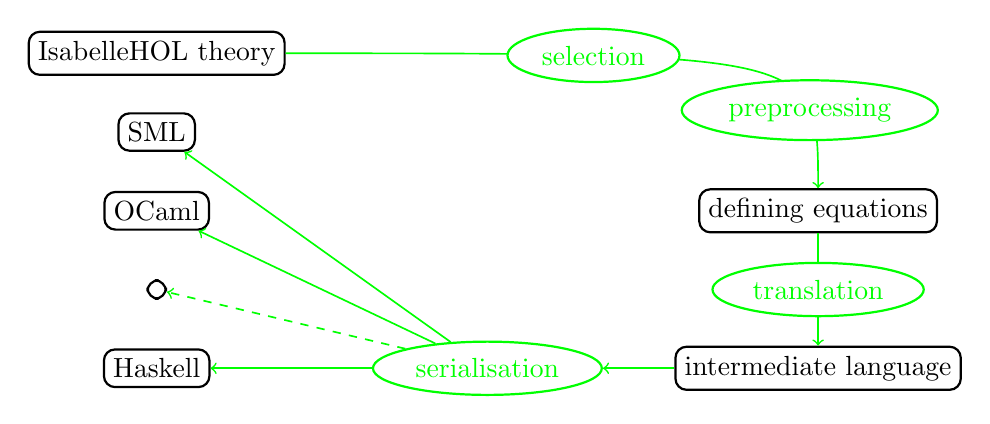
\begin{tikzpicture}[x = 4.2cm, y = 1cm]
      \tikzstyle entity=[rounded corners, draw, thick, color = black, fill = white];
      \tikzstyle process=[ellipse, draw, thick, color = green, fill = white];
      \tikzstyle process_arrow=[->, semithick, color = green];
      \node (HOL) at (0, 4) [style=entity] {\isa{Isabelle{\isacharslash}HOL} theory};
      \node (eqn) at (2, 2) [style=entity] {defining equations};
      \node (iml) at (2, 0) [style=entity] {intermediate language};
      \node (seri) at (1, 0) [style=process] {serialisation};
      \node (SML) at (0, 3) [style=entity] {\isa{SML}};
      \node (OCaml) at (0, 2) [style=entity] {\isa{OCaml}};
      \node (further) at (0, 1) [style=entity] {\isa{{\isasymdots}}};
      \node (Haskell) at (0, 0) [style=entity] {\isa{Haskell}};
      \draw [style=process_arrow] (HOL) .. controls (2, 4) ..
        node [style=process, near start] {selection}
        node [style=process, near end] {preprocessing}
        (eqn);
      \draw [style=process_arrow] (eqn) -- node (transl) [style=process] {translation} (iml);
      \draw [style=process_arrow] (iml) -- (seri);
      \draw [style=process_arrow] (seri) -- (SML);
      \draw [style=process_arrow] (seri) -- (OCaml);
      \draw [style=process_arrow, dashed] (seri) -- (further);
      \draw [style=process_arrow] (seri) -- (Haskell);
    \end{tikzpicture}
    \caption{Code generator architecture}
    \label{fig:arch}
  \end{figure}

  The code generator employs a notion of executability
  for three foundational executable ingredients known
  from functional programming:
  \emph{defining equations}, \emph{datatypes}, and
  \emph{type classes}.  A defining equation as a first approximation
  is a theorem of the form \isa{f\ t\isactrlisub {\isadigit{1}}\ t\isactrlisub {\isadigit{2}}\ {\isasymdots}\ t\isactrlisub n\ {\isasymequiv}\ t}
  (an equation headed by a constant \isa{f} with arguments
  \isa{t\isactrlisub {\isadigit{1}}\ t\isactrlisub {\isadigit{2}}\ {\isasymdots}\ t\isactrlisub n} and right hand side \isa{t}).
  Code generation aims to turn defining equations
  into a functional program.  This is achieved by three major
  components which operate sequentially, i.e. the result of one is
  the input
  of the next in the chain,  see diagram \ref{fig:arch}:

  \begin{itemize}

    \item Out of the vast collection of theorems proven in a
      \qn{theory}, a reasonable subset modelling
      defining equations is \qn{selected}.

    \item On those selected theorems, certain
      transformations are carried out
      (\qn{preprocessing}).  Their purpose is to turn theorems
      representing non- or badly executable
      specifications into equivalent but executable counterparts.
      The result is a structured collection of \qn{code theorems}.

    \item Before the selected defining equations are continued with,
      they can be \qn{preprocessed}, i.e. subjected to theorem
      transformations.  This \qn{preprocessor} is an interface which
      allows to apply
      the full expressiveness of ML-based theorem transformations
      to code generation;  motivating examples are shown below, see
      \secref{sec:preproc}.
      The result of the preprocessing step is a structured collection
      of defining equations.

    \item These defining equations are \qn{translated} to a program
      in an abstract intermediate language.  Think of it as a kind
      of \qt{Mini-Haskell} with four \qn{statements}: \isa{data}
      (for datatypes), \isa{fun} (stemming from defining equations),
      also \isa{class} and \isa{inst} (for type classes).

    \item Finally, the abstract program is \qn{serialised} into concrete
      source code of a target language.

  \end{itemize}

  \noindent From these steps, only the two last are carried out outside the logic;  by
  keeping this layer as thin as possible, the amount of code to trust is
  kept to a minimum.%
\end{isamarkuptext}%
\isamarkuptrue%
%
\isadelimtheory
%
\endisadelimtheory
%
\isatagtheory
\isacommand{end}\isamarkupfalse%
%
\endisatagtheory
{\isafoldtheory}%
%
\isadelimtheory
%
\endisadelimtheory
\isanewline
\end{isabellebody}%
%%% Local Variables:
%%% mode: latex
%%% TeX-master: "root"
%%% End:

%
\begin{isabellebody}%
\def\isabellecontext{Program}%
%
\isadelimtheory
%
\endisadelimtheory
%
\isatagtheory
\isacommand{theory}\isamarkupfalse%
\ Program\isanewline
\isakeyword{imports}\ Introduction\isanewline
\isakeyword{begin}%
\endisatagtheory
{\isafoldtheory}%
%
\isadelimtheory
%
\endisadelimtheory
%
\isamarkupsection{Turning Theories into Programs \label{sec:program}%
}
\isamarkuptrue%
%
\isamarkupsubsection{The \isa{Isabelle{\isacharslash}HOL} default setup%
}
\isamarkuptrue%
%
\begin{isamarkuptext}%
We have already seen how by default equations stemming from
  \hyperlink{command.definition}{\mbox{\isa{\isacommand{definition}}}}/\hyperlink{command.primrec}{\mbox{\isa{\isacommand{primrec}}}}/\hyperlink{command.fun}{\mbox{\isa{\isacommand{fun}}}}
  statements are used for code generation.  This default behaviour
  can be changed, e.g. by providing different code equations.
  All kinds of customisation shown in this section is \emph{safe}
  in the sense that the user does not have to worry about
  correctness -- all programs generatable that way are partially
  correct.%
\end{isamarkuptext}%
\isamarkuptrue%
%
\isamarkupsubsection{Selecting code equations%
}
\isamarkuptrue%
%
\begin{isamarkuptext}%
Coming back to our introductory example, we
  could provide an alternative code equations for \isa{dequeue}
  explicitly:%
\end{isamarkuptext}%
\isamarkuptrue%
%
\isadelimquote
%
\endisadelimquote
%
\isatagquote
\isacommand{lemma}\isamarkupfalse%
\ {\isacharbrackleft}code{\isacharbrackright}{\isacharcolon}\isanewline
\ \ {\isachardoublequoteopen}dequeue\ {\isacharparenleft}AQueue\ xs\ {\isacharbrackleft}{\isacharbrackright}{\isacharparenright}\ {\isacharequal}\isanewline
\ \ \ \ \ {\isacharparenleft}if\ xs\ {\isacharequal}\ {\isacharbrackleft}{\isacharbrackright}\ then\ {\isacharparenleft}None{\isacharcomma}\ AQueue\ {\isacharbrackleft}{\isacharbrackright}\ {\isacharbrackleft}{\isacharbrackright}{\isacharparenright}\isanewline
\ \ \ \ \ \ \ else\ dequeue\ {\isacharparenleft}AQueue\ {\isacharbrackleft}{\isacharbrackright}\ {\isacharparenleft}rev\ xs{\isacharparenright}{\isacharparenright}{\isacharparenright}{\isachardoublequoteclose}\isanewline
\ \ {\isachardoublequoteopen}dequeue\ {\isacharparenleft}AQueue\ xs\ {\isacharparenleft}y\ {\isacharhash}\ ys{\isacharparenright}{\isacharparenright}\ {\isacharequal}\isanewline
\ \ \ \ \ {\isacharparenleft}Some\ y{\isacharcomma}\ AQueue\ xs\ ys{\isacharparenright}{\isachardoublequoteclose}\isanewline
\ \ \isacommand{by}\isamarkupfalse%
\ {\isacharparenleft}cases\ xs{\isacharcomma}\ simp{\isacharunderscore}all{\isacharparenright}\ {\isacharparenleft}cases\ {\isachardoublequoteopen}rev\ xs{\isachardoublequoteclose}{\isacharcomma}\ simp{\isacharunderscore}all{\isacharparenright}%
\endisatagquote
{\isafoldquote}%
%
\isadelimquote
%
\endisadelimquote
%
\begin{isamarkuptext}%
\noindent The annotation \isa{{\isacharbrackleft}code{\isacharbrackright}} is an \isa{Isar}
  \isa{attribute} which states that the given theorems should be
  considered as code equations for a \isa{fun} statement --
  the corresponding constant is determined syntactically.  The resulting code:%
\end{isamarkuptext}%
\isamarkuptrue%
%
\isadelimquote
%
\endisadelimquote
%
\isatagquote
%
\begin{isamarkuptext}%
\isatypewriter%
\noindent%
\hspace*{0pt}dequeue ::~forall a.~Queue a -> (Maybe a,~Queue a);\\
\hspace*{0pt}dequeue (AQueue xs (y :~ys)) = (Just y,~AQueue xs ys);\\
\hspace*{0pt}dequeue (AQueue xs []) =\\
\hspace*{0pt} ~(if nulla xs then (Nothing,~AQueue [] [])\\
\hspace*{0pt} ~~~else dequeue (AQueue [] (rev xs)));%
\end{isamarkuptext}%
\isamarkuptrue%
%
\endisatagquote
{\isafoldquote}%
%
\isadelimquote
%
\endisadelimquote
%
\begin{isamarkuptext}%
\noindent You may note that the equality test \isa{xs\ {\isacharequal}\ {\isacharbrackleft}{\isacharbrackright}} has been
  replaced by the predicate \isa{null\ xs}.  This is due to the default
  setup in the \qn{preprocessor} to be discussed further below (\secref{sec:preproc}).

  Changing the default constructor set of datatypes is also
  possible.  See \secref{sec:datatypes} for an example.

  As told in \secref{sec:concept}, code generation is based
  on a structured collection of code theorems.
  For explorative purpose, this collection
  may be inspected using the \hyperlink{command.code-thms}{\mbox{\isa{\isacommand{code{\isacharunderscore}thms}}}} command:%
\end{isamarkuptext}%
\isamarkuptrue%
%
\isadelimquote
%
\endisadelimquote
%
\isatagquote
\isacommand{code{\isacharunderscore}thms}\isamarkupfalse%
\ dequeue%
\endisatagquote
{\isafoldquote}%
%
\isadelimquote
%
\endisadelimquote
%
\begin{isamarkuptext}%
\noindent prints a table with \emph{all} code equations
  for \isa{dequeue}, including
  \emph{all} code equations those equations depend
  on recursively.
  
  Similarly, the \hyperlink{command.code-deps}{\mbox{\isa{\isacommand{code{\isacharunderscore}deps}}}} command shows a graph
  visualising dependencies between code equations.%
\end{isamarkuptext}%
\isamarkuptrue%
%
\isamarkupsubsection{\isa{class} and \isa{instantiation}%
}
\isamarkuptrue%
%
\begin{isamarkuptext}%
Concerning type classes and code generation, let us examine an example
  from abstract algebra:%
\end{isamarkuptext}%
\isamarkuptrue%
%
\isadelimquote
%
\endisadelimquote
%
\isatagquote
\isacommand{class}\isamarkupfalse%
\ semigroup\ {\isacharequal}\isanewline
\ \ \isakeyword{fixes}\ mult\ {\isacharcolon}{\isacharcolon}\ {\isachardoublequoteopen}{\isacharprime}a\ {\isasymRightarrow}\ {\isacharprime}a\ {\isasymRightarrow}\ {\isacharprime}a{\isachardoublequoteclose}\ {\isacharparenleft}\isakeyword{infixl}\ {\isachardoublequoteopen}{\isasymotimes}{\isachardoublequoteclose}\ {\isadigit{7}}{\isadigit{0}}{\isacharparenright}\isanewline
\ \ \isakeyword{assumes}\ assoc{\isacharcolon}\ {\isachardoublequoteopen}{\isacharparenleft}x\ {\isasymotimes}\ y{\isacharparenright}\ {\isasymotimes}\ z\ {\isacharequal}\ x\ {\isasymotimes}\ {\isacharparenleft}y\ {\isasymotimes}\ z{\isacharparenright}{\isachardoublequoteclose}\isanewline
\isanewline
\isacommand{class}\isamarkupfalse%
\ monoid\ {\isacharequal}\ semigroup\ {\isacharplus}\isanewline
\ \ \isakeyword{fixes}\ neutral\ {\isacharcolon}{\isacharcolon}\ {\isacharprime}a\ {\isacharparenleft}{\isachardoublequoteopen}{\isasymone}{\isachardoublequoteclose}{\isacharparenright}\isanewline
\ \ \isakeyword{assumes}\ neutl{\isacharcolon}\ {\isachardoublequoteopen}{\isasymone}\ {\isasymotimes}\ x\ {\isacharequal}\ x{\isachardoublequoteclose}\isanewline
\ \ \ \ \isakeyword{and}\ neutr{\isacharcolon}\ {\isachardoublequoteopen}x\ {\isasymotimes}\ {\isasymone}\ {\isacharequal}\ x{\isachardoublequoteclose}\isanewline
\isanewline
\isacommand{instantiation}\isamarkupfalse%
\ nat\ {\isacharcolon}{\isacharcolon}\ monoid\isanewline
\isakeyword{begin}\isanewline
\isanewline
\isacommand{primrec}\isamarkupfalse%
\ mult{\isacharunderscore}nat\ \isakeyword{where}\isanewline
\ \ \ \ {\isachardoublequoteopen}{\isadigit{0}}\ {\isasymotimes}\ n\ {\isacharequal}\ {\isacharparenleft}{\isadigit{0}}{\isasymColon}nat{\isacharparenright}{\isachardoublequoteclose}\isanewline
\ \ {\isacharbar}\ {\isachardoublequoteopen}Suc\ m\ {\isasymotimes}\ n\ {\isacharequal}\ n\ {\isacharplus}\ m\ {\isasymotimes}\ n{\isachardoublequoteclose}\isanewline
\isanewline
\isacommand{definition}\isamarkupfalse%
\ neutral{\isacharunderscore}nat\ \isakeyword{where}\isanewline
\ \ {\isachardoublequoteopen}{\isasymone}\ {\isacharequal}\ Suc\ {\isadigit{0}}{\isachardoublequoteclose}\isanewline
\isanewline
\isacommand{lemma}\isamarkupfalse%
\ add{\isacharunderscore}mult{\isacharunderscore}distrib{\isacharcolon}\isanewline
\ \ \isakeyword{fixes}\ n\ m\ q\ {\isacharcolon}{\isacharcolon}\ nat\isanewline
\ \ \isakeyword{shows}\ {\isachardoublequoteopen}{\isacharparenleft}n\ {\isacharplus}\ m{\isacharparenright}\ {\isasymotimes}\ q\ {\isacharequal}\ n\ {\isasymotimes}\ q\ {\isacharplus}\ m\ {\isasymotimes}\ q{\isachardoublequoteclose}\isanewline
\ \ \isacommand{by}\isamarkupfalse%
\ {\isacharparenleft}induct\ n{\isacharparenright}\ simp{\isacharunderscore}all\isanewline
\isanewline
\isacommand{instance}\isamarkupfalse%
\ \isacommand{proof}\isamarkupfalse%
\isanewline
\ \ \isacommand{fix}\isamarkupfalse%
\ m\ n\ q\ {\isacharcolon}{\isacharcolon}\ nat\isanewline
\ \ \isacommand{show}\isamarkupfalse%
\ {\isachardoublequoteopen}m\ {\isasymotimes}\ n\ {\isasymotimes}\ q\ {\isacharequal}\ m\ {\isasymotimes}\ {\isacharparenleft}n\ {\isasymotimes}\ q{\isacharparenright}{\isachardoublequoteclose}\isanewline
\ \ \ \ \isacommand{by}\isamarkupfalse%
\ {\isacharparenleft}induct\ m{\isacharparenright}\ {\isacharparenleft}simp{\isacharunderscore}all\ add{\isacharcolon}\ add{\isacharunderscore}mult{\isacharunderscore}distrib{\isacharparenright}\isanewline
\ \ \isacommand{show}\isamarkupfalse%
\ {\isachardoublequoteopen}{\isasymone}\ {\isasymotimes}\ n\ {\isacharequal}\ n{\isachardoublequoteclose}\isanewline
\ \ \ \ \isacommand{by}\isamarkupfalse%
\ {\isacharparenleft}simp\ add{\isacharcolon}\ neutral{\isacharunderscore}nat{\isacharunderscore}def{\isacharparenright}\isanewline
\ \ \isacommand{show}\isamarkupfalse%
\ {\isachardoublequoteopen}m\ {\isasymotimes}\ {\isasymone}\ {\isacharequal}\ m{\isachardoublequoteclose}\isanewline
\ \ \ \ \isacommand{by}\isamarkupfalse%
\ {\isacharparenleft}induct\ m{\isacharparenright}\ {\isacharparenleft}simp{\isacharunderscore}all\ add{\isacharcolon}\ neutral{\isacharunderscore}nat{\isacharunderscore}def{\isacharparenright}\isanewline
\isacommand{qed}\isamarkupfalse%
\isanewline
\isanewline
\isacommand{end}\isamarkupfalse%
%
\endisatagquote
{\isafoldquote}%
%
\isadelimquote
%
\endisadelimquote
%
\begin{isamarkuptext}%
\noindent We define the natural operation of the natural numbers
  on monoids:%
\end{isamarkuptext}%
\isamarkuptrue%
%
\isadelimquote
%
\endisadelimquote
%
\isatagquote
\isacommand{primrec}\isamarkupfalse%
\ {\isacharparenleft}\isakeyword{in}\ monoid{\isacharparenright}\ pow\ {\isacharcolon}{\isacharcolon}\ {\isachardoublequoteopen}nat\ {\isasymRightarrow}\ {\isacharprime}a\ {\isasymRightarrow}\ {\isacharprime}a{\isachardoublequoteclose}\ \isakeyword{where}\isanewline
\ \ \ \ {\isachardoublequoteopen}pow\ {\isadigit{0}}\ a\ {\isacharequal}\ {\isasymone}{\isachardoublequoteclose}\isanewline
\ \ {\isacharbar}\ {\isachardoublequoteopen}pow\ {\isacharparenleft}Suc\ n{\isacharparenright}\ a\ {\isacharequal}\ a\ {\isasymotimes}\ pow\ n\ a{\isachardoublequoteclose}%
\endisatagquote
{\isafoldquote}%
%
\isadelimquote
%
\endisadelimquote
%
\begin{isamarkuptext}%
\noindent This we use to define the discrete exponentiation function:%
\end{isamarkuptext}%
\isamarkuptrue%
%
\isadelimquote
%
\endisadelimquote
%
\isatagquote
\isacommand{definition}\isamarkupfalse%
\ bexp\ {\isacharcolon}{\isacharcolon}\ {\isachardoublequoteopen}nat\ {\isasymRightarrow}\ nat{\isachardoublequoteclose}\ \isakeyword{where}\isanewline
\ \ {\isachardoublequoteopen}bexp\ n\ {\isacharequal}\ pow\ n\ {\isacharparenleft}Suc\ {\isacharparenleft}Suc\ {\isadigit{0}}{\isacharparenright}{\isacharparenright}{\isachardoublequoteclose}%
\endisatagquote
{\isafoldquote}%
%
\isadelimquote
%
\endisadelimquote
%
\begin{isamarkuptext}%
\noindent The corresponding code:%
\end{isamarkuptext}%
\isamarkuptrue%
%
\isadelimquote
%
\endisadelimquote
%
\isatagquote
%
\begin{isamarkuptext}%
\isatypewriter%
\noindent%
\hspace*{0pt}module Example where {\char123}\\
\hspace*{0pt}\\
\hspace*{0pt}\\
\hspace*{0pt}data Nat = Zero{\char95}nat | Suc Nat;\\
\hspace*{0pt}\\
\hspace*{0pt}class Semigroup a where {\char123}\\
\hspace*{0pt} ~mult ::~a -> a -> a;\\
\hspace*{0pt}{\char125};\\
\hspace*{0pt}\\
\hspace*{0pt}class (Semigroup a) => Monoid a where {\char123}\\
\hspace*{0pt} ~neutral ::~a;\\
\hspace*{0pt}{\char125};\\
\hspace*{0pt}\\
\hspace*{0pt}pow ::~forall a.~(Monoid a) => Nat -> a -> a;\\
\hspace*{0pt}pow Zero{\char95}nat a = neutral;\\
\hspace*{0pt}pow (Suc n) a = mult a (pow n a);\\
\hspace*{0pt}\\
\hspace*{0pt}plus{\char95}nat ::~Nat -> Nat -> Nat;\\
\hspace*{0pt}plus{\char95}nat (Suc m) n = plus{\char95}nat m (Suc n);\\
\hspace*{0pt}plus{\char95}nat Zero{\char95}nat n = n;\\
\hspace*{0pt}\\
\hspace*{0pt}neutral{\char95}nat ::~Nat;\\
\hspace*{0pt}neutral{\char95}nat = Suc Zero{\char95}nat;\\
\hspace*{0pt}\\
\hspace*{0pt}mult{\char95}nat ::~Nat -> Nat -> Nat;\\
\hspace*{0pt}mult{\char95}nat Zero{\char95}nat n = Zero{\char95}nat;\\
\hspace*{0pt}mult{\char95}nat (Suc m) n = plus{\char95}nat n (mult{\char95}nat m n);\\
\hspace*{0pt}\\
\hspace*{0pt}instance Semigroup Nat where {\char123}\\
\hspace*{0pt} ~mult = mult{\char95}nat;\\
\hspace*{0pt}{\char125};\\
\hspace*{0pt}\\
\hspace*{0pt}instance Monoid Nat where {\char123}\\
\hspace*{0pt} ~neutral = neutral{\char95}nat;\\
\hspace*{0pt}{\char125};\\
\hspace*{0pt}\\
\hspace*{0pt}bexp ::~Nat -> Nat;\\
\hspace*{0pt}bexp n = pow n (Suc (Suc Zero{\char95}nat));\\
\hspace*{0pt}\\
\hspace*{0pt}{\char125}%
\end{isamarkuptext}%
\isamarkuptrue%
%
\endisatagquote
{\isafoldquote}%
%
\isadelimquote
%
\endisadelimquote
%
\begin{isamarkuptext}%
\noindent This is a convenient place to show how explicit dictionary construction
  manifests in generated code (here, the same example in \isa{SML}):%
\end{isamarkuptext}%
\isamarkuptrue%
%
\isadelimquote
%
\endisadelimquote
%
\isatagquote
%
\begin{isamarkuptext}%
\isatypewriter%
\noindent%
\hspace*{0pt}structure Example = \\
\hspace*{0pt}struct\\
\hspace*{0pt}\\
\hspace*{0pt}datatype nat = Zero{\char95}nat | Suc of nat;\\
\hspace*{0pt}\\
\hspace*{0pt}type 'a semigroup = {\char123}mult :~'a -> 'a -> 'a{\char125};\\
\hspace*{0pt}fun mult (A{\char95}:'a semigroup) = {\char35}mult A{\char95};\\
\hspace*{0pt}\\
\hspace*{0pt}type 'a monoid = {\char123}semigroup{\char95}monoid :~'a semigroup,~neutral :~'a{\char125};\\
\hspace*{0pt}fun semigroup{\char95}monoid (A{\char95}:'a monoid) = {\char35}semigroup{\char95}monoid A{\char95};\\
\hspace*{0pt}fun neutral (A{\char95}:'a monoid) = {\char35}neutral A{\char95};\\
\hspace*{0pt}\\
\hspace*{0pt}fun pow A{\char95}~Zero{\char95}nat a = neutral A{\char95}\\
\hspace*{0pt} ~| pow A{\char95}~(Suc n) a = mult (semigroup{\char95}monoid A{\char95}) a (pow A{\char95}~n a);\\
\hspace*{0pt}\\
\hspace*{0pt}fun plus{\char95}nat (Suc m) n = plus{\char95}nat m (Suc n)\\
\hspace*{0pt} ~| plus{\char95}nat Zero{\char95}nat n = n;\\
\hspace*{0pt}\\
\hspace*{0pt}val neutral{\char95}nat :~nat = Suc Zero{\char95}nat\\
\hspace*{0pt}\\
\hspace*{0pt}fun mult{\char95}nat Zero{\char95}nat n = Zero{\char95}nat\\
\hspace*{0pt} ~| mult{\char95}nat (Suc m) n = plus{\char95}nat n (mult{\char95}nat m n);\\
\hspace*{0pt}\\
\hspace*{0pt}val semigroup{\char95}nat = {\char123}mult = mult{\char95}nat{\char125}~:~nat semigroup;\\
\hspace*{0pt}\\
\hspace*{0pt}val monoid{\char95}nat = {\char123}semigroup{\char95}monoid = semigroup{\char95}nat,~neutral = neutral{\char95}nat{\char125}\\
\hspace*{0pt} ~:~nat monoid;\\
\hspace*{0pt}\\
\hspace*{0pt}fun bexp n = pow monoid{\char95}nat n (Suc (Suc Zero{\char95}nat));\\
\hspace*{0pt}\\
\hspace*{0pt}end;~(*struct Example*)%
\end{isamarkuptext}%
\isamarkuptrue%
%
\endisatagquote
{\isafoldquote}%
%
\isadelimquote
%
\endisadelimquote
%
\begin{isamarkuptext}%
\noindent Note the parameters with trailing underscore (\verb|A_|)
    which are the dictionary parameters.%
\end{isamarkuptext}%
\isamarkuptrue%
%
\isamarkupsubsection{The preprocessor \label{sec:preproc}%
}
\isamarkuptrue%
%
\begin{isamarkuptext}%
Before selected function theorems are turned into abstract
  code, a chain of definitional transformation steps is carried
  out: \emph{preprocessing}.  In essence, the preprocessor
  consists of two components: a \emph{simpset} and \emph{function transformers}.

  The \emph{simpset} allows to employ the full generality of the Isabelle
  simplifier.  Due to the interpretation of theorems
  as code equations, rewrites are applied to the right
  hand side and the arguments of the left hand side of an
  equation, but never to the constant heading the left hand side.
  An important special case are \emph{inline theorems} which may be
  declared and undeclared using the
  \emph{code inline} or \emph{code inline del} attribute respectively.

  Some common applications:%
\end{isamarkuptext}%
\isamarkuptrue%
%
\begin{itemize}
%
\begin{isamarkuptext}%
\item replacing non-executable constructs by executable ones:%
\end{isamarkuptext}%
\isamarkuptrue%
%
\isadelimquote
%
\endisadelimquote
%
\isatagquote
\isacommand{lemma}\isamarkupfalse%
\ {\isacharbrackleft}code\ inline{\isacharbrackright}{\isacharcolon}\isanewline
\ \ {\isachardoublequoteopen}x\ {\isasymin}\ set\ xs\ {\isasymlongleftrightarrow}\ x\ mem\ xs{\isachardoublequoteclose}\ \isacommand{by}\isamarkupfalse%
\ {\isacharparenleft}induct\ xs{\isacharparenright}\ simp{\isacharunderscore}all%
\endisatagquote
{\isafoldquote}%
%
\isadelimquote
%
\endisadelimquote
%
\begin{isamarkuptext}%
\item eliminating superfluous constants:%
\end{isamarkuptext}%
\isamarkuptrue%
%
\isadelimquote
%
\endisadelimquote
%
\isatagquote
\isacommand{lemma}\isamarkupfalse%
\ {\isacharbrackleft}code\ inline{\isacharbrackright}{\isacharcolon}\isanewline
\ \ {\isachardoublequoteopen}{\isadigit{1}}\ {\isacharequal}\ Suc\ {\isadigit{0}}{\isachardoublequoteclose}\ \isacommand{by}\isamarkupfalse%
\ simp%
\endisatagquote
{\isafoldquote}%
%
\isadelimquote
%
\endisadelimquote
%
\begin{isamarkuptext}%
\item replacing executable but inconvenient constructs:%
\end{isamarkuptext}%
\isamarkuptrue%
%
\isadelimquote
%
\endisadelimquote
%
\isatagquote
\isacommand{lemma}\isamarkupfalse%
\ {\isacharbrackleft}code\ inline{\isacharbrackright}{\isacharcolon}\isanewline
\ \ {\isachardoublequoteopen}xs\ {\isacharequal}\ {\isacharbrackleft}{\isacharbrackright}\ {\isasymlongleftrightarrow}\ List{\isachardot}null\ xs{\isachardoublequoteclose}\ \isacommand{by}\isamarkupfalse%
\ {\isacharparenleft}induct\ xs{\isacharparenright}\ simp{\isacharunderscore}all%
\endisatagquote
{\isafoldquote}%
%
\isadelimquote
%
\endisadelimquote
%
\end{itemize}
%
\begin{isamarkuptext}%
\noindent \emph{Function transformers} provide a very general interface,
  transforming a list of function theorems to another
  list of function theorems, provided that neither the heading
  constant nor its type change.  The \isa{{\isadigit{0}}} / \isa{Suc}
  pattern elimination implemented in
  theory \isa{Efficient{\isacharunderscore}Nat} (see \secref{eff_nat}) uses this
  interface.

  \noindent The current setup of the preprocessor may be inspected using
  the \hyperlink{command.print-codeproc}{\mbox{\isa{\isacommand{print{\isacharunderscore}codeproc}}}} command.
  \hyperlink{command.code-thms}{\mbox{\isa{\isacommand{code{\isacharunderscore}thms}}}} provides a convenient
  mechanism to inspect the impact of a preprocessor setup
  on code equations.

  \begin{warn}
    The attribute \emph{code unfold}
    associated with the \isa{SML\ code\ generator} also applies to
    the \isa{generic\ code\ generator}:
    \emph{code unfold} implies \emph{code inline}.
  \end{warn}%
\end{isamarkuptext}%
\isamarkuptrue%
%
\isamarkupsubsection{Datatypes \label{sec:datatypes}%
}
\isamarkuptrue%
%
\begin{isamarkuptext}%
Conceptually, any datatype is spanned by a set of
  \emph{constructors} of type \isa{{\isasymtau}\ {\isacharequal}\ {\isasymdots}\ {\isasymRightarrow}\ {\isasymkappa}\ {\isasymalpha}\isactrlisub {\isadigit{1}}\ {\isasymdots}\ {\isasymalpha}\isactrlisub n} where \isa{{\isacharbraceleft}{\isasymalpha}\isactrlisub {\isadigit{1}}{\isacharcomma}\ {\isasymdots}{\isacharcomma}\ {\isasymalpha}\isactrlisub n{\isacharbraceright}} is exactly the set of \emph{all} type variables in
  \isa{{\isasymtau}}.  The HOL datatype package by default registers any new
  datatype in the table of datatypes, which may be inspected using the
  \hyperlink{command.print-codesetup}{\mbox{\isa{\isacommand{print{\isacharunderscore}codesetup}}}} command.

  In some cases, it is appropriate to alter or extend this table.  As
  an example, we will develop an alternative representation of the
  queue example given in \secref{sec:intro}.  The amortised
  representation is convenient for generating code but exposes its
  \qt{implementation} details, which may be cumbersome when proving
  theorems about it.  Therefore, here a simple, straightforward
  representation of queues:%
\end{isamarkuptext}%
\isamarkuptrue%
%
\isadelimquote
%
\endisadelimquote
%
\isatagquote
\isacommand{datatype}\isamarkupfalse%
\ {\isacharprime}a\ queue\ {\isacharequal}\ Queue\ {\isachardoublequoteopen}{\isacharprime}a\ list{\isachardoublequoteclose}\isanewline
\isanewline
\isacommand{definition}\isamarkupfalse%
\ empty\ {\isacharcolon}{\isacharcolon}\ {\isachardoublequoteopen}{\isacharprime}a\ queue{\isachardoublequoteclose}\ \isakeyword{where}\isanewline
\ \ {\isachardoublequoteopen}empty\ {\isacharequal}\ Queue\ {\isacharbrackleft}{\isacharbrackright}{\isachardoublequoteclose}\isanewline
\isanewline
\isacommand{primrec}\isamarkupfalse%
\ enqueue\ {\isacharcolon}{\isacharcolon}\ {\isachardoublequoteopen}{\isacharprime}a\ {\isasymRightarrow}\ {\isacharprime}a\ queue\ {\isasymRightarrow}\ {\isacharprime}a\ queue{\isachardoublequoteclose}\ \isakeyword{where}\isanewline
\ \ {\isachardoublequoteopen}enqueue\ x\ {\isacharparenleft}Queue\ xs{\isacharparenright}\ {\isacharequal}\ Queue\ {\isacharparenleft}xs\ {\isacharat}\ {\isacharbrackleft}x{\isacharbrackright}{\isacharparenright}{\isachardoublequoteclose}\isanewline
\isanewline
\isacommand{fun}\isamarkupfalse%
\ dequeue\ {\isacharcolon}{\isacharcolon}\ {\isachardoublequoteopen}{\isacharprime}a\ queue\ {\isasymRightarrow}\ {\isacharprime}a\ option\ {\isasymtimes}\ {\isacharprime}a\ queue{\isachardoublequoteclose}\ \isakeyword{where}\isanewline
\ \ \ \ {\isachardoublequoteopen}dequeue\ {\isacharparenleft}Queue\ {\isacharbrackleft}{\isacharbrackright}{\isacharparenright}\ {\isacharequal}\ {\isacharparenleft}None{\isacharcomma}\ Queue\ {\isacharbrackleft}{\isacharbrackright}{\isacharparenright}{\isachardoublequoteclose}\isanewline
\ \ {\isacharbar}\ {\isachardoublequoteopen}dequeue\ {\isacharparenleft}Queue\ {\isacharparenleft}x\ {\isacharhash}\ xs{\isacharparenright}{\isacharparenright}\ {\isacharequal}\ {\isacharparenleft}Some\ x{\isacharcomma}\ Queue\ xs{\isacharparenright}{\isachardoublequoteclose}%
\endisatagquote
{\isafoldquote}%
%
\isadelimquote
%
\endisadelimquote
%
\begin{isamarkuptext}%
\noindent This we can use directly for proving;  for executing,
  we provide an alternative characterisation:%
\end{isamarkuptext}%
\isamarkuptrue%
%
\isadelimquote
%
\endisadelimquote
%
\isatagquote
\isacommand{definition}\isamarkupfalse%
\ AQueue\ {\isacharcolon}{\isacharcolon}\ {\isachardoublequoteopen}{\isacharprime}a\ list\ {\isasymRightarrow}\ {\isacharprime}a\ list\ {\isasymRightarrow}\ {\isacharprime}a\ queue{\isachardoublequoteclose}\ \isakeyword{where}\isanewline
\ \ {\isachardoublequoteopen}AQueue\ xs\ ys\ {\isacharequal}\ Queue\ {\isacharparenleft}ys\ {\isacharat}\ rev\ xs{\isacharparenright}{\isachardoublequoteclose}\isanewline
\isanewline
\isacommand{code{\isacharunderscore}datatype}\isamarkupfalse%
\ AQueue%
\endisatagquote
{\isafoldquote}%
%
\isadelimquote
%
\endisadelimquote
%
\begin{isamarkuptext}%
\noindent Here we define a \qt{constructor} \isa{AQueue} which
  is defined in terms of \isa{Queue} and interprets its arguments
  according to what the \emph{content} of an amortised queue is supposed
  to be.  Equipped with this, we are able to prove the following equations
  for our primitive queue operations which \qt{implement} the simple
  queues in an amortised fashion:%
\end{isamarkuptext}%
\isamarkuptrue%
%
\isadelimquote
%
\endisadelimquote
%
\isatagquote
\isacommand{lemma}\isamarkupfalse%
\ empty{\isacharunderscore}AQueue\ {\isacharbrackleft}code{\isacharbrackright}{\isacharcolon}\isanewline
\ \ {\isachardoublequoteopen}empty\ {\isacharequal}\ AQueue\ {\isacharbrackleft}{\isacharbrackright}\ {\isacharbrackleft}{\isacharbrackright}{\isachardoublequoteclose}\isanewline
\ \ \isacommand{unfolding}\isamarkupfalse%
\ AQueue{\isacharunderscore}def\ empty{\isacharunderscore}def\ \isacommand{by}\isamarkupfalse%
\ simp\isanewline
\isanewline
\isacommand{lemma}\isamarkupfalse%
\ enqueue{\isacharunderscore}AQueue\ {\isacharbrackleft}code{\isacharbrackright}{\isacharcolon}\isanewline
\ \ {\isachardoublequoteopen}enqueue\ x\ {\isacharparenleft}AQueue\ xs\ ys{\isacharparenright}\ {\isacharequal}\ AQueue\ {\isacharparenleft}x\ {\isacharhash}\ xs{\isacharparenright}\ ys{\isachardoublequoteclose}\isanewline
\ \ \isacommand{unfolding}\isamarkupfalse%
\ AQueue{\isacharunderscore}def\ \isacommand{by}\isamarkupfalse%
\ simp\isanewline
\isanewline
\isacommand{lemma}\isamarkupfalse%
\ dequeue{\isacharunderscore}AQueue\ {\isacharbrackleft}code{\isacharbrackright}{\isacharcolon}\isanewline
\ \ {\isachardoublequoteopen}dequeue\ {\isacharparenleft}AQueue\ xs\ {\isacharbrackleft}{\isacharbrackright}{\isacharparenright}\ {\isacharequal}\isanewline
\ \ \ \ {\isacharparenleft}if\ xs\ {\isacharequal}\ {\isacharbrackleft}{\isacharbrackright}\ then\ {\isacharparenleft}None{\isacharcomma}\ AQueue\ {\isacharbrackleft}{\isacharbrackright}\ {\isacharbrackleft}{\isacharbrackright}{\isacharparenright}\isanewline
\ \ \ \ else\ dequeue\ {\isacharparenleft}AQueue\ {\isacharbrackleft}{\isacharbrackright}\ {\isacharparenleft}rev\ xs{\isacharparenright}{\isacharparenright}{\isacharparenright}{\isachardoublequoteclose}\isanewline
\ \ {\isachardoublequoteopen}dequeue\ {\isacharparenleft}AQueue\ xs\ {\isacharparenleft}y\ {\isacharhash}\ ys{\isacharparenright}{\isacharparenright}\ {\isacharequal}\ {\isacharparenleft}Some\ y{\isacharcomma}\ AQueue\ xs\ ys{\isacharparenright}{\isachardoublequoteclose}\isanewline
\ \ \isacommand{unfolding}\isamarkupfalse%
\ AQueue{\isacharunderscore}def\ \isacommand{by}\isamarkupfalse%
\ simp{\isacharunderscore}all%
\endisatagquote
{\isafoldquote}%
%
\isadelimquote
%
\endisadelimquote
%
\begin{isamarkuptext}%
\noindent For completeness, we provide a substitute for the
  \isa{case} combinator on queues:%
\end{isamarkuptext}%
\isamarkuptrue%
%
\isadelimquote
%
\endisadelimquote
%
\isatagquote
\isacommand{lemma}\isamarkupfalse%
\ queue{\isacharunderscore}case{\isacharunderscore}AQueue\ {\isacharbrackleft}code{\isacharbrackright}{\isacharcolon}\isanewline
\ \ {\isachardoublequoteopen}queue{\isacharunderscore}case\ f\ {\isacharparenleft}AQueue\ xs\ ys{\isacharparenright}\ {\isacharequal}\ f\ {\isacharparenleft}ys\ {\isacharat}\ rev\ xs{\isacharparenright}{\isachardoublequoteclose}\isanewline
\ \ \isacommand{unfolding}\isamarkupfalse%
\ AQueue{\isacharunderscore}def\ \isacommand{by}\isamarkupfalse%
\ simp%
\endisatagquote
{\isafoldquote}%
%
\isadelimquote
%
\endisadelimquote
%
\begin{isamarkuptext}%
\noindent The resulting code looks as expected:%
\end{isamarkuptext}%
\isamarkuptrue%
%
\isadelimquote
%
\endisadelimquote
%
\isatagquote
%
\begin{isamarkuptext}%
\isatypewriter%
\noindent%
\hspace*{0pt}structure Example = \\
\hspace*{0pt}struct\\
\hspace*{0pt}\\
\hspace*{0pt}fun foldl f a [] = a\\
\hspace*{0pt} ~| foldl f a (x ::~xs) = foldl f (f a x) xs;\\
\hspace*{0pt}\\
\hspace*{0pt}fun rev xs = foldl (fn xsa => fn x => x ::~xsa) [] xs;\\
\hspace*{0pt}\\
\hspace*{0pt}fun null [] = true\\
\hspace*{0pt} ~| null (x ::~xs) = false;\\
\hspace*{0pt}\\
\hspace*{0pt}datatype 'a queue = AQueue of 'a list * 'a list;\\
\hspace*{0pt}\\
\hspace*{0pt}val empty :~'a queue = AQueue ([],~[])\\
\hspace*{0pt}\\
\hspace*{0pt}fun dequeue (AQueue (xs,~y ::~ys)) = (SOME y,~AQueue (xs,~ys))\\
\hspace*{0pt} ~| dequeue (AQueue (xs,~[])) =\\
\hspace*{0pt} ~~~(if null xs then (NONE,~AQueue ([],~[]))\\
\hspace*{0pt} ~~~~~else dequeue (AQueue ([],~rev xs)));\\
\hspace*{0pt}\\
\hspace*{0pt}fun enqueue x (AQueue (xs,~ys)) = AQueue (x ::~xs,~ys);\\
\hspace*{0pt}\\
\hspace*{0pt}end;~(*struct Example*)%
\end{isamarkuptext}%
\isamarkuptrue%
%
\endisatagquote
{\isafoldquote}%
%
\isadelimquote
%
\endisadelimquote
%
\begin{isamarkuptext}%
\noindent From this example, it can be glimpsed that using own
  constructor sets is a little delicate since it changes the set of
  valid patterns for values of that type.  Without going into much
  detail, here some practical hints:

  \begin{itemize}

    \item When changing the constructor set for datatypes, take care
      to provide alternative equations for the \isa{case} combinator.

    \item Values in the target language need not to be normalised --
      different values in the target language may represent the same
      value in the logic.

    \item Usually, a good methodology to deal with the subtleties of
      pattern matching is to see the type as an abstract type: provide
      a set of operations which operate on the concrete representation
      of the type, and derive further operations by combinations of
      these primitive ones, without relying on a particular
      representation.

  \end{itemize}%
\end{isamarkuptext}%
\isamarkuptrue%
%
\isamarkupsubsection{Equality%
}
\isamarkuptrue%
%
\begin{isamarkuptext}%
Surely you have already noticed how equality is treated
  by the code generator:%
\end{isamarkuptext}%
\isamarkuptrue%
%
\isadelimquote
%
\endisadelimquote
%
\isatagquote
\isacommand{primrec}\isamarkupfalse%
\ collect{\isacharunderscore}duplicates\ {\isacharcolon}{\isacharcolon}\ {\isachardoublequoteopen}{\isacharprime}a\ list\ {\isasymRightarrow}\ {\isacharprime}a\ list\ {\isasymRightarrow}\ {\isacharprime}a\ list\ {\isasymRightarrow}\ {\isacharprime}a\ list{\isachardoublequoteclose}\ \isakeyword{where}\isanewline
\ \ {\isachardoublequoteopen}collect{\isacharunderscore}duplicates\ xs\ ys\ {\isacharbrackleft}{\isacharbrackright}\ {\isacharequal}\ xs{\isachardoublequoteclose}\isanewline
\ \ {\isacharbar}\ {\isachardoublequoteopen}collect{\isacharunderscore}duplicates\ xs\ ys\ {\isacharparenleft}z{\isacharhash}zs{\isacharparenright}\ {\isacharequal}\ {\isacharparenleft}if\ z\ {\isasymin}\ set\ xs\isanewline
\ \ \ \ \ \ then\ if\ z\ {\isasymin}\ set\ ys\isanewline
\ \ \ \ \ \ \ \ then\ collect{\isacharunderscore}duplicates\ xs\ ys\ zs\isanewline
\ \ \ \ \ \ \ \ else\ collect{\isacharunderscore}duplicates\ xs\ {\isacharparenleft}z{\isacharhash}ys{\isacharparenright}\ zs\isanewline
\ \ \ \ \ \ else\ collect{\isacharunderscore}duplicates\ {\isacharparenleft}z{\isacharhash}xs{\isacharparenright}\ {\isacharparenleft}z{\isacharhash}ys{\isacharparenright}\ zs{\isacharparenright}{\isachardoublequoteclose}%
\endisatagquote
{\isafoldquote}%
%
\isadelimquote
%
\endisadelimquote
%
\begin{isamarkuptext}%
\noindent The membership test during preprocessing is rewritten,
  resulting in \isa{op\ mem}, which itself
  performs an explicit equality check.%
\end{isamarkuptext}%
\isamarkuptrue%
%
\isadelimquote
%
\endisadelimquote
%
\isatagquote
%
\begin{isamarkuptext}%
\isatypewriter%
\noindent%
\hspace*{0pt}structure Example = \\
\hspace*{0pt}struct\\
\hspace*{0pt}\\
\hspace*{0pt}type 'a eq = {\char123}eq :~'a -> 'a -> bool{\char125};\\
\hspace*{0pt}fun eq (A{\char95}:'a eq) = {\char35}eq A{\char95};\\
\hspace*{0pt}\\
\hspace*{0pt}fun eqa A{\char95}~a b = eq A{\char95}~a b;\\
\hspace*{0pt}\\
\hspace*{0pt}fun member A{\char95}~x [] = false\\
\hspace*{0pt} ~| member A{\char95}~x (y ::~ys) = eqa A{\char95}~x y orelse member A{\char95}~x ys;\\
\hspace*{0pt}\\
\hspace*{0pt}fun collect{\char95}duplicates A{\char95}~xs ys [] = xs\\
\hspace*{0pt} ~| collect{\char95}duplicates A{\char95}~xs ys (z ::~zs) =\\
\hspace*{0pt} ~~~(if member A{\char95}~z xs\\
\hspace*{0pt} ~~~~~then (if member A{\char95}~z ys then collect{\char95}duplicates A{\char95}~xs ys zs\\
\hspace*{0pt} ~~~~~~~~~~~~else collect{\char95}duplicates A{\char95}~xs (z ::~ys) zs)\\
\hspace*{0pt} ~~~~~else collect{\char95}duplicates A{\char95}~(z ::~xs) (z ::~ys) zs);\\
\hspace*{0pt}\\
\hspace*{0pt}end;~(*struct Example*)%
\end{isamarkuptext}%
\isamarkuptrue%
%
\endisatagquote
{\isafoldquote}%
%
\isadelimquote
%
\endisadelimquote
%
\begin{isamarkuptext}%
\noindent Obviously, polymorphic equality is implemented the Haskell
  way using a type class.  How is this achieved?  HOL introduces
  an explicit class \isa{eq} with a corresponding operation
  \isa{eq{\isacharunderscore}class{\isachardot}eq} such that \isa{eq{\isacharunderscore}class{\isachardot}eq\ {\isacharequal}\ op\ {\isacharequal}}.
  The preprocessing framework does the rest by propagating the
  \isa{eq} constraints through all dependent code equations.
  For datatypes, instances of \isa{eq} are implicitly derived
  when possible.  For other types, you may instantiate \isa{eq}
  manually like any other type class.

  Though this \isa{eq} class is designed to get rarely in
  the way, in some cases the automatically derived code equations
  for equality on a particular type may not be appropriate.
  As example, watch the following datatype representing
  monomorphic parametric types (where type constructors
  are referred to by natural numbers):%
\end{isamarkuptext}%
\isamarkuptrue%
%
\isadelimquote
%
\endisadelimquote
%
\isatagquote
\isacommand{datatype}\isamarkupfalse%
\ monotype\ {\isacharequal}\ Mono\ nat\ {\isachardoublequoteopen}monotype\ list{\isachardoublequoteclose}%
\endisatagquote
{\isafoldquote}%
%
\isadelimquote
%
\endisadelimquote
%
\isadelimproof
%
\endisadelimproof
%
\isatagproof
%
\endisatagproof
{\isafoldproof}%
%
\isadelimproof
%
\endisadelimproof
%
\begin{isamarkuptext}%
\noindent Then code generation for SML would fail with a message
  that the generated code contains illegal mutual dependencies:
  the theorem \isa{eq{\isacharunderscore}class{\isachardot}eq\ {\isacharparenleft}Mono\ tyco{\isadigit{1}}\ typargs{\isadigit{1}}{\isacharparenright}\ {\isacharparenleft}Mono\ tyco{\isadigit{2}}\ typargs{\isadigit{2}}{\isacharparenright}\ {\isasymequiv}\ eq{\isacharunderscore}class{\isachardot}eq\ tyco{\isadigit{1}}\ tyco{\isadigit{2}}\ {\isasymand}\ eq{\isacharunderscore}class{\isachardot}eq\ typargs{\isadigit{1}}\ typargs{\isadigit{2}}} already requires the
  instance \isa{monotype\ {\isasymColon}\ eq}, which itself requires
  \isa{eq{\isacharunderscore}class{\isachardot}eq\ {\isacharparenleft}Mono\ tyco{\isadigit{1}}\ typargs{\isadigit{1}}{\isacharparenright}\ {\isacharparenleft}Mono\ tyco{\isadigit{2}}\ typargs{\isadigit{2}}{\isacharparenright}\ {\isasymequiv}\ eq{\isacharunderscore}class{\isachardot}eq\ tyco{\isadigit{1}}\ tyco{\isadigit{2}}\ {\isasymand}\ eq{\isacharunderscore}class{\isachardot}eq\ typargs{\isadigit{1}}\ typargs{\isadigit{2}}};  Haskell has no problem with mutually
  recursive \isa{instance} and \isa{function} definitions,
  but the SML serialiser does not support this.

  In such cases, you have to provide your own equality equations
  involving auxiliary constants.  In our case,
  \isa{list{\isacharunderscore}all{\isadigit{2}}} can do the job:%
\end{isamarkuptext}%
\isamarkuptrue%
%
\isadelimquote
%
\endisadelimquote
%
\isatagquote
\isacommand{lemma}\isamarkupfalse%
\ monotype{\isacharunderscore}eq{\isacharunderscore}list{\isacharunderscore}all{\isadigit{2}}\ {\isacharbrackleft}code{\isacharbrackright}{\isacharcolon}\isanewline
\ \ {\isachardoublequoteopen}eq{\isacharunderscore}class{\isachardot}eq\ {\isacharparenleft}Mono\ tyco{\isadigit{1}}\ typargs{\isadigit{1}}{\isacharparenright}\ {\isacharparenleft}Mono\ tyco{\isadigit{2}}\ typargs{\isadigit{2}}{\isacharparenright}\ {\isasymlongleftrightarrow}\isanewline
\ \ \ \ \ eq{\isacharunderscore}class{\isachardot}eq\ tyco{\isadigit{1}}\ tyco{\isadigit{2}}\ {\isasymand}\ list{\isacharunderscore}all{\isadigit{2}}\ eq{\isacharunderscore}class{\isachardot}eq\ typargs{\isadigit{1}}\ typargs{\isadigit{2}}{\isachardoublequoteclose}\isanewline
\ \ \isacommand{by}\isamarkupfalse%
\ {\isacharparenleft}simp\ add{\isacharcolon}\ eq\ list{\isacharunderscore}all{\isadigit{2}}{\isacharunderscore}eq\ {\isacharbrackleft}symmetric{\isacharbrackright}{\isacharparenright}%
\endisatagquote
{\isafoldquote}%
%
\isadelimquote
%
\endisadelimquote
%
\begin{isamarkuptext}%
\noindent does not depend on instance \isa{monotype\ {\isasymColon}\ eq}:%
\end{isamarkuptext}%
\isamarkuptrue%
%
\isadelimquote
%
\endisadelimquote
%
\isatagquote
%
\begin{isamarkuptext}%
\isatypewriter%
\noindent%
\hspace*{0pt}structure Example = \\
\hspace*{0pt}struct\\
\hspace*{0pt}\\
\hspace*{0pt}datatype nat = Zero{\char95}nat | Suc of nat;\\
\hspace*{0pt}\\
\hspace*{0pt}fun null [] = true\\
\hspace*{0pt} ~| null (x ::~xs) = false;\\
\hspace*{0pt}\\
\hspace*{0pt}fun eq{\char95}nat (Suc nat') Zero{\char95}nat = false\\
\hspace*{0pt} ~| eq{\char95}nat Zero{\char95}nat (Suc nat') = false\\
\hspace*{0pt} ~| eq{\char95}nat (Suc nat) (Suc nat') = eq{\char95}nat nat nat'\\
\hspace*{0pt} ~| eq{\char95}nat Zero{\char95}nat Zero{\char95}nat = true;\\
\hspace*{0pt}\\
\hspace*{0pt}datatype monotype = Mono of nat * monotype list;\\
\hspace*{0pt}\\
\hspace*{0pt}fun list{\char95}all2 p (x ::~xs) (y ::~ys) = p x y andalso list{\char95}all2 p xs ys\\
\hspace*{0pt} ~| list{\char95}all2 p xs [] = null xs\\
\hspace*{0pt} ~| list{\char95}all2 p [] ys = null ys;\\
\hspace*{0pt}\\
\hspace*{0pt}fun eq{\char95}monotype (Mono (tyco1,~typargs1)) (Mono (tyco2,~typargs2)) =\\
\hspace*{0pt} ~eq{\char95}nat tyco1 tyco2 andalso list{\char95}all2 eq{\char95}monotype typargs1 typargs2;\\
\hspace*{0pt}\\
\hspace*{0pt}end;~(*struct Example*)%
\end{isamarkuptext}%
\isamarkuptrue%
%
\endisatagquote
{\isafoldquote}%
%
\isadelimquote
%
\endisadelimquote
%
\isamarkupsubsection{Explicit partiality%
}
\isamarkuptrue%
%
\begin{isamarkuptext}%
Partiality usually enters the game by partial patterns, as
  in the following example, again for amortised queues:%
\end{isamarkuptext}%
\isamarkuptrue%
%
\isadelimquote
%
\endisadelimquote
%
\isatagquote
\isacommand{definition}\isamarkupfalse%
\ strict{\isacharunderscore}dequeue\ {\isacharcolon}{\isacharcolon}\ {\isachardoublequoteopen}{\isacharprime}a\ queue\ {\isasymRightarrow}\ {\isacharprime}a\ {\isasymtimes}\ {\isacharprime}a\ queue{\isachardoublequoteclose}\ \isakeyword{where}\isanewline
\ \ {\isachardoublequoteopen}strict{\isacharunderscore}dequeue\ q\ {\isacharequal}\ {\isacharparenleft}case\ dequeue\ q\isanewline
\ \ \ \ of\ {\isacharparenleft}Some\ x{\isacharcomma}\ q{\isacharprime}{\isacharparenright}\ {\isasymRightarrow}\ {\isacharparenleft}x{\isacharcomma}\ q{\isacharprime}{\isacharparenright}{\isacharparenright}{\isachardoublequoteclose}\isanewline
\isanewline
\isacommand{lemma}\isamarkupfalse%
\ strict{\isacharunderscore}dequeue{\isacharunderscore}AQueue\ {\isacharbrackleft}code{\isacharbrackright}{\isacharcolon}\isanewline
\ \ {\isachardoublequoteopen}strict{\isacharunderscore}dequeue\ {\isacharparenleft}AQueue\ xs\ {\isacharparenleft}y\ {\isacharhash}\ ys{\isacharparenright}{\isacharparenright}\ {\isacharequal}\ {\isacharparenleft}y{\isacharcomma}\ AQueue\ xs\ ys{\isacharparenright}{\isachardoublequoteclose}\isanewline
\ \ {\isachardoublequoteopen}strict{\isacharunderscore}dequeue\ {\isacharparenleft}AQueue\ xs\ {\isacharbrackleft}{\isacharbrackright}{\isacharparenright}\ {\isacharequal}\isanewline
\ \ \ \ {\isacharparenleft}case\ rev\ xs\ of\ y\ {\isacharhash}\ ys\ {\isasymRightarrow}\ {\isacharparenleft}y{\isacharcomma}\ AQueue\ {\isacharbrackleft}{\isacharbrackright}\ ys{\isacharparenright}{\isacharparenright}{\isachardoublequoteclose}\isanewline
\ \ \isacommand{by}\isamarkupfalse%
\ {\isacharparenleft}simp{\isacharunderscore}all\ add{\isacharcolon}\ strict{\isacharunderscore}dequeue{\isacharunderscore}def\ dequeue{\isacharunderscore}AQueue\ split{\isacharcolon}\ list{\isachardot}splits{\isacharparenright}%
\endisatagquote
{\isafoldquote}%
%
\isadelimquote
%
\endisadelimquote
%
\begin{isamarkuptext}%
\noindent In the corresponding code, there is no equation
  for the pattern \isa{AQueue\ {\isacharbrackleft}{\isacharbrackright}\ {\isacharbrackleft}{\isacharbrackright}}:%
\end{isamarkuptext}%
\isamarkuptrue%
%
\isadelimquote
%
\endisadelimquote
%
\isatagquote
%
\begin{isamarkuptext}%
\isatypewriter%
\noindent%
\hspace*{0pt}strict{\char95}dequeue ::~forall a.~Queue a -> (a,~Queue a);\\
\hspace*{0pt}strict{\char95}dequeue (AQueue xs []) =\\
\hspace*{0pt} ~(let {\char123}\\
\hspace*{0pt} ~~~(y :~ys) = rev xs;\\
\hspace*{0pt} ~{\char125}~in (y,~AQueue [] ys) );\\
\hspace*{0pt}strict{\char95}dequeue (AQueue xs (y :~ys)) = (y,~AQueue xs ys);%
\end{isamarkuptext}%
\isamarkuptrue%
%
\endisatagquote
{\isafoldquote}%
%
\isadelimquote
%
\endisadelimquote
%
\begin{isamarkuptext}%
\noindent In some cases it is desirable to have this
  pseudo-\qt{partiality} more explicitly, e.g.~as follows:%
\end{isamarkuptext}%
\isamarkuptrue%
%
\isadelimquote
%
\endisadelimquote
%
\isatagquote
\isacommand{axiomatization}\isamarkupfalse%
\ empty{\isacharunderscore}queue\ {\isacharcolon}{\isacharcolon}\ {\isacharprime}a\isanewline
\isanewline
\isacommand{definition}\isamarkupfalse%
\ strict{\isacharunderscore}dequeue{\isacharprime}\ {\isacharcolon}{\isacharcolon}\ {\isachardoublequoteopen}{\isacharprime}a\ queue\ {\isasymRightarrow}\ {\isacharprime}a\ {\isasymtimes}\ {\isacharprime}a\ queue{\isachardoublequoteclose}\ \isakeyword{where}\isanewline
\ \ {\isachardoublequoteopen}strict{\isacharunderscore}dequeue{\isacharprime}\ q\ {\isacharequal}\ {\isacharparenleft}case\ dequeue\ q\ of\ {\isacharparenleft}Some\ x{\isacharcomma}\ q{\isacharprime}{\isacharparenright}\ {\isasymRightarrow}\ {\isacharparenleft}x{\isacharcomma}\ q{\isacharprime}{\isacharparenright}\ {\isacharbar}\ {\isacharunderscore}\ {\isasymRightarrow}\ empty{\isacharunderscore}queue{\isacharparenright}{\isachardoublequoteclose}\isanewline
\isanewline
\isacommand{lemma}\isamarkupfalse%
\ strict{\isacharunderscore}dequeue{\isacharprime}{\isacharunderscore}AQueue\ {\isacharbrackleft}code{\isacharbrackright}{\isacharcolon}\isanewline
\ \ {\isachardoublequoteopen}strict{\isacharunderscore}dequeue{\isacharprime}\ {\isacharparenleft}AQueue\ xs\ {\isacharbrackleft}{\isacharbrackright}{\isacharparenright}\ {\isacharequal}\ {\isacharparenleft}if\ xs\ {\isacharequal}\ {\isacharbrackleft}{\isacharbrackright}\ then\ empty{\isacharunderscore}queue\isanewline
\ \ \ \ \ else\ strict{\isacharunderscore}dequeue{\isacharprime}\ {\isacharparenleft}AQueue\ {\isacharbrackleft}{\isacharbrackright}\ {\isacharparenleft}rev\ xs{\isacharparenright}{\isacharparenright}{\isacharparenright}{\isachardoublequoteclose}\isanewline
\ \ {\isachardoublequoteopen}strict{\isacharunderscore}dequeue{\isacharprime}\ {\isacharparenleft}AQueue\ xs\ {\isacharparenleft}y\ {\isacharhash}\ ys{\isacharparenright}{\isacharparenright}\ {\isacharequal}\isanewline
\ \ \ \ \ {\isacharparenleft}y{\isacharcomma}\ AQueue\ xs\ ys{\isacharparenright}{\isachardoublequoteclose}\isanewline
\ \ \isacommand{by}\isamarkupfalse%
\ {\isacharparenleft}simp{\isacharunderscore}all\ add{\isacharcolon}\ strict{\isacharunderscore}dequeue{\isacharprime}{\isacharunderscore}def\ dequeue{\isacharunderscore}AQueue\ split{\isacharcolon}\ list{\isachardot}splits{\isacharparenright}%
\endisatagquote
{\isafoldquote}%
%
\isadelimquote
%
\endisadelimquote
%
\begin{isamarkuptext}%
Observe that on the right hand side of the definition of \isa{strict{\isacharunderscore}dequeue{\isacharprime}} the constant \isa{empty{\isacharunderscore}queue} occurs
  which is unspecified.

  Normally, if constants without any code equations occur in a
  program, the code generator complains (since in most cases this is
  not what the user expects).  But such constants can also be thought
  of as function definitions with no equations which always fail,
  since there is never a successful pattern match on the left hand
  side.  In order to categorise a constant into that category
  explicitly, use \hyperlink{command.code-abort}{\mbox{\isa{\isacommand{code{\isacharunderscore}abort}}}}:%
\end{isamarkuptext}%
\isamarkuptrue%
%
\isadelimquote
%
\endisadelimquote
%
\isatagquote
\isacommand{code{\isacharunderscore}abort}\isamarkupfalse%
\ empty{\isacharunderscore}queue%
\endisatagquote
{\isafoldquote}%
%
\isadelimquote
%
\endisadelimquote
%
\begin{isamarkuptext}%
\noindent Then the code generator will just insert an error or
  exception at the appropriate position:%
\end{isamarkuptext}%
\isamarkuptrue%
%
\isadelimquote
%
\endisadelimquote
%
\isatagquote
%
\begin{isamarkuptext}%
\isatypewriter%
\noindent%
\hspace*{0pt}empty{\char95}queue ::~forall a.~a;\\
\hspace*{0pt}empty{\char95}queue = error {\char34}empty{\char95}queue{\char34};\\
\hspace*{0pt}\\
\hspace*{0pt}strict{\char95}dequeue' ::~forall a.~Queue a -> (a,~Queue a);\\
\hspace*{0pt}strict{\char95}dequeue' (AQueue xs (y :~ys)) = (y,~AQueue xs ys);\\
\hspace*{0pt}strict{\char95}dequeue' (AQueue xs []) =\\
\hspace*{0pt} ~(if nulla xs then empty{\char95}queue\\
\hspace*{0pt} ~~~else strict{\char95}dequeue' (AQueue [] (rev xs)));%
\end{isamarkuptext}%
\isamarkuptrue%
%
\endisatagquote
{\isafoldquote}%
%
\isadelimquote
%
\endisadelimquote
%
\begin{isamarkuptext}%
\noindent This feature however is rarely needed in practice.
  Note also that the \isa{HOL} default setup already declares
  \isa{undefined} as \hyperlink{command.code-abort}{\mbox{\isa{\isacommand{code{\isacharunderscore}abort}}}}, which is most
  likely to be used in such situations.%
\end{isamarkuptext}%
\isamarkuptrue%
%
\isadelimtheory
%
\endisadelimtheory
%
\isatagtheory
\isacommand{end}\isamarkupfalse%
%
\endisatagtheory
{\isafoldtheory}%
%
\isadelimtheory
%
\endisadelimtheory
\isanewline
\ \end{isabellebody}%
%%% Local Variables:
%%% mode: latex
%%% TeX-master: "root"
%%% End:

%
\begin{isabellebody}%
\def\isabellecontext{Adaption}%
%
\isadelimtheory
%
\endisadelimtheory
%
\isatagtheory
\isacommand{theory}\isamarkupfalse%
\ Adaption\isanewline
\isakeyword{imports}\ Setup\isanewline
\isakeyword{begin}%
\endisatagtheory
{\isafoldtheory}%
%
\isadelimtheory
\isanewline
%
\endisadelimtheory
%
\isadeliminvisible
\isanewline
%
\endisadeliminvisible
%
\isataginvisible
\isacommand{setup}\isamarkupfalse%
\ {\isacharverbatimopen}\ Code{\isacharunderscore}Target{\isachardot}extend{\isacharunderscore}target\ {\isacharparenleft}{\isachardoublequote}SML\ {\isachardoublequote}{\isacharcomma}\ {\isacharparenleft}{\isachardoublequote}SML{\isachardoublequote}{\isacharcomma}\ I{\isacharparenright}{\isacharparenright}\ {\isacharverbatimclose}%
\endisataginvisible
{\isafoldinvisible}%
%
\isadeliminvisible
%
\endisadeliminvisible
%
\isamarkupsection{Adaption to target languages \label{sec:adaption}%
}
\isamarkuptrue%
%
\isamarkupsubsection{Adapting code generation%
}
\isamarkuptrue%
%
\begin{isamarkuptext}%
The aspects of code generation introduced so far have two aspects
  in common:

  \begin{itemize}
    \item They act uniformly, without reference to a specific
       target language.
    \item They are \emph{safe} in the sense that as long as you trust
       the code generator meta theory and implementation, you cannot
       produce programs that yield results which are not derivable
       in the logic.
  \end{itemize}

  \noindent In this section we will introduce means to \emph{adapt} the serialiser
  to a specific target language, i.e.~to print program fragments
  in a way which accomodates \qt{already existing} ingredients of
  a target language environment, for three reasons:

  \begin{itemize}
    \item improving readability and aethetics of generated code
    \item gaining efficiency
    \item interface with language parts which have no direct counterpart
      in \isa{HOL} (say, imperative data structures)
  \end{itemize}

  \noindent Generally, you should avoid using those features yourself
  \emph{at any cost}:

  \begin{itemize}
    \item The safe configuration methods act uniformly on every target language,
      whereas for adaption you have to treat each target language separate.
    \item Application is extremely tedious since there is no abstraction
      which would allow for a static check, makeing it easy to produce garbage.
    \item More or less subtle erros can be introduced unconsciously.
  \end{itemize}

  \noindent However, even if you ought refrain from setting up adaption
  yourself, already the \isa{HOL} comes with some reasonable default
  adaptions (say, using target language list syntax).  There also some
  common adaption cases which you can setup by importing particular
  library theories.  In order to understand these, we provide some clues here;
  these however are not supposed to replace a careful study of the sources.%
\end{isamarkuptext}%
\isamarkuptrue%
%
\isamarkupsubsection{The adaption principle%
}
\isamarkuptrue%
%
\begin{isamarkuptext}%

\begin{tikzpicture}
    \draw (0, 0) circle (1cm);
    \draw (0.5, 0) circle (0.5cm);
    \draw (0, 0.5) circle (0.5cm);
    \draw (-0.5, 0) circle (0.5cm);
    \draw (0, -0.5) circle (0.5cm);
  \end{tikzpicture}%
\end{isamarkuptext}%
\isamarkuptrue%
%
\isamarkupsubsection{Common adaption cases%
}
\isamarkuptrue%
%
\begin{isamarkuptext}%
The \hyperlink{theory.HOL}{\mbox{\isa{HOL}}} \hyperlink{theory.Main}{\mbox{\isa{Main}}} theory already provides a code
  generator setup
  which should be suitable for most applications. Common extensions
  and modifications are available by certain theories of the \isa{HOL}
  library; beside being useful in applications, they may serve
  as a tutorial for customising the code generator setup (see below
  \secref{sec:adaption_mechanisms}).

  \begin{description}

    \item[\hyperlink{theory.Code-Integer}{\mbox{\isa{Code{\isacharunderscore}Integer}}}] represents \isa{HOL} integers by big
       integer literals in target languages.
    \item[\hyperlink{theory.Code-Char}{\mbox{\isa{Code{\isacharunderscore}Char}}}] represents \isa{HOL} characters by 
       character literals in target languages.
    \item[\hyperlink{theory.Code-Char-chr}{\mbox{\isa{Code{\isacharunderscore}Char{\isacharunderscore}chr}}}] like \isa{Code{\isacharunderscore}Char},
       but also offers treatment of character codes; includes
       \hyperlink{theory.Code-Char}{\mbox{\isa{Code{\isacharunderscore}Char}}}.
    \item[\hyperlink{theory.Efficient-Nat}{\mbox{\isa{Efficient{\isacharunderscore}Nat}}}] \label{eff_nat} implements natural numbers by integers,
       which in general will result in higher efficiency; pattern
       matching with \isa{{\isadigit{0}}} / \isa{Suc}
       is eliminated;  includes \hyperlink{theory.Code-Integer}{\mbox{\isa{Code{\isacharunderscore}Integer}}}
       and \hyperlink{theory.Code-Index}{\mbox{\isa{Code{\isacharunderscore}Index}}}.
    \item[\hyperlink{theory.Code-Index}{\mbox{\isa{Code{\isacharunderscore}Index}}}] provides an additional datatype
       \isa{index} which is mapped to target-language built-in integers.
       Useful for code setups which involve e.g. indexing of
       target-language arrays.
    \item[\hyperlink{theory.Code-Message}{\mbox{\isa{Code{\isacharunderscore}Message}}}] provides an additional datatype
       \isa{message{\isacharunderscore}string} which is isomorphic to strings;
       \isa{message{\isacharunderscore}string}s are mapped to target-language strings.
       Useful for code setups which involve e.g. printing (error) messages.

  \end{description}

  \begin{warn}
    When importing any of these theories, they should form the last
    items in an import list.  Since these theories adapt the
    code generator setup in a non-conservative fashion,
    strange effects may occur otherwise.
  \end{warn}%
\end{isamarkuptext}%
\isamarkuptrue%
%
\isamarkupsubsection{Adaption mechanisms \label{sec:adaption_mechanisms}%
}
\isamarkuptrue%
%
\begin{isamarkuptext}%
Consider the following function and its corresponding
  SML code:%
\end{isamarkuptext}%
\isamarkuptrue%
%
\isadelimquoteme
%
\endisadelimquoteme
%
\isatagquoteme
\isacommand{primrec}\isamarkupfalse%
\ in{\isacharunderscore}interval\ {\isacharcolon}{\isacharcolon}\ {\isachardoublequoteopen}nat\ {\isasymtimes}\ nat\ {\isasymRightarrow}\ nat\ {\isasymRightarrow}\ bool{\isachardoublequoteclose}\ \isakeyword{where}\isanewline
\ \ {\isachardoublequoteopen}in{\isacharunderscore}interval\ {\isacharparenleft}k{\isacharcomma}\ l{\isacharparenright}\ n\ {\isasymlongleftrightarrow}\ k\ {\isasymle}\ n\ {\isasymand}\ n\ {\isasymle}\ l{\isachardoublequoteclose}%
\endisatagquoteme
{\isafoldquoteme}%
%
\isadelimquoteme
%
\endisadelimquoteme
%
\isadeliminvisible
%
\endisadeliminvisible
%
\isataginvisible
%
\endisataginvisible
{\isafoldinvisible}%
%
\isadeliminvisible
%
\endisadeliminvisible
%
\isadelimquoteme
%
\endisadelimquoteme
%
\isatagquoteme
%
\begin{isamarkuptext}%
\isaverbatim%
\noindent%
\verb|structure Example = |\newline%
\verb|struct|\newline%
\newline%
\verb|datatype nat = Suc of nat |\verb,|,\verb| Zero_nat;|\newline%
\newline%
\verb|datatype boola = False |\verb,|,\verb| True;|\newline%
\newline%
\verb|fun anda x True = x|\newline%
\verb|  |\verb,|,\verb| anda x False = False|\newline%
\verb|  |\verb,|,\verb| anda True x = x|\newline%
\verb|  |\verb,|,\verb| anda False x = False;|\newline%
\newline%
\verb|fun less_nat m (Suc n) = less_eq_nat m n|\newline%
\verb|  |\verb,|,\verb| less_nat n Zero_nat = False|\newline%
\verb|and less_eq_nat (Suc m) n = less_nat m n|\newline%
\verb|  |\verb,|,\verb| less_eq_nat Zero_nat n = True;|\newline%
\newline%
\verb|fun in_interval (k, l) n = anda (less_eq_nat k n) (less_eq_nat n l);|\newline%
\newline%
\verb|end; (*struct Example*)|%
\end{isamarkuptext}%
\isamarkuptrue%
%
\endisatagquoteme
{\isafoldquoteme}%
%
\isadelimquoteme
%
\endisadelimquoteme
%
\begin{isamarkuptext}%
\noindent Though this is correct code, it is a little bit unsatisfactory:
  boolean values and operators are materialised as distinguished
  entities with have nothing to do with the SML-built-in notion
  of \qt{bool}.  This results in less readable code;
  additionally, eager evaluation may cause programs to
  loop or break which would perfectly terminate when
  the existing SML \verb|bool| would be used.  To map
  the HOL \isa{bool} on SML \verb|bool|, we may use
  \qn{custom serialisations}:%
\end{isamarkuptext}%
\isamarkuptrue%
%
\isadelimtt
%
\endisadelimtt
%
\isatagtt
\isacommand{code{\isacharunderscore}type}\isamarkupfalse%
\ bool\isanewline
\ \ {\isacharparenleft}SML\ {\isachardoublequoteopen}bool{\isachardoublequoteclose}{\isacharparenright}\isanewline
\isacommand{code{\isacharunderscore}const}\isamarkupfalse%
\ True\ \isakeyword{and}\ False\ \isakeyword{and}\ {\isachardoublequoteopen}op\ {\isasymand}{\isachardoublequoteclose}\isanewline
\ \ {\isacharparenleft}SML\ {\isachardoublequoteopen}true{\isachardoublequoteclose}\ \isakeyword{and}\ {\isachardoublequoteopen}false{\isachardoublequoteclose}\ \isakeyword{and}\ {\isachardoublequoteopen}{\isacharunderscore}\ andalso\ {\isacharunderscore}{\isachardoublequoteclose}{\isacharparenright}%
\endisatagtt
{\isafoldtt}%
%
\isadelimtt
%
\endisadelimtt
%
\begin{isamarkuptext}%
\noindent The \hyperlink{command.code-type}{\mbox{\isa{\isacommand{code{\isacharunderscore}type}}}} command takes a type constructor
  as arguments together with a list of custom serialisations.
  Each custom serialisation starts with a target language
  identifier followed by an expression, which during
  code serialisation is inserted whenever the type constructor
  would occur.  For constants, \hyperlink{command.code-const}{\mbox{\isa{\isacommand{code{\isacharunderscore}const}}}} implements
  the corresponding mechanism.  Each ``\verb|_|'' in
  a serialisation expression is treated as a placeholder
  for the type constructor's (the constant's) arguments.%
\end{isamarkuptext}%
\isamarkuptrue%
%
\isadelimquoteme
%
\endisadelimquoteme
%
\isatagquoteme
%
\begin{isamarkuptext}%
\isaverbatim%
\noindent%
\verb|structure Example = |\newline%
\verb|struct|\newline%
\newline%
\verb|datatype nat = Suc of nat |\verb,|,\verb| Zero_nat;|\newline%
\newline%
\verb|fun less_nat m (Suc n) = less_eq_nat m n|\newline%
\verb|  |\verb,|,\verb| less_nat n Zero_nat = false|\newline%
\verb|and less_eq_nat (Suc m) n = less_nat m n|\newline%
\verb|  |\verb,|,\verb| less_eq_nat Zero_nat n = true;|\newline%
\newline%
\verb|fun in_interval (k, l) n = (less_eq_nat k n) andalso (less_eq_nat n l);|\newline%
\newline%
\verb|end; (*struct Example*)|%
\end{isamarkuptext}%
\isamarkuptrue%
%
\endisatagquoteme
{\isafoldquoteme}%
%
\isadelimquoteme
%
\endisadelimquoteme
%
\begin{isamarkuptext}%
\noindent This still is not perfect: the parentheses
  around the \qt{andalso} expression are superfluous.
  Though the serializer
  by no means attempts to imitate the rich Isabelle syntax
  framework, it provides some common idioms, notably
  associative infixes with precedences which may be used here:%
\end{isamarkuptext}%
\isamarkuptrue%
%
\isadelimtt
%
\endisadelimtt
%
\isatagtt
\isacommand{code{\isacharunderscore}const}\isamarkupfalse%
\ {\isachardoublequoteopen}op\ {\isasymand}{\isachardoublequoteclose}\isanewline
\ \ {\isacharparenleft}SML\ \isakeyword{infixl}\ {\isadigit{1}}\ {\isachardoublequoteopen}andalso{\isachardoublequoteclose}{\isacharparenright}%
\endisatagtt
{\isafoldtt}%
%
\isadelimtt
%
\endisadelimtt
%
\isadelimquoteme
%
\endisadelimquoteme
%
\isatagquoteme
%
\begin{isamarkuptext}%
\isaverbatim%
\noindent%
\verb|structure Example = |\newline%
\verb|struct|\newline%
\newline%
\verb|datatype nat = Suc of nat |\verb,|,\verb| Zero_nat;|\newline%
\newline%
\verb|fun less_nat m (Suc n) = less_eq_nat m n|\newline%
\verb|  |\verb,|,\verb| less_nat n Zero_nat = false|\newline%
\verb|and less_eq_nat (Suc m) n = less_nat m n|\newline%
\verb|  |\verb,|,\verb| less_eq_nat Zero_nat n = true;|\newline%
\newline%
\verb|fun in_interval (k, l) n = less_eq_nat k n andalso less_eq_nat n l;|\newline%
\newline%
\verb|end; (*struct Example*)|%
\end{isamarkuptext}%
\isamarkuptrue%
%
\endisatagquoteme
{\isafoldquoteme}%
%
\isadelimquoteme
%
\endisadelimquoteme
%
\begin{isamarkuptext}%
\noindent The attentive reader may ask how we assert that no generated
  code will accidentally overwrite.  For this reason the serialiser has
  an internal table of identifiers which have to be avoided to be used
  for new declarations.  Initially, this table typically contains the
  keywords of the target language.  It can be extended manually, thus avoiding
  accidental overwrites, using the \hyperlink{command.code-reserved}{\mbox{\isa{\isacommand{code{\isacharunderscore}reserved}}}} command:%
\end{isamarkuptext}%
\isamarkuptrue%
%
\isadelimquoteme
%
\endisadelimquoteme
%
\isatagquoteme
\isacommand{code{\isacharunderscore}reserved}\isamarkupfalse%
\ {\isachardoublequoteopen}SML\ {\isachardoublequoteclose}\ bool\ true\ false\ andalso%
\endisatagquoteme
{\isafoldquoteme}%
%
\isadelimquoteme
%
\endisadelimquoteme
%
\begin{isamarkuptext}%
\noindent Next, we try to map HOL pairs to SML pairs, using the
  infix ``\verb|*|'' type constructor and parentheses:%
\end{isamarkuptext}%
\isamarkuptrue%
%
\isadeliminvisible
%
\endisadeliminvisible
%
\isataginvisible
%
\endisataginvisible
{\isafoldinvisible}%
%
\isadeliminvisible
%
\endisadeliminvisible
%
\isadelimtt
%
\endisadelimtt
%
\isatagtt
\isacommand{code{\isacharunderscore}type}\isamarkupfalse%
\ {\isacharasterisk}\isanewline
\ \ {\isacharparenleft}SML\ \isakeyword{infix}\ {\isadigit{2}}\ {\isachardoublequoteopen}{\isacharasterisk}{\isachardoublequoteclose}{\isacharparenright}\isanewline
\isacommand{code{\isacharunderscore}const}\isamarkupfalse%
\ Pair\isanewline
\ \ {\isacharparenleft}SML\ {\isachardoublequoteopen}{\isacharbang}{\isacharparenleft}{\isacharparenleft}{\isacharunderscore}{\isacharparenright}{\isacharcomma}{\isacharslash}\ {\isacharparenleft}{\isacharunderscore}{\isacharparenright}{\isacharparenright}{\isachardoublequoteclose}{\isacharparenright}%
\endisatagtt
{\isafoldtt}%
%
\isadelimtt
%
\endisadelimtt
%
\begin{isamarkuptext}%
\noindent The initial bang ``\verb|!|'' tells the serializer
  never to put
  parentheses around the whole expression (they are already present),
  while the parentheses around argument place holders
  tell not to put parentheses around the arguments.
  The slash ``\verb|/|'' (followed by arbitrary white space)
  inserts a space which may be used as a break if necessary
  during pretty printing.

  These examples give a glimpse what mechanisms
  custom serialisations provide; however their usage
  requires careful thinking in order not to introduce
  inconsistencies -- or, in other words:
  custom serialisations are completely axiomatic.

  A further noteworthy details is that any special
  character in a custom serialisation may be quoted
  using ``\verb|'|''; thus, in
  ``\verb|fn '_ => _|'' the first
  ``\verb|_|'' is a proper underscore while the
  second ``\verb|_|'' is a placeholder.%
\end{isamarkuptext}%
\isamarkuptrue%
%
\isamarkupsubsection{\isa{Haskell} serialisation%
}
\isamarkuptrue%
%
\begin{isamarkuptext}%
For convenience, the default
  \isa{HOL} setup for \isa{Haskell} maps the \isa{eq} class to
  its counterpart in \isa{Haskell}, giving custom serialisations
  for the class \isa{eq} (by command \hyperlink{command.code-class}{\mbox{\isa{\isacommand{code{\isacharunderscore}class}}}}) and its operation
  \isa{eq{\isacharunderscore}class{\isachardot}eq}%
\end{isamarkuptext}%
\isamarkuptrue%
%
\isadelimtt
%
\endisadelimtt
%
\isatagtt
\isacommand{code{\isacharunderscore}class}\isamarkupfalse%
\ eq\isanewline
\ \ {\isacharparenleft}Haskell\ {\isachardoublequoteopen}Eq{\isachardoublequoteclose}\ \isakeyword{where}\ {\isachardoublequoteopen}HOL{\isachardot}eq{\isachardoublequoteclose}\ {\isasymequiv}\ {\isachardoublequoteopen}{\isacharparenleft}{\isacharequal}{\isacharequal}{\isacharparenright}{\isachardoublequoteclose}{\isacharparenright}\isanewline
\isanewline
\isacommand{code{\isacharunderscore}const}\isamarkupfalse%
\ {\isachardoublequoteopen}op\ {\isacharequal}{\isachardoublequoteclose}\isanewline
\ \ {\isacharparenleft}Haskell\ \isakeyword{infixl}\ {\isadigit{4}}\ {\isachardoublequoteopen}{\isacharequal}{\isacharequal}{\isachardoublequoteclose}{\isacharparenright}%
\endisatagtt
{\isafoldtt}%
%
\isadelimtt
%
\endisadelimtt
%
\begin{isamarkuptext}%
\noindent A problem now occurs whenever a type which
  is an instance of \isa{eq} in \isa{HOL} is mapped
  on a \isa{Haskell}-built-in type which is also an instance
  of \isa{Haskell} \isa{Eq}:%
\end{isamarkuptext}%
\isamarkuptrue%
%
\isadelimquoteme
%
\endisadelimquoteme
%
\isatagquoteme
\isacommand{typedecl}\isamarkupfalse%
\ bar\isanewline
\isanewline
\isacommand{instantiation}\isamarkupfalse%
\ bar\ {\isacharcolon}{\isacharcolon}\ eq\isanewline
\isakeyword{begin}\isanewline
\isanewline
\isacommand{definition}\isamarkupfalse%
\ {\isachardoublequoteopen}eq{\isacharunderscore}class{\isachardot}eq\ {\isacharparenleft}x{\isasymColon}bar{\isacharparenright}\ y\ {\isasymlongleftrightarrow}\ x\ {\isacharequal}\ y{\isachardoublequoteclose}\isanewline
\isanewline
\isacommand{instance}\isamarkupfalse%
\ \isacommand{by}\isamarkupfalse%
\ default\ {\isacharparenleft}simp\ add{\isacharcolon}\ eq{\isacharunderscore}bar{\isacharunderscore}def{\isacharparenright}\isanewline
\isanewline
\isacommand{end}\isamarkupfalse%
%
\endisatagquoteme
{\isafoldquoteme}%
%
\isadelimquoteme
%
\endisadelimquoteme
\isanewline
%
\isadelimtt
\isanewline
%
\endisadelimtt
%
\isatagtt
\isacommand{code{\isacharunderscore}type}\isamarkupfalse%
\ bar\isanewline
\ \ {\isacharparenleft}Haskell\ {\isachardoublequoteopen}Integer{\isachardoublequoteclose}{\isacharparenright}%
\endisatagtt
{\isafoldtt}%
%
\isadelimtt
%
\endisadelimtt
%
\begin{isamarkuptext}%
\noindent The code generator would produce
  an additional instance, which of course is rejectedby the \isa{Haskell}
  compiler.
  To suppress this additional instance, use
  \isa{code{\isacharunderscore}instance}:%
\end{isamarkuptext}%
\isamarkuptrue%
%
\isadelimtt
%
\endisadelimtt
%
\isatagtt
\isacommand{code{\isacharunderscore}instance}\isamarkupfalse%
\ bar\ {\isacharcolon}{\isacharcolon}\ eq\isanewline
\ \ {\isacharparenleft}Haskell\ {\isacharminus}{\isacharparenright}%
\endisatagtt
{\isafoldtt}%
%
\isadelimtt
%
\endisadelimtt
%
\isamarkupsubsection{Enhancing the target language context%
}
\isamarkuptrue%
%
\begin{isamarkuptext}%
In rare cases it is neccessary to \emph{enrich} the context of a
  target language;  this is accomplished using the \hyperlink{command.code-include}{\mbox{\isa{\isacommand{code{\isacharunderscore}include}}}}
  command:%
\end{isamarkuptext}%
\isamarkuptrue%
%
\isadelimtt
%
\endisadelimtt
%
\isatagtt
\isacommand{code{\isacharunderscore}include}\isamarkupfalse%
\ Haskell\ {\isachardoublequoteopen}Errno{\isachardoublequoteclose}\isanewline
{\isacharverbatimopen}errno\ i\ {\isacharequal}\ error\ {\isacharparenleft}{\isachardoublequote}Error\ number{\isacharcolon}\ {\isachardoublequote}\ {\isacharplus}{\isacharplus}\ show\ i{\isacharparenright}{\isacharverbatimclose}\isanewline
\isanewline
\isacommand{code{\isacharunderscore}reserved}\isamarkupfalse%
\ Haskell\ Errno%
\endisatagtt
{\isafoldtt}%
%
\isadelimtt
%
\endisadelimtt
%
\begin{isamarkuptext}%
\noindent Such named \isa{include}s are then prepended to every generated code.
  Inspect such code in order to find out how \hyperlink{command.code-include}{\mbox{\isa{\isacommand{code{\isacharunderscore}include}}}} behaves
  with respect to a particular target language.%
\end{isamarkuptext}%
\isamarkuptrue%
%
\isadelimtheory
%
\endisadelimtheory
%
\isatagtheory
\isacommand{end}\isamarkupfalse%
%
\endisatagtheory
{\isafoldtheory}%
%
\isadelimtheory
%
\endisadelimtheory
\isanewline
\end{isabellebody}%
%%% Local Variables:
%%% mode: latex
%%% TeX-master: "root"
%%% End:

%
\begin{isabellebody}%
\def\isabellecontext{Further}%
%
\isadelimtheory
%
\endisadelimtheory
%
\isatagtheory
\isacommand{theory}\isamarkupfalse%
\ Further\isanewline
\isakeyword{imports}\ Setup\isanewline
\isakeyword{begin}%
\endisatagtheory
{\isafoldtheory}%
%
\isadelimtheory
%
\endisadelimtheory
%
\isamarkupsection{Further issues \label{sec:further}%
}
\isamarkuptrue%
%
\isamarkupsubsection{Modules namespace%
}
\isamarkuptrue%
%
\begin{isamarkuptext}%
When invoking the \hyperlink{command.export-code}{\mbox{\isa{\isacommand{export{\isacharunderscore}code}}}} command it is possible to leave
  out the \hyperlink{keyword.module-name}{\mbox{\isa{\isakeyword{module{\isacharunderscore}name}}}} part;  then code is distributed over
  different modules, where the module name space roughly is induced
  by the Isabelle theory name space.

  Then sometimes the awkward situation occurs that dependencies between
  definitions introduce cyclic dependencies between modules, which in the
  \isa{Haskell} world leaves you to the mercy of the \isa{Haskell} implementation
  you are using,  while for \isa{SML}/\isa{OCaml} code generation is not possible.

  A solution is to declare module names explicitly.
  Let use assume the three cyclically dependent
  modules are named \emph{A}, \emph{B} and \emph{C}.
  Then, by stating%
\end{isamarkuptext}%
\isamarkuptrue%
%
\isadelimquote
%
\endisadelimquote
%
\isatagquote
\isacommand{code{\isacharunderscore}modulename}\isamarkupfalse%
\ SML\isanewline
\ \ A\ ABC\isanewline
\ \ B\ ABC\isanewline
\ \ C\ ABC%
\endisatagquote
{\isafoldquote}%
%
\isadelimquote
%
\endisadelimquote
%
\begin{isamarkuptext}%
\noindent
  we explicitly map all those modules on \emph{ABC},
  resulting in an ad-hoc merge of this three modules
  at serialisation time.%
\end{isamarkuptext}%
\isamarkuptrue%
%
\isamarkupsubsection{Locales and interpretation%
}
\isamarkuptrue%
%
\begin{isamarkuptext}%
A technical issue comes to surface when generating code from
  specifications stemming from locale interpretation.

  Let us assume a locale specifying a power operation
  on arbitrary types:%
\end{isamarkuptext}%
\isamarkuptrue%
%
\isadelimquote
%
\endisadelimquote
%
\isatagquote
\isacommand{locale}\isamarkupfalse%
\ power\ {\isacharequal}\isanewline
\ \ \isakeyword{fixes}\ power\ {\isacharcolon}{\isacharcolon}\ {\isachardoublequoteopen}{\isacharprime}a\ {\isasymRightarrow}\ {\isacharprime}b\ {\isasymRightarrow}\ {\isacharprime}b{\isachardoublequoteclose}\isanewline
\ \ \isakeyword{assumes}\ power{\isacharunderscore}commute{\isacharcolon}\ {\isachardoublequoteopen}power\ x\ {\isasymcirc}\ power\ y\ {\isacharequal}\ power\ y\ {\isasymcirc}\ power\ x{\isachardoublequoteclose}\isanewline
\isakeyword{begin}%
\endisatagquote
{\isafoldquote}%
%
\isadelimquote
%
\endisadelimquote
%
\begin{isamarkuptext}%
\noindent Inside that locale we can lift \isa{power} to exponent lists
  by means of specification relative to that locale:%
\end{isamarkuptext}%
\isamarkuptrue%
%
\isadelimquote
%
\endisadelimquote
%
\isatagquote
\isacommand{primrec}\isamarkupfalse%
\ powers\ {\isacharcolon}{\isacharcolon}\ {\isachardoublequoteopen}{\isacharprime}a\ list\ {\isasymRightarrow}\ {\isacharprime}b\ {\isasymRightarrow}\ {\isacharprime}b{\isachardoublequoteclose}\ \isakeyword{where}\isanewline
\ \ {\isachardoublequoteopen}powers\ {\isacharbrackleft}{\isacharbrackright}\ {\isacharequal}\ id{\isachardoublequoteclose}\isanewline
{\isacharbar}\ {\isachardoublequoteopen}powers\ {\isacharparenleft}x\ {\isacharhash}\ xs{\isacharparenright}\ {\isacharequal}\ power\ x\ {\isasymcirc}\ powers\ xs{\isachardoublequoteclose}\isanewline
\isanewline
\isacommand{lemma}\isamarkupfalse%
\ powers{\isacharunderscore}append{\isacharcolon}\isanewline
\ \ {\isachardoublequoteopen}powers\ {\isacharparenleft}xs\ {\isacharat}\ ys{\isacharparenright}\ {\isacharequal}\ powers\ xs\ {\isasymcirc}\ powers\ ys{\isachardoublequoteclose}\isanewline
\ \ \isacommand{by}\isamarkupfalse%
\ {\isacharparenleft}induct\ xs{\isacharparenright}\ simp{\isacharunderscore}all\isanewline
\isanewline
\isacommand{lemma}\isamarkupfalse%
\ powers{\isacharunderscore}power{\isacharcolon}\isanewline
\ \ {\isachardoublequoteopen}powers\ xs\ {\isasymcirc}\ power\ x\ {\isacharequal}\ power\ x\ {\isasymcirc}\ powers\ xs{\isachardoublequoteclose}\isanewline
\ \ \isacommand{by}\isamarkupfalse%
\ {\isacharparenleft}induct\ xs{\isacharparenright}\isanewline
\ \ \ \ {\isacharparenleft}simp{\isacharunderscore}all\ del{\isacharcolon}\ o{\isacharunderscore}apply\ id{\isacharunderscore}apply\ add{\isacharcolon}\ o{\isacharunderscore}assoc\ {\isacharbrackleft}symmetric{\isacharbrackright}{\isacharcomma}\isanewline
\ \ \ \ \ \ simp\ del{\isacharcolon}\ o{\isacharunderscore}apply\ add{\isacharcolon}\ o{\isacharunderscore}assoc\ power{\isacharunderscore}commute{\isacharparenright}\isanewline
\isanewline
\isacommand{lemma}\isamarkupfalse%
\ powers{\isacharunderscore}rev{\isacharcolon}\isanewline
\ \ {\isachardoublequoteopen}powers\ {\isacharparenleft}rev\ xs{\isacharparenright}\ {\isacharequal}\ powers\ xs{\isachardoublequoteclose}\isanewline
\ \ \ \ \isacommand{by}\isamarkupfalse%
\ {\isacharparenleft}induct\ xs{\isacharparenright}\ {\isacharparenleft}simp{\isacharunderscore}all\ add{\isacharcolon}\ powers{\isacharunderscore}append\ powers{\isacharunderscore}power{\isacharparenright}\isanewline
\isanewline
\isacommand{end}\isamarkupfalse%
%
\endisatagquote
{\isafoldquote}%
%
\isadelimquote
%
\endisadelimquote
%
\begin{isamarkuptext}%
After an interpretation of this locale (say, \indexdef{}{command}{interpretation}\hypertarget{command.interpretation}{\hyperlink{command.interpretation}{\mbox{\isa{\isacommand{interpretation}}}}} \isa{fun{\isacharunderscore}power{\isacharcolon}} \isa{{\isachardoublequote}power\ {\isacharparenleft}{\isasymlambda}n\ {\isacharparenleft}f\ {\isacharcolon}{\isacharcolon}\ {\isacharprime}a\ {\isasymRightarrow}\ {\isacharprime}a{\isacharparenright}{\isachardot}\ f\ {\isacharcircum}{\isacharcircum}\ n{\isacharparenright}{\isachardoublequote}}), one would expect to have a constant \isa{fun{\isacharunderscore}power{\isachardot}powers\ {\isacharcolon}{\isacharcolon}\ nat\ list\ {\isasymRightarrow}\ {\isacharparenleft}{\isacharprime}a\ {\isasymRightarrow}\ {\isacharprime}a{\isacharparenright}\ {\isasymRightarrow}\ {\isacharprime}a\ {\isasymRightarrow}\ {\isacharprime}a} for which code
  can be generated.  But this not the case: internally, the term
  \isa{fun{\isacharunderscore}power{\isachardot}powers} is an abbreviation for the foundational
  term \isa{{\isachardoublequote}power{\isachardot}powers\ {\isacharparenleft}{\isasymlambda}n\ {\isacharparenleft}f\ {\isacharcolon}{\isacharcolon}\ {\isacharprime}a\ {\isasymRightarrow}\ {\isacharprime}a{\isacharparenright}{\isachardot}\ f\ {\isacharcircum}{\isacharcircum}\ n{\isacharparenright}{\isachardoublequote}}
  (see \cite{isabelle-locale} for the details behind).

  Fortunately, with minor effort the desired behaviour can be achieved.
  First, a dedicated definition of the constant on which the local \isa{powers}
  after interpretation is supposed to be mapped on:%
\end{isamarkuptext}%
\isamarkuptrue%
%
\isadelimquote
%
\endisadelimquote
%
\isatagquote
\isacommand{definition}\isamarkupfalse%
\ funpows\ {\isacharcolon}{\isacharcolon}\ {\isachardoublequoteopen}nat\ list\ {\isasymRightarrow}\ {\isacharparenleft}{\isacharprime}a\ {\isasymRightarrow}\ {\isacharprime}a{\isacharparenright}\ {\isasymRightarrow}\ {\isacharprime}a\ {\isasymRightarrow}\ {\isacharprime}a{\isachardoublequoteclose}\ \isakeyword{where}\isanewline
\ \ {\isacharbrackleft}code\ del{\isacharbrackright}{\isacharcolon}\ {\isachardoublequoteopen}funpows\ {\isacharequal}\ power{\isachardot}powers\ {\isacharparenleft}{\isasymlambda}n\ f{\isachardot}\ f\ {\isacharcircum}{\isacharcircum}\ n{\isacharparenright}{\isachardoublequoteclose}%
\endisatagquote
{\isafoldquote}%
%
\isadelimquote
%
\endisadelimquote
%
\begin{isamarkuptext}%
\noindent In general, the pattern is \isa{c\ {\isacharequal}\ t} where \isa{c} is
  the name of the future constant and \isa{t} the foundational term
  corresponding to the local constant after interpretation.

  The interpretation itself is enriched with an equation \isa{t\ {\isacharequal}\ c}:%
\end{isamarkuptext}%
\isamarkuptrue%
%
\isadelimquote
%
\endisadelimquote
%
\isatagquote
\isacommand{interpretation}\isamarkupfalse%
\ fun{\isacharunderscore}power{\isacharcolon}\ power\ {\isachardoublequoteopen}{\isasymlambda}n\ {\isacharparenleft}f\ {\isacharcolon}{\isacharcolon}\ {\isacharprime}a\ {\isasymRightarrow}\ {\isacharprime}a{\isacharparenright}{\isachardot}\ f\ {\isacharcircum}{\isacharcircum}\ n{\isachardoublequoteclose}\ \isakeyword{where}\isanewline
\ \ {\isachardoublequoteopen}power{\isachardot}powers\ {\isacharparenleft}{\isasymlambda}n\ f{\isachardot}\ f\ {\isacharcircum}{\isacharcircum}\ n{\isacharparenright}\ {\isacharequal}\ funpows{\isachardoublequoteclose}\isanewline
\ \ \isacommand{by}\isamarkupfalse%
\ unfold{\isacharunderscore}locales\isanewline
\ \ \ \ {\isacharparenleft}simp{\isacharunderscore}all\ add{\isacharcolon}\ expand{\isacharunderscore}fun{\isacharunderscore}eq\ funpow{\isacharunderscore}mult\ mult{\isacharunderscore}commute\ funpows{\isacharunderscore}def{\isacharparenright}%
\endisatagquote
{\isafoldquote}%
%
\isadelimquote
%
\endisadelimquote
%
\begin{isamarkuptext}%
\noindent This additional equation is trivially proved by the definition
  itself.

  After this setup procedure, code generation can continue as usual:%
\end{isamarkuptext}%
\isamarkuptrue%
%
\isadelimquote
%
\endisadelimquote
%
\isatagquote
%
\begin{isamarkuptext}%
\isatypewriter%
\noindent%
\hspace*{0pt}funpow ::~forall a.~Nat -> (a -> a) -> a -> a;\\
\hspace*{0pt}funpow Zero{\char95}nat f = id;\\
\hspace*{0pt}funpow (Suc n) f = f .~funpow n f;\\
\hspace*{0pt}\\
\hspace*{0pt}funpows ::~forall a.~[Nat] -> (a -> a) -> a -> a;\\
\hspace*{0pt}funpows [] = id;\\
\hspace*{0pt}funpows (x :~xs) = funpow x .~funpows xs;%
\end{isamarkuptext}%
\isamarkuptrue%
%
\endisatagquote
{\isafoldquote}%
%
\isadelimquote
%
\endisadelimquote
%
\isamarkupsubsection{Imperative data structures%
}
\isamarkuptrue%
%
\begin{isamarkuptext}%
If you consider imperative data structures as inevitable for a
  specific application, you should consider \emph{Imperative
  Functional Programming with Isabelle/HOL}
  \cite{bulwahn-et-al:2008:imperative}; the framework described there
  is available in session \hyperlink{theory.Imperative-HOL}{\mbox{\isa{Imperative{\isacharunderscore}HOL}}}.%
\end{isamarkuptext}%
\isamarkuptrue%
%
\isamarkupsubsection{Evaluation oracle%
}
\isamarkuptrue%
%
\begin{isamarkuptext}%
Code generation may also be used to \emph{evaluate} expressions
  (using \isa{SML} as target language of course).
  For instance, the \indexdef{}{command}{value}\hypertarget{command.value}{\hyperlink{command.value}{\mbox{\isa{\isacommand{value}}}}} reduces an expression to a
  normal form with respect to the underlying code equations:%
\end{isamarkuptext}%
\isamarkuptrue%
%
\isadelimquote
%
\endisadelimquote
%
\isatagquote
\isacommand{value}\isamarkupfalse%
\ {\isachardoublequoteopen}{\isadigit{4}}{\isadigit{2}}\ {\isacharslash}\ {\isacharparenleft}{\isadigit{1}}{\isadigit{2}}\ {\isacharcolon}{\isacharcolon}\ rat{\isacharparenright}{\isachardoublequoteclose}%
\endisatagquote
{\isafoldquote}%
%
\isadelimquote
%
\endisadelimquote
%
\begin{isamarkuptext}%
\noindent will display \isa{{\isadigit{7}}\ {\isacharslash}\ {\isadigit{2}}}.

  The \hyperlink{method.eval}{\mbox{\isa{eval}}} method tries to reduce a goal by code generation to \isa{True}
  and solves it in that case, but fails otherwise:%
\end{isamarkuptext}%
\isamarkuptrue%
%
\isadelimquote
%
\endisadelimquote
%
\isatagquote
\isacommand{lemma}\isamarkupfalse%
\ {\isachardoublequoteopen}{\isadigit{4}}{\isadigit{2}}\ {\isacharslash}\ {\isacharparenleft}{\isadigit{1}}{\isadigit{2}}\ {\isacharcolon}{\isacharcolon}\ rat{\isacharparenright}\ {\isacharequal}\ {\isadigit{7}}\ {\isacharslash}\ {\isadigit{2}}{\isachardoublequoteclose}\isanewline
\ \ \isacommand{by}\isamarkupfalse%
\ eval%
\endisatagquote
{\isafoldquote}%
%
\isadelimquote
%
\endisadelimquote
%
\begin{isamarkuptext}%
\noindent The soundness of the \hyperlink{method.eval}{\mbox{\isa{eval}}} method depends crucially 
  on the correctness of the code generator;  this is one of the reasons
  why you should not use adaptation (see \secref{sec:adaptation}) frivolously.%
\end{isamarkuptext}%
\isamarkuptrue%
%
\isamarkupsubsection{Building evaluators%
}
\isamarkuptrue%
%
\begin{isamarkuptext}%
FIXME%
\end{isamarkuptext}%
\isamarkuptrue%
%
\isamarkupsubsubsection{Code antiquotation%
}
\isamarkuptrue%
%
\begin{isamarkuptext}%
In scenarios involving techniques like reflection it is quite common
  that code generated from a theory forms the basis for implementing
  a proof procedure in \isa{SML}.  To facilitate interfacing of generated code
  with system code, the code generator provides a \isa{code} antiquotation:%
\end{isamarkuptext}%
\isamarkuptrue%
%
\isadelimquote
%
\endisadelimquote
%
\isatagquote
\isacommand{datatype}\isamarkupfalse%
\ form\ {\isacharequal}\ T\ {\isacharbar}\ F\ {\isacharbar}\ And\ form\ form\ {\isacharbar}\ Or\ form\ form\ %
\endisatagquote
{\isafoldquote}%
%
\isadelimquote
%
\endisadelimquote
%
\isadelimquotett
\ %
\endisadelimquotett
%
\isatagquotett
\isacommand{ML}\isamarkupfalse%
\ {\isacharverbatimopen}\isanewline
\ \ fun\ eval{\isacharunderscore}form\ %
\isaantiq
code\ T%
\endisaantiq
\ {\isacharequal}\ true\isanewline
\ \ \ \ {\isacharbar}\ eval{\isacharunderscore}form\ %
\isaantiq
code\ F%
\endisaantiq
\ {\isacharequal}\ false\isanewline
\ \ \ \ {\isacharbar}\ eval{\isacharunderscore}form\ {\isacharparenleft}%
\isaantiq
code\ And%
\endisaantiq
\ {\isacharparenleft}p{\isacharcomma}\ q{\isacharparenright}{\isacharparenright}\ {\isacharequal}\isanewline
\ \ \ \ \ \ \ \ eval{\isacharunderscore}form\ p\ andalso\ eval{\isacharunderscore}form\ q\isanewline
\ \ \ \ {\isacharbar}\ eval{\isacharunderscore}form\ {\isacharparenleft}%
\isaantiq
code\ Or%
\endisaantiq
\ {\isacharparenleft}p{\isacharcomma}\ q{\isacharparenright}{\isacharparenright}\ {\isacharequal}\isanewline
\ \ \ \ \ \ \ \ eval{\isacharunderscore}form\ p\ orelse\ eval{\isacharunderscore}form\ q{\isacharsemicolon}\isanewline
{\isacharverbatimclose}%
\endisatagquotett
{\isafoldquotett}%
%
\isadelimquotett
%
\endisadelimquotett
%
\begin{isamarkuptext}%
\noindent \isa{code} takes as argument the name of a constant;  after the
  whole \isa{SML} is read, the necessary code is generated transparently
  and the corresponding constant names are inserted.  This technique also
  allows to use pattern matching on constructors stemming from compiled
  \isa{datatypes}.

  For a less simplistic example, theory \hyperlink{theory.Ferrack}{\mbox{\isa{Ferrack}}} is
  a good reference.%
\end{isamarkuptext}%
\isamarkuptrue%
%
\isamarkupsubsection{ML system interfaces \label{sec:ml}%
}
\isamarkuptrue%
%
\begin{isamarkuptext}%
Since the code generator framework not only aims to provide
  a nice Isar interface but also to form a base for
  code-generation-based applications, here a short
  description of the most important ML interfaces.%
\end{isamarkuptext}%
\isamarkuptrue%
%
\isamarkupsubsubsection{Managing executable content%
}
\isamarkuptrue%
%
\isadelimmlref
%
\endisadelimmlref
%
\isatagmlref
%
\begin{isamarkuptext}%
\begin{mldecls}
  \indexdef{}{ML}{Code.add\_eqn}\verb|Code.add_eqn: thm -> theory -> theory| \\
  \indexdef{}{ML}{Code.del\_eqn}\verb|Code.del_eqn: thm -> theory -> theory| \\
  \indexdef{}{ML}{Code\_Preproc.map\_pre}\verb|Code_Preproc.map_pre: (simpset -> simpset) -> theory -> theory| \\
  \indexdef{}{ML}{Code\_Preproc.map\_post}\verb|Code_Preproc.map_post: (simpset -> simpset) -> theory -> theory| \\
  \indexdef{}{ML}{Code\_Preproc.add\_functrans}\verb|Code_Preproc.add_functrans: string * (theory -> (thm * bool) list -> (thm * bool) list option)|\isasep\isanewline%
\verb|    -> theory -> theory| \\
  \indexdef{}{ML}{Code\_Preproc.del\_functrans}\verb|Code_Preproc.del_functrans: string -> theory -> theory| \\
  \indexdef{}{ML}{Code.add\_datatype}\verb|Code.add_datatype: (string * typ) list -> theory -> theory| \\
  \indexdef{}{ML}{Code.get\_type}\verb|Code.get_type: theory -> string|\isasep\isanewline%
\verb|    -> (string * sort) list * ((string * string list) * typ list) list| \\
  \indexdef{}{ML}{Code.get\_type\_of\_constr\_or\_abstr}\verb|Code.get_type_of_constr_or_abstr: theory -> string -> (string * bool) option|
  \end{mldecls}

  \begin{description}

  \item \verb|Code.add_eqn|~\isa{thm}~\isa{thy} adds function
     theorem \isa{thm} to executable content.

  \item \verb|Code.del_eqn|~\isa{thm}~\isa{thy} removes function
     theorem \isa{thm} from executable content, if present.

  \item \verb|Code_Preproc.map_pre|~\isa{f}~\isa{thy} changes
     the preprocessor simpset.

  \item \verb|Code_Preproc.add_functrans|~\isa{{\isacharparenleft}name{\isacharcomma}\ f{\isacharparenright}}~\isa{thy} adds
     function transformer \isa{f} (named \isa{name}) to executable content;
     \isa{f} is a transformer of the code equations belonging
     to a certain function definition, depending on the
     current theory context.  Returning \isa{NONE} indicates that no
     transformation took place;  otherwise, the whole process will be iterated
     with the new code equations.

  \item \verb|Code_Preproc.del_functrans|~\isa{name}~\isa{thy} removes
     function transformer named \isa{name} from executable content.

  \item \verb|Code.add_datatype|~\isa{cs}~\isa{thy} adds
     a datatype to executable content, with generation
     set \isa{cs}.

  \item \verb|Code.get_type_of_constr_or_abstr|~\isa{thy}~\isa{const}
     returns type constructor corresponding to
     constructor \isa{const}; returns \isa{NONE}
     if \isa{const} is no constructor.

  \end{description}%
\end{isamarkuptext}%
\isamarkuptrue%
%
\endisatagmlref
{\isafoldmlref}%
%
\isadelimmlref
%
\endisadelimmlref
%
\isamarkupsubsubsection{Auxiliary%
}
\isamarkuptrue%
%
\isadelimmlref
%
\endisadelimmlref
%
\isatagmlref
%
\begin{isamarkuptext}%
\begin{mldecls}
  \indexdef{}{ML}{Code.read\_const}\verb|Code.read_const: theory -> string -> string|
  \end{mldecls}

  \begin{description}

  \item \verb|Code.read_const|~\isa{thy}~\isa{s}
     reads a constant as a concrete term expression \isa{s}.

  \end{description}%
\end{isamarkuptext}%
\isamarkuptrue%
%
\endisatagmlref
{\isafoldmlref}%
%
\isadelimmlref
%
\endisadelimmlref
%
\isamarkupsubsubsection{Data depending on the theory's executable content%
}
\isamarkuptrue%
%
\begin{isamarkuptext}%
Implementing code generator applications on top
  of the framework set out so far usually not only
  involves using those primitive interfaces
  but also storing code-dependent data and various
  other things.

  Due to incrementality of code generation, changes in the
  theory's executable content have to be propagated in a
  certain fashion.  Additionally, such changes may occur
  not only during theory extension but also during theory
  merge, which is a little bit nasty from an implementation
  point of view.  The framework provides a solution
  to this technical challenge by providing a functorial
  data slot \verb|Code_Data|; on instantiation
  of this functor, the following types and operations
  are required:

  \medskip
  \begin{tabular}{l}
  \isa{type\ T} \\
  \isa{val\ empty{\isacharcolon}\ T} \\
  \end{tabular}

  \begin{description}

  \item \isa{T} the type of data to store.

  \item \isa{empty} initial (empty) data.

  \end{description}

  \noindent An instance of \verb|Code_Data| provides the following
  interface:

  \medskip
  \begin{tabular}{l}
  \isa{change{\isacharcolon}\ theory\ {\isasymrightarrow}\ {\isacharparenleft}T\ {\isasymrightarrow}\ T{\isacharparenright}\ {\isasymrightarrow}\ T} \\
  \isa{change{\isacharunderscore}yield{\isacharcolon}\ theory\ {\isasymrightarrow}\ {\isacharparenleft}T\ {\isasymrightarrow}\ {\isacharprime}a\ {\isacharasterisk}\ T{\isacharparenright}\ {\isasymrightarrow}\ {\isacharprime}a\ {\isacharasterisk}\ T}
  \end{tabular}

  \begin{description}

  \item \isa{change} update of current data (cached!)
    by giving a continuation.

  \item \isa{change{\isacharunderscore}yield} update with side result.

  \end{description}%
\end{isamarkuptext}%
\isamarkuptrue%
%
\isadelimtheory
%
\endisadelimtheory
%
\isatagtheory
\isacommand{end}\isamarkupfalse%
%
\endisatagtheory
{\isafoldtheory}%
%
\isadelimtheory
%
\endisadelimtheory
\isanewline
\end{isabellebody}%
%%% Local Variables:
%%% mode: latex
%%% TeX-master: "root"
%%% End:

%
\begin{isabellebody}%
\def\isabellecontext{ML}%
%
\isadelimtheory
%
\endisadelimtheory
%
\isatagtheory
\isacommand{theory}\isamarkupfalse%
\ {\isachardoublequoteopen}ML{\isachardoublequoteclose}\isanewline
\isakeyword{imports}\ Base\isanewline
\isakeyword{begin}%
\endisatagtheory
{\isafoldtheory}%
%
\isadelimtheory
%
\endisadelimtheory
%
\isamarkupchapter{Isabelle/ML%
}
\isamarkuptrue%
%
\begin{isamarkuptext}%
Isabelle/ML is best understood as a certain culture based on
  Standard ML.  Thus it is not a new programming language, but a
  certain way to use SML at an advanced level within the Isabelle
  environment.  This covers a variety of aspects that are geared
  towards an efficient and robust platform for applications of formal
  logic with fully foundational proof construction --- according to
  the well-known \emph{LCF principle}.  There is specific
  infrastructure with library modules to address the needs of this
  difficult task.  For example, the raw parallel programming model of
  Poly/ML is presented as considerably more abstract concept of
  \emph{future values}, which is then used to augment the inference
  kernel, proof interpreter, and theory loader accordingly.

  The main aspects of Isabelle/ML are introduced below.  These
  first-hand explanations should help to understand how proper
  Isabelle/ML is to be read and written, and to get access to the
  wealth of experience that is expressed in the source text and its
  history of changes.\footnote{See
  \url{http://isabelle.in.tum.de/repos/isabelle} for the full
  Mercurial history.  There are symbolic tags to refer to official
  Isabelle releases, as opposed to arbitrary \emph{tip} versions that
  merely reflect snapshots that are never really up-to-date.}%
\end{isamarkuptext}%
\isamarkuptrue%
%
\isamarkupsection{Style and orthography%
}
\isamarkuptrue%
%
\begin{isamarkuptext}%
The sources of Isabelle/Isar are optimized for
  \emph{readability} and \emph{maintainability}.  The main purpose is
  to tell an informed reader what is really going on and how things
  really work.  This is a non-trivial aim, but it is supported by a
  certain style of writing Isabelle/ML that has emerged from long
  years of system development.\footnote{See also the interesting style
  guide for OCaml
  \url{http://caml.inria.fr/resources/doc/guides/guidelines.en.html}
  which shares many of our means and ends.}

  The main principle behind any coding style is \emph{consistency}.
  For a single author of a small program this merely means ``choose
  your style and stick to it''.  A complex project like Isabelle, with
  long years of development and different contributors, requires more
  standardization.  A coding style that is changed every few years or
  with every new contributor is no style at all, because consistency
  is quickly lost.  Global consistency is hard to achieve, though.
  Nonetheless, one should always strive at least for local consistency
  of modules and sub-systems, without deviating from some general
  principles how to write Isabelle/ML.

  In a sense, good coding style is like an \emph{orthography} for the
  sources: it helps to read quickly over the text and see through the
  main points, without getting distracted by accidental presentation
  of free-style code.%
\end{isamarkuptext}%
\isamarkuptrue%
%
\isamarkupsubsection{Header and sectioning%
}
\isamarkuptrue%
%
\begin{isamarkuptext}%
Isabelle source files have a certain standardized header
  format (with precise spacing) that follows ancient traditions
  reaching back to the earliest versions of the system by Larry
  Paulson.  See \hyperlink{file.~~/src/Pure/thm.ML}{\mbox{\isa{\isatt{{\isachartilde}{\isachartilde}{\isacharslash}src{\isacharslash}Pure{\isacharslash}thm{\isachardot}ML}}}}, for example.

  The header includes at least \verb|Title| and \verb|Author| entries, followed by a prose description of the purpose of
  the module.  The latter can range from a single line to several
  paragraphs of explanations.

  The rest of the file is divided into sections, subsections,
  subsubsections, paragraphs etc.\ using a simple layout via ML
  comments as follows.

\begin{verbatim}
(*** section ***)

(** subsection **)

(* subsubsection *)

(*short paragraph*)

(*
  long paragraph,
  with more text
*)
\end{verbatim}

  As in regular typography, there is some extra space \emph{before}
  section headings that are adjacent to plain text (not other headings
  as in the example above).

  \medskip The precise wording of the prose text given in these
  headings is chosen carefully to introduce the main theme of the
  subsequent formal ML text.%
\end{isamarkuptext}%
\isamarkuptrue%
%
\isamarkupsubsection{Naming conventions%
}
\isamarkuptrue%
%
\begin{isamarkuptext}%
Since ML is the primary medium to express the meaning of the
  source text, naming of ML entities requires special care.

  \paragraph{Notation.}  A name consists of 1--3 \emph{words} (rarely
  4, but not more) that are separated by underscore.  There are three
  variants concerning upper or lower case letters, which are used for
  certain ML categories as follows:

  \medskip
  \begin{tabular}{lll}
  variant & example & ML categories \\\hline
  lower-case & \verb|foo_bar| & values, types, record fields \\
  capitalized & \verb|Foo_Bar| & datatype constructors, structures, functors \\
  upper-case & \verb|FOO_BAR| & special values, exception constructors, signatures \\
  \end{tabular}
  \medskip

  For historical reasons, many capitalized names omit underscores,
  e.g.\ old-style \verb|FooBar| instead of \verb|Foo_Bar|.
  Genuine mixed-case names are \emph{not} used, bacause clear division
  of words is essential for readability.\footnote{Camel-case was
  invented to workaround the lack of underscore in some early
  non-ASCII character sets.  Later it became habitual in some language
  communities that are now strong in numbers.}

  A single (capital) character does not count as ``word'' in this
  respect: some Isabelle/ML names are suffixed by extra markers like
  this: \verb|foo_barT|.

  Name variants are produced by adding 1--3 primes, e.g.\ \verb|foo'|, \verb|foo''|, or \verb|foo'''|, but not \verb|foo''''| or more.  Decimal digits scale better to larger numbers,
  e.g.\ \verb|foo0|, \verb|foo1|, \verb|foo42|.

  \paragraph{Scopes.}  Apart from very basic library modules, ML
  structures are not ``opened'', but names are referenced with
  explicit qualification, as in \verb|Syntax.string_of_term| for
  example.  When devising names for structures and their components it
  is important aim at eye-catching compositions of both parts, because
  this is how they are seen in the sources and documentation.  For the
  same reasons, aliases of well-known library functions should be
  avoided.

  Local names of function abstraction or case/let bindings are
  typically shorter, sometimes using only rudiments of ``words'',
  while still avoiding cryptic shorthands.  An auxiliary function
  called \verb|helper|, \verb|aux|, or \verb|f| is
  considered bad style.

  Example:

  \begin{verbatim}
  (* RIGHT *)

  fun print_foo ctxt foo =
    let
      fun print t = ... Syntax.string_of_term ctxt t ...
    in ... end;


  (* RIGHT *)

  fun print_foo ctxt foo =
    let
      val string_of_term = Syntax.string_of_term ctxt;
      fun print t = ... string_of_term t ...
    in ... end;


  (* WRONG *)

  val string_of_term = Syntax.string_of_term;

  fun print_foo ctxt foo =
    let
      fun aux t = ... string_of_term ctxt t ...
    in ... end;

  \end{verbatim}


  \paragraph{Specific conventions.} Here are some specific name forms
  that occur frequently in the sources.

  \begin{itemize}

  \item A function that maps \verb|foo| to \verb|bar| is
  called \verb|foo_to_bar| or \verb|bar_of_foo| (never
  \verb|foo2bar|, \verb|bar_from_foo|, \verb|bar_for_foo|, or \verb|bar4foo|).

  \item The name component \verb|legacy| means that the operation
  is about to be discontinued soon.

  \item The name component \verb|old| means that this is historic
  material that might disappear at some later stage.

  \item The name component \verb|global| means that this works
  with the background theory instead of the regular local context
  (\secref{sec:context}), sometimes for historical reasons, sometimes
  due a genuine lack of locality of the concept involved, sometimes as
  a fall-back for the lack of a proper context in the application
  code.  Whenever there is a non-global variant available, the
  application should be migrated to use it with a proper local
  context.

  \item Variables of the main context types of the Isabelle/Isar
  framework (\secref{sec:context} and \chref{ch:local-theory}) have
  firm naming conventions as follows:

  \begin{itemize}

  \item theories are called \verb|thy|, rarely \verb|theory|
  (never \verb|thry|)

  \item proof contexts are called \verb|ctxt|, rarely \verb|context| (never \verb|ctx|)

  \item generic contexts are called \verb|context|, rarely
  \verb|ctxt|

  \item local theories are called \verb|lthy|, except for local
  theories that are treated as proof context (which is a semantic
  super-type)

  \end{itemize}

  Variations with primed or decimal numbers are always possible, as
  well as sematic prefixes like \verb|foo_thy| or \verb|bar_ctxt|, but the base conventions above need to be preserved.
  This allows to visualize the their data flow via plain regular
  expressions in the editor.

  \item The main logical entities (\secref{ch:logic}) have established
  naming convention as follows:

  \begin{itemize}

  \item sorts are called \verb|S|

  \item types are called \verb|T|, \verb|U|, or \verb|ty| (never \verb|t|)

  \item terms are called \verb|t|, \verb|u|, or \verb|tm| (never \verb|trm|)

  \item certified types are called \verb|cT|, rarely \verb|T|, with variants as for types

  \item certified terms are called \verb|ct|, rarely \verb|t|, with variants as for terms

  \item theorems are called \verb|th|, or \verb|thm|

  \end{itemize}

  Proper semantic names override these conventions completely.  For
  example, the left-hand side of an equation (as a term) can be called
  \verb|lhs| (not \verb|lhs_tm|).  Or a term that is known
  to be a variable can be called \verb|v| or \verb|x|.

  \end{itemize}%
\end{isamarkuptext}%
\isamarkuptrue%
%
\isamarkupsubsection{General source layout%
}
\isamarkuptrue%
%
\begin{isamarkuptext}%
The general Isabelle/ML source layout imitates regular
  type-setting to some extent, augmented by the requirements for
  deeply nested expressions that are commonplace in functional
  programming.

  \paragraph{Line length} is 80 characters according to ancient
  standards, but we allow as much as 100 characters (not
  more).\footnote{Readability requires to keep the beginning of a line
  in view while watching its end.  Modern wide-screen displays do not
  change the way how the human brain works.  Sources also need to be
  printable on plain paper with reasonable font-size.} The extra 20
  characters acknowledge the space requirements due to qualified
  library references in Isabelle/ML.

  \paragraph{White-space} is used to emphasize the structure of
  expressions, following mostly standard conventions for mathematical
  typesetting, as can be seen in plain {\TeX} or {\LaTeX}.  This
  defines positioning of spaces for parentheses, punctuation, and
  infixes as illustrated here:

  \begin{verbatim}
  val x = y + z * (a + b);
  val pair = (a, b);
  val record = {foo = 1, bar = 2};
  \end{verbatim}

  Lines are normally broken \emph{after} an infix operator or
  punctuation character.  For example:

  \begin{verbatim}
  val x =
    a +
    b +
    c;

  val tuple =
   (a,
    b,
    c);
  \end{verbatim}

  Some special infixes (e.g.\ \verb||\verb,|,\verb|>|) work better at the
  start of the line, but punctuation is always at the end.

  Function application follows the tradition of \isa{{\isasymlambda}}-calculus,
  not informal mathematics.  For example: \verb|f a b| for a
  curried function, or \verb|g (a, b)| for a tupled function.
  Note that the space between \verb|g| and the pair \verb|(a, b)| follows the important principle of
  \emph{compositionality}: the layout of \verb|g p| does not
  change when \verb|p| is refined to the concrete pair
  \verb|(a, b)|.

  \paragraph{Indentation} uses plain spaces, never hard
  tabulators.\footnote{Tabulators were invented to move the carriage
  of a type-writer to certain predefined positions.  In software they
  could be used as a primitive run-length compression of consecutive
  spaces, but the precise result would depend on non-standardized
  editor configuration.}

  Each level of nesting is indented by 2 spaces, sometimes 1, very
  rarely 4, never 8 or any other odd number.

  Indentation follows a simple logical format that only depends on the
  nesting depth, not the accidental length of the text that initiates
  a level of nesting.  Example:

  \begin{verbatim}
  (* RIGHT *)

  if b then
    expr1_part1
    expr1_part2
  else
    expr2_part1
    expr2_part2


  (* WRONG *)

  if b then expr1_part1
            expr1_part2
  else expr2_part1
       expr2_part2
  \end{verbatim}

  The second form has many problems: it assumes a fixed-width font
  when viewing the sources, it uses more space on the line and thus
  makes it hard to observe its strict length limit (working against
  \emph{readability}), it requires extra editing to adapt the layout
  to changes of the initial text (working against
  \emph{maintainability}) etc.

  \medskip For similar reasons, any kind of two-dimensional or tabular
  layouts, ASCII-art with lines or boxes of asterisks etc.\ should be
  avoided.

  \paragraph{Complex expressions} that consist of multi-clausal
  function definitions, \verb|handle|, \verb|case|,
  \verb|let| (and combinations) require special attention.  The
  syntax of Standard ML is quite ambitious and admits a lot of
  variance that can distort the meaning of the text.

  Clauses of \verb|fun|, \verb|fn|, \verb|handle|,
  \verb|case| get extra indentation to indicate the nesting
  clearly.  Example:

  \begin{verbatim}
  (* RIGHT *)

  fun foo p1 =
        expr1
    | foo p2 =
        expr2


  (* WRONG *)

  fun foo p1 =
    expr1
    | foo p2 =
    expr2
  \end{verbatim}

  Body expressions consisting of \verb|case| or \verb|let|
  require care to maintain compositionality, to prevent loss of
  logical indentation where it is especially important to see the
  structure of the text.  Example:

  \begin{verbatim}
  (* RIGHT *)

  fun foo p1 =
        (case e of
          q1 => ...
        | q2 => ...)
    | foo p2 =
        let
          ...
        in
          ...
        end


  (* WRONG *)

  fun foo p1 = case e of
      q1 => ...
    | q2 => ...
    | foo p2 =
    let
      ...
    in
      ...
    end
  \end{verbatim}

  Extra parentheses around \verb|case| expressions are optional,
  but help to analyse the nesting based on character matching in the
  editor.

  \medskip There are two main exceptions to the overall principle of
  compositionality in the layout of complex expressions.

  \begin{enumerate}

  \item \verb|if| expressions are iterated as if there would be
  a multi-branch conditional in SML, e.g.

  \begin{verbatim}
  (* RIGHT *)

  if b1 then e1
  else if b2 then e2
  else e3
  \end{verbatim}

  \item \verb|fn| abstractions are often layed-out as if they
  would lack any structure by themselves.  This traditional form is
  motivated by the possibility to shift function arguments back and
  forth wrt.\ additional combinators.  Example:

  \begin{verbatim}
  (* RIGHT *)

  fun foo x y = fold (fn z =>
    expr)
  \end{verbatim}

  Here the visual appearance is that of three arguments \verb|x|,
  \verb|y|, \verb|z|.

  \end{enumerate}

  Such weakly structured layout should be use with great care.  Here
  is a counter-example involving \verb|let| expressions:

  \begin{verbatim}
  (* WRONG *)

  fun foo x = let
      val y = ...
    in ... end

  fun foo x =
  let
    val y = ...
  in ... end
  \end{verbatim}

  \medskip In general the source layout is meant to emphasize the
  structure of complex language expressions, not to pretend that SML
  had a completely different syntax (say that of Haskell or Java).%
\end{isamarkuptext}%
\isamarkuptrue%
%
\isamarkupsection{SML embedded into Isabelle/Isar%
}
\isamarkuptrue%
%
\begin{isamarkuptext}%
ML and Isar are intertwined via an open-ended bootstrap
  process that provides more and more programming facilities and
  logical content in an alternating manner.  Bootstrapping starts from
  the raw environment of existing implementations of Standard ML
  (mainly Poly/ML, but also SML/NJ).

  Isabelle/Pure marks the point where the original ML toplevel is
  superseded by the Isar toplevel that maintains a uniform context for
  arbitrary ML values (see also \secref{sec:context}).  This formal
  environment holds ML compiler bindings, logical entities, and many
  other things.  Raw SML is never encountered again after the initial
  bootstrap of Isabelle/Pure.

  Object-logics like Isabelle/HOL are built within the
  Isabelle/ML/Isar environment by introducing suitable theories with
  associated ML modules, either inlined or as separate files.  Thus
  Isabelle/HOL is defined as a regular user-space application within
  the Isabelle framework.  Further add-on tools can be implemented in
  ML within the Isar context in the same manner: ML is part of the
  standard repertoire of Isabelle, and there is no distinction between
  ``user'' and ``developer'' in this respect.%
\end{isamarkuptext}%
\isamarkuptrue%
%
\isamarkupsubsection{Isar ML commands%
}
\isamarkuptrue%
%
\begin{isamarkuptext}%
The primary Isar source language provides facilities to ``open
  a window'' to the underlying ML compiler.  Especially see the Isar
  commands \indexref{}{command}{use}\hyperlink{command.use}{\mbox{\isa{\isacommand{use}}}} and \indexref{}{command}{ML}\hyperlink{command.ML}{\mbox{\isa{\isacommand{ML}}}}: both work the
  same way, only the source text is provided via a file vs.\ inlined,
  respectively.  Apart from embedding ML into the main theory
  definition like that, there are many more commands that refer to ML
  source, such as \indexref{}{command}{setup}\hyperlink{command.setup}{\mbox{\isa{\isacommand{setup}}}} or \indexref{}{command}{declaration}\hyperlink{command.declaration}{\mbox{\isa{\isacommand{declaration}}}}.
  Even more fine-grained embedding of ML into Isar is encountered in
  the proof method \indexref{}{method}{tactic}\hyperlink{method.tactic}{\mbox{\isa{tactic}}}, which refines the pending
  goal state via a given expression of type \verb|tactic|.%
\end{isamarkuptext}%
\isamarkuptrue%
%
\isadelimmlex
%
\endisadelimmlex
%
\isatagmlex
%
\begin{isamarkuptext}%
The following artificial example demonstrates some ML
  toplevel declarations within the implicit Isar theory context.  This
  is regular functional programming without referring to logical
  entities yet.%
\end{isamarkuptext}%
\isamarkuptrue%
%
\endisatagmlex
{\isafoldmlex}%
%
\isadelimmlex
%
\endisadelimmlex
%
\isadelimML
%
\endisadelimML
%
\isatagML
\isacommand{ML}\isamarkupfalse%
\ {\isacharverbatimopen}\isanewline
\ \ fun\ factorial\ {\isadigit{0}}\ {\isacharequal}\ {\isadigit{1}}\isanewline
\ \ \ \ {\isacharbar}\ factorial\ n\ {\isacharequal}\ n\ {\isacharasterisk}\ factorial\ {\isacharparenleft}n\ {\isacharminus}\ {\isadigit{1}}{\isacharparenright}\isanewline
{\isacharverbatimclose}%
\endisatagML
{\isafoldML}%
%
\isadelimML
%
\endisadelimML
%
\begin{isamarkuptext}%
Here the ML environment is already managed by Isabelle, i.e.\
  the \verb|factorial| function is not yet accessible in the preceding
  paragraph, nor in a different theory that is independent from the
  current one in the import hierarchy.

  Removing the above ML declaration from the source text will remove
  any trace of this definition as expected.  The Isabelle/ML toplevel
  environment is managed in a \emph{stateless} way: unlike the raw ML
  toplevel there are no global side-effects involved
  here.\footnote{Such a stateless compilation environment is also a
  prerequisite for robust parallel compilation within independent
  nodes of the implicit theory development graph.}

  \medskip The next example shows how to embed ML into Isar proofs, using
 \indexref{}{command}{ML\_prf}\hyperlink{command.ML-prf}{\mbox{\isa{\isacommand{ML{\isacharunderscore}prf}}}} instead of Instead of \indexref{}{command}{ML}\hyperlink{command.ML}{\mbox{\isa{\isacommand{ML}}}}.
  As illustrated below, the effect on the ML environment is local to
  the whole proof body, ignoring the block structure.%
\end{isamarkuptext}%
\isamarkuptrue%
\isacommand{example{\isacharunderscore}proof}\isamarkupfalse%
\isanewline
%
\isadelimML
\ \ %
\endisadelimML
%
\isatagML
\isacommand{ML{\isacharunderscore}prf}\isamarkupfalse%
\ {\isacharverbatimopen}\ val\ a\ {\isacharequal}\ {\isadigit{1}}\ {\isacharverbatimclose}\isanewline
\ \ \isacommand{{\isacharbraceleft}}\isamarkupfalse%
\isanewline
\ \ \ \ \isacommand{ML{\isacharunderscore}prf}\isamarkupfalse%
\ {\isacharverbatimopen}\ val\ b\ {\isacharequal}\ a\ {\isacharplus}\ {\isadigit{1}}\ {\isacharverbatimclose}\isanewline
\ \ \isacommand{{\isacharbraceright}}\isamarkupfalse%
\ %
\isamarkupcmt{Isar block structure ignored by ML environment%
}
\isanewline
\ \ \isacommand{ML{\isacharunderscore}prf}\isamarkupfalse%
\ {\isacharverbatimopen}\ val\ c\ {\isacharequal}\ b\ {\isacharplus}\ {\isadigit{1}}\ {\isacharverbatimclose}\isanewline
\isacommand{qed}\isamarkupfalse%
%
\endisatagML
{\isafoldML}%
%
\isadelimML
%
\endisadelimML
%
\begin{isamarkuptext}%
By side-stepping the normal scoping rules for Isar proof
  blocks, embedded ML code can refer to the different contexts and
  manipulate corresponding entities, e.g.\ export a fact from a block
  context.

  \medskip Two further ML commands are useful in certain situations:
  \indexref{}{command}{ML\_val}\hyperlink{command.ML-val}{\mbox{\isa{\isacommand{ML{\isacharunderscore}val}}}} and \indexref{}{command}{ML\_command}\hyperlink{command.ML-command}{\mbox{\isa{\isacommand{ML{\isacharunderscore}command}}}} are
  \emph{diagnostic} in the sense that there is no effect on the
  underlying environment, and can thus used anywhere (even outside a
  theory).  The examples below produce long strings of digits by
  invoking \verb|factorial|: \hyperlink{command.ML-val}{\mbox{\isa{\isacommand{ML{\isacharunderscore}val}}}} already takes care of
  printing the ML toplevel result, but \hyperlink{command.ML-command}{\mbox{\isa{\isacommand{ML{\isacharunderscore}command}}}} is silent
  so we produce an explicit output message.%
\end{isamarkuptext}%
\isamarkuptrue%
%
\isadelimML
%
\endisadelimML
%
\isatagML
\isacommand{ML{\isacharunderscore}val}\isamarkupfalse%
\ {\isacharverbatimopen}\ factorial\ {\isadigit{1}}{\isadigit{0}}{\isadigit{0}}\ {\isacharverbatimclose}\isanewline
\isacommand{ML{\isacharunderscore}command}\isamarkupfalse%
\ {\isacharverbatimopen}\ writeln\ {\isacharparenleft}string{\isacharunderscore}of{\isacharunderscore}int\ {\isacharparenleft}factorial\ {\isadigit{1}}{\isadigit{0}}{\isadigit{0}}{\isacharparenright}{\isacharparenright}\ {\isacharverbatimclose}%
\endisatagML
{\isafoldML}%
%
\isadelimML
%
\endisadelimML
\isanewline
\isanewline
\isacommand{example{\isacharunderscore}proof}\isamarkupfalse%
\isanewline
%
\isadelimML
\ \ %
\endisadelimML
%
\isatagML
\isacommand{ML{\isacharunderscore}val}\isamarkupfalse%
\ {\isacharverbatimopen}\ factorial\ {\isadigit{1}}{\isadigit{0}}{\isadigit{0}}\ {\isacharverbatimclose}\ \ \isanewline
\ \ \isacommand{ML{\isacharunderscore}command}\isamarkupfalse%
\ {\isacharverbatimopen}\ writeln\ {\isacharparenleft}string{\isacharunderscore}of{\isacharunderscore}int\ {\isacharparenleft}factorial\ {\isadigit{1}}{\isadigit{0}}{\isadigit{0}}{\isacharparenright}{\isacharparenright}\ {\isacharverbatimclose}%
\endisatagML
{\isafoldML}%
%
\isadelimML
\isanewline
%
\endisadelimML
%
\isadelimproof
%
\endisadelimproof
%
\isatagproof
\isacommand{qed}\isamarkupfalse%
%
\endisatagproof
{\isafoldproof}%
%
\isadelimproof
%
\endisadelimproof
%
\isamarkupsubsection{Compile-time context%
}
\isamarkuptrue%
%
\begin{isamarkuptext}%
Whenever the ML compiler is invoked within Isabelle/Isar, the
  formal context is passed as a thread-local reference variable.  Thus
  ML code may access the theory context during compilation, by reading
  or writing the (local) theory under construction.  Note that such
  direct access to the compile-time context is rare.  In practice it
  is typically done via some derived ML functions instead.%
\end{isamarkuptext}%
\isamarkuptrue%
%
\isadelimmlref
%
\endisadelimmlref
%
\isatagmlref
%
\begin{isamarkuptext}%
\begin{mldecls}
  \indexdef{}{ML}{ML\_Context.the\_generic\_context}\verb|ML_Context.the_generic_context: unit -> Context.generic| \\
  \indexdef{}{ML}{Context.$>$$>$}\verb|Context.>> : (Context.generic -> Context.generic) -> unit| \\
  \indexdef{}{ML}{bind\_thms}\verb|bind_thms: string * thm list -> unit| \\
  \indexdef{}{ML}{bind\_thm}\verb|bind_thm: string * thm -> unit| \\
  \end{mldecls}

  \begin{description}

  \item \verb|ML_Context.the_generic_context ()| refers to the theory
  context of the ML toplevel --- at compile time.  ML code needs to
  take care to refer to \verb|ML_Context.the_generic_context ()|
  correctly.  Recall that evaluation of a function body is delayed
  until actual run-time.

  \item \verb|Context.>>|~\isa{f} applies context transformation
  \isa{f} to the implicit context of the ML toplevel.

  \item \verb|bind_thms|~\isa{{\isacharparenleft}name{\isacharcomma}\ thms{\isacharparenright}} stores a list of
  theorems produced in ML both in the (global) theory context and the
  ML toplevel, associating it with the provided name.  Theorems are
  put into a global ``standard'' format before being stored.

  \item \verb|bind_thm| is similar to \verb|bind_thms| but refers to a
  singleton fact.

  \end{description}

  It is important to note that the above functions are really
  restricted to the compile time, even though the ML compiler is
  invoked at run-time.  The majority of ML code either uses static
  antiquotations (\secref{sec:ML-antiq}) or refers to the theory or
  proof context at run-time, by explicit functional abstraction.%
\end{isamarkuptext}%
\isamarkuptrue%
%
\endisatagmlref
{\isafoldmlref}%
%
\isadelimmlref
%
\endisadelimmlref
%
\isamarkupsubsection{Antiquotations \label{sec:ML-antiq}%
}
\isamarkuptrue%
%
\begin{isamarkuptext}%
A very important consequence of embedding SML into Isar is the
  concept of \emph{ML antiquotation}.  The standard token language of
  ML is augmented by special syntactic entities of the following form:

  \indexouternonterm{antiquote}
  \begin{rail}
  antiquote: atsign lbrace nameref args rbrace | lbracesym | rbracesym
  ;
  \end{rail}

  Here \hyperlink{syntax.nameref}{\mbox{\isa{nameref}}} and \hyperlink{syntax.args}{\mbox{\isa{args}}} are regular outer syntax
  categories \cite{isabelle-isar-ref}.  Attributes and proof methods
  use similar syntax.

  \medskip A regular antiquotation \isa{{\isacharat}{\isacharbraceleft}name\ args{\isacharbraceright}} processes
  its arguments by the usual means of the Isar source language, and
  produces corresponding ML source text, either as literal
  \emph{inline} text (e.g. \isa{{\isacharat}{\isacharbraceleft}term\ t{\isacharbraceright}}) or abstract
  \emph{value} (e.g. \isa{{\isacharat}{\isacharbraceleft}thm\ th{\isacharbraceright}}).  This pre-compilation
  scheme allows to refer to formal entities in a robust manner, with
  proper static scoping and with some degree of logical checking of
  small portions of the code.

  Special antiquotations like \isa{{\isacharat}{\isacharbraceleft}let\ {\isasymdots}{\isacharbraceright}} or \isa{{\isacharat}{\isacharbraceleft}note\ {\isasymdots}{\isacharbraceright}} augment the compilation context without generating code.  The
  non-ASCII braces \isa{{\isasymlbrace}} and \isa{{\isasymrbrace}} allow to delimit the
  effect by introducing local blocks within the pre-compilation
  environment.

  \medskip See also \cite{Wenzel-Chaieb:2007b} for a broader
  perspective on Isabelle/ML antiquotations.%
\end{isamarkuptext}%
\isamarkuptrue%
%
\isadelimmlantiq
%
\endisadelimmlantiq
%
\isatagmlantiq
%
\begin{isamarkuptext}%
\begin{matharray}{rcl}
  \indexdef{}{ML antiquotation}{let}\hypertarget{ML antiquotation.let}{\hyperlink{ML antiquotation.let}{\mbox{\isa{let}}}} & : & \isa{ML{\isacharunderscore}antiquotation} \\
  \indexdef{}{ML antiquotation}{note}\hypertarget{ML antiquotation.note}{\hyperlink{ML antiquotation.note}{\mbox{\isa{note}}}} & : & \isa{ML{\isacharunderscore}antiquotation} \\
  \end{matharray}

  \begin{rail}
  'let' ((term + 'and') '=' term + 'and')
  ;

  'note' (thmdef? thmrefs + 'and')
  ;
  \end{rail}

  \begin{description}

  \item \isa{{\isacharat}{\isacharbraceleft}let\ p\ {\isacharequal}\ t{\isacharbraceright}} binds schematic variables in the
  pattern \isa{p} by higher-order matching against the term \isa{t}.  This is analogous to the regular \indexref{}{command}{let}\hyperlink{command.let}{\mbox{\isa{\isacommand{let}}}} command
  in the Isar proof language.  The pre-compilation environment is
  augmented by auxiliary term bindings, without emitting ML source.

  \item \isa{{\isacharat}{\isacharbraceleft}note\ a\ {\isacharequal}\ b\isactrlsub {\isadigit{1}}\ {\isasymdots}\ b\isactrlsub n{\isacharbraceright}} recalls existing facts \isa{b\isactrlsub {\isadigit{1}}{\isacharcomma}\ {\isasymdots}{\isacharcomma}\ b\isactrlsub n}, binding the result as \isa{a}.  This is analogous to
  the regular \indexref{}{command}{note}\hyperlink{command.note}{\mbox{\isa{\isacommand{note}}}} command in the Isar proof language.
  The pre-compilation environment is augmented by auxiliary fact
  bindings, without emitting ML source.

  \end{description}%
\end{isamarkuptext}%
\isamarkuptrue%
%
\endisatagmlantiq
{\isafoldmlantiq}%
%
\isadelimmlantiq
%
\endisadelimmlantiq
%
\isadelimmlex
%
\endisadelimmlex
%
\isatagmlex
%
\begin{isamarkuptext}%
The following artificial example gives some impression
  about the antiquotation elements introduced so far, together with
  the important \isa{{\isacharat}{\isacharbraceleft}thm{\isacharbraceright}} antiquotation defined later.%
\end{isamarkuptext}%
\isamarkuptrue%
%
\endisatagmlex
{\isafoldmlex}%
%
\isadelimmlex
%
\endisadelimmlex
%
\isadelimML
%
\endisadelimML
%
\isatagML
\isacommand{ML}\isamarkupfalse%
\ {\isacharverbatimopen}\isanewline
\ \ {\isaantiqopen}\isanewline
\ \ \ \ %
\isaantiq
let\ {\isacharquery}t\ {\isacharequal}\ my{\isacharunderscore}term%
\endisaantiq
\isanewline
\ \ \ \ %
\isaantiq
note\ my{\isacharunderscore}refl\ {\isacharequal}\ reflexive\ {\isacharbrackleft}of\ {\isacharquery}t{\isacharbrackright}%
\endisaantiq
\isanewline
\ \ \ \ fun\ foo\ th\ {\isacharequal}\ Thm{\isachardot}transitive\ th\ %
\isaantiq
thm\ my{\isacharunderscore}refl%
\endisaantiq
\isanewline
\ \ {\isaantiqclose}\isanewline
{\isacharverbatimclose}%
\endisatagML
{\isafoldML}%
%
\isadelimML
%
\endisadelimML
%
\begin{isamarkuptext}%
The extra block delimiters do not affect the compiled code
  itself, i.e.\ function \verb|foo| is available in the present context
  of this paragraph.%
\end{isamarkuptext}%
\isamarkuptrue%
%
\isamarkupsection{Canonical argument order \label{sec:canonical-argument-order}%
}
\isamarkuptrue%
%
\begin{isamarkuptext}%
Standard ML is a language in the tradition of \isa{{\isasymlambda}}-calculus and \emph{higher-order functional programming},
  similar to OCaml, Haskell, or Isabelle/Pure and HOL as logical
  languages.  Getting acquainted with the native style of representing
  functions in that setting can save a lot of extra boiler-plate of
  redundant shuffling of arguments, auxiliary abstractions etc.

  Functions are usually \emph{curried}: the idea of turning arguments
  of type \isa{{\isasymtau}\isactrlsub i} (for \isa{i\ {\isasymin}\ {\isacharbraceleft}{\isadigit{1}}{\isacharcomma}\ {\isasymdots}\ n{\isacharbraceright}}) into a result of
  type \isa{{\isasymtau}} is represented by the iterated function space
  \isa{{\isasymtau}\isactrlsub {\isadigit{1}}\ {\isasymrightarrow}\ {\isasymdots}\ {\isasymrightarrow}\ {\isasymtau}\isactrlsub n\ {\isasymrightarrow}\ {\isasymtau}}.  This is isomorphic to the well-known
  encoding via tuples \isa{{\isasymtau}\isactrlsub {\isadigit{1}}\ {\isasymtimes}\ {\isasymdots}\ {\isasymtimes}\ {\isasymtau}\isactrlsub n\ {\isasymrightarrow}\ {\isasymtau}}, but the curried
  version fits more smoothly into the basic calculus.\footnote{The
  difference is even more significant in higher-order logic, because
  the redundant tuple structure needs to be accommodated by formal
  reasoning.}

  Currying gives some flexiblity due to \emph{partial application}.  A
  function \isa{f{\isacharcolon}\ {\isasymtau}\isactrlsub {\isadigit{1}}\ {\isasymrightarrow}\ {\isasymtau}\isactrlbsub {\isadigit{2}}\isactrlesub \ {\isasymrightarrow}\ {\isasymtau}} can be applied to \isa{x{\isacharcolon}\ {\isasymtau}\isactrlsub {\isadigit{1}}}
  and the remaining \isa{{\isacharparenleft}f\ x{\isacharparenright}{\isacharcolon}\ {\isasymtau}\isactrlsub {\isadigit{2}}\ {\isasymrightarrow}\ {\isasymtau}} passed to another function
  etc.  How well this works in practice depends on the order of
  arguments.  In the worst case, arguments are arranged erratically,
  and using a function in a certain situation always requires some
  glue code.  Thus we would get exponentially many oppurtunities to
  decorate the code with meaningless permutations of arguments.

  This can be avoided by \emph{canonical argument order}, which
  observes certain standard patterns and minimizes adhoc permutations
  in their application.  In Isabelle/ML, large portions text can be
  written without ever using \isa{swap{\isacharcolon}\ {\isasymalpha}\ {\isasymtimes}\ {\isasymbeta}\ {\isasymrightarrow}\ {\isasymbeta}\ {\isasymtimes}\ {\isasymalpha}}, or the
  combinator \isa{C{\isacharcolon}\ {\isacharparenleft}{\isasymalpha}\ {\isasymrightarrow}\ {\isasymbeta}\ {\isasymrightarrow}\ {\isasymgamma}{\isacharparenright}\ {\isasymrightarrow}\ {\isacharparenleft}{\isasymbeta}\ {\isasymrightarrow}\ {\isasymalpha}\ {\isasymrightarrow}\ {\isasymgamma}{\isacharparenright}} that is not even
  defined in our library.

  \medskip The basic idea is that arguments that vary less are moved
  further to the left than those that vary more.  Two particularly
  important categories of functions are \emph{selectors} and
  \emph{updates}.

  The subsequent scheme is based on a hypothetical set-like container
  of type \isa{{\isasymbeta}} that manages elements of type \isa{{\isasymalpha}}.  Both
  the names and types of the associated operations are canonical for
  Isabelle/ML.

  \medskip
  \begin{tabular}{ll}
  kind & canonical name and type \\\hline
  selector & \isa{member{\isacharcolon}\ {\isasymbeta}\ {\isasymrightarrow}\ {\isasymalpha}\ {\isasymrightarrow}\ bool} \\
  update & \isa{insert{\isacharcolon}\ {\isasymalpha}\ {\isasymrightarrow}\ {\isasymbeta}\ {\isasymrightarrow}\ {\isasymbeta}} \\
  \end{tabular}
  \medskip

  Given a container \isa{B{\isacharcolon}\ {\isasymbeta}}, the partially applied \isa{member\ B} is a predicate over elements \isa{{\isasymalpha}\ {\isasymrightarrow}\ bool}, and
  thus represents the intended denotation directly.  It is customary
  to pass the abstract predicate to further operations, not the
  concrete container.  The argument order makes it easy to use other
  combinators: \isa{forall\ {\isacharparenleft}member\ B{\isacharparenright}\ list} will check a list of
  elements for membership in \isa{B} etc. Often the explicit
  \isa{list} is pointless and can be contracted to \isa{forall\ {\isacharparenleft}member\ B{\isacharparenright}} to get directly a predicate again.

  In contrast, an update operation varies the container, so it moves
  to the right: \isa{insert\ a} is a function \isa{{\isasymbeta}\ {\isasymrightarrow}\ {\isasymbeta}} to
  insert a value \isa{a}.  These can be composed naturally as
  \isa{insert\ c\ {\isasymcirc}\ insert\ b\ {\isasymcirc}\ insert\ a}.  The slightly awkward
  inversion if the composition order is due to conventional
  mathematical notation, which can be easily amended as explained
  below.%
\end{isamarkuptext}%
\isamarkuptrue%
%
\isamarkupsubsection{Forward application and composition%
}
\isamarkuptrue%
%
\begin{isamarkuptext}%
Regular function application and infix notation works best for
  relatively deeply structured expressions, e.g.\ \isa{h\ {\isacharparenleft}f\ x\ y\ {\isacharplus}\ g\ z{\isacharparenright}}.  The important special case of \emph{linear transformation}
  applies a cascade of functions \isa{f\isactrlsub n\ {\isacharparenleft}{\isasymdots}\ {\isacharparenleft}f\isactrlsub {\isadigit{1}}\ x{\isacharparenright}{\isacharparenright}}.  This
  becomes hard to read and maintain if the functions are themselves
  given as complex expressions.  The notation can be significantly
  improved by introducing \emph{forward} versions of application and
  composition as follows:

  \medskip
  \begin{tabular}{lll}
  \isa{x\ {\isacharbar}{\isachargreater}\ f} & \isa{{\isasymequiv}} & \isa{f\ x} \\
  \isa{f\ {\isacharhash}{\isachargreater}\ g} & \isa{{\isasymequiv}} & \isa{x\ {\isacharbar}{\isachargreater}\ f\ {\isacharbar}{\isachargreater}\ g} \\
  \end{tabular}
  \medskip

  This enables to write conveniently \isa{x\ {\isacharbar}{\isachargreater}\ f\isactrlsub {\isadigit{1}}\ {\isacharbar}{\isachargreater}\ {\isasymdots}\ {\isacharbar}{\isachargreater}\ f\isactrlsub n} or
  \isa{f\isactrlsub {\isadigit{1}}\ {\isacharhash}{\isachargreater}\ {\isasymdots}\ {\isacharhash}{\isachargreater}\ f\isactrlsub n} for its functional abstraction over \isa{x}.

  \medskip There is an additional set of combinators to accommodate
  multiple results (via pairs) that are passed on as multiple
  arguments (via currying).

  \medskip
  \begin{tabular}{lll}
  \isa{{\isacharparenleft}x{\isacharcomma}\ y{\isacharparenright}\ {\isacharbar}{\isacharminus}{\isachargreater}\ f} & \isa{{\isasymequiv}} & \isa{f\ x\ y} \\
  \isa{f\ {\isacharhash}{\isacharminus}{\isachargreater}\ g} & \isa{{\isasymequiv}} & \isa{x\ {\isacharbar}{\isachargreater}\ f\ {\isacharbar}{\isacharminus}{\isachargreater}\ g} \\
  \end{tabular}
  \medskip%
\end{isamarkuptext}%
\isamarkuptrue%
%
\isadelimmlref
%
\endisadelimmlref
%
\isatagmlref
%
\begin{isamarkuptext}%
\begin{mldecls}
  \indexdef{}{ML}{$\mid$$>$}\verb|op |\verb,|,\verb|>  : 'a * ('a -> 'b) -> 'b| \\
  \indexdef{}{ML}{$\mid$-$>$}\verb|op |\verb,|,\verb|->  : ('c * 'a) * ('c -> 'a -> 'b) -> 'b| \\
  \indexdef{}{ML}{\#$>$}\verb|op #>  : ('a -> 'b) * ('b -> 'c) -> 'a -> 'c| \\
  \indexdef{}{ML}{\#-$>$}\verb|op #->  : ('a -> 'c * 'b) * ('c -> 'b -> 'd) -> 'a -> 'd| \\
  \end{mldecls}

  %FIXME description!?%
\end{isamarkuptext}%
\isamarkuptrue%
%
\endisatagmlref
{\isafoldmlref}%
%
\isadelimmlref
%
\endisadelimmlref
%
\isamarkupsubsection{Canonical iteration%
}
\isamarkuptrue%
%
\begin{isamarkuptext}%
As explained above, a function \isa{f{\isacharcolon}\ {\isasymalpha}\ {\isasymrightarrow}\ {\isasymbeta}\ {\isasymrightarrow}\ {\isasymbeta}} can be
  understood as update on a configuration of type \isa{{\isasymbeta}},
  parametrized by arguments of type \isa{{\isasymalpha}}.  Given \isa{a{\isacharcolon}\ {\isasymalpha}}
  the partial application \isa{{\isacharparenleft}f\ a{\isacharparenright}{\isacharcolon}\ {\isasymbeta}\ {\isasymrightarrow}\ {\isasymbeta}} operates
  homogeneously on \isa{{\isasymbeta}}.  This can be iterated naturally over a
  list of parameters \isa{{\isacharbrackleft}a\isactrlsub {\isadigit{1}}{\isacharcomma}\ {\isasymdots}{\isacharcomma}\ a\isactrlsub n{\isacharbrackright}} as \isa{f\ a\isactrlsub {\isadigit{1}}\ {\isacharhash}{\isachargreater}\ {\isasymdots}\ {\isacharhash}{\isachargreater}\ f\ a\isactrlbsub n\isactrlesub \isactrlbsub \isactrlesub }.  The latter expression is again a function \isa{{\isasymbeta}\ {\isasymrightarrow}\ {\isasymbeta}}.
  It can be applied to an initial configuration \isa{b{\isacharcolon}\ {\isasymbeta}} to
  start the iteration over the given list of arguments: each \isa{a} in \isa{a\isactrlsub {\isadigit{1}}{\isacharcomma}\ {\isasymdots}{\isacharcomma}\ a\isactrlsub n} is applied consecutively by updating a
  cumulative configuration.

  The \isa{fold} combinator in Isabelle/ML lifts a function \isa{f} as above to its iterated version over a list of arguments.
  Lifting can be repeated, e.g.\ \isa{{\isacharparenleft}fold\ {\isasymcirc}\ fold{\isacharparenright}\ f} iterates
  over a list of lists as expected.

  The variant \isa{fold{\isacharunderscore}rev} works inside-out over the list of
  arguments, such that \isa{fold{\isacharunderscore}rev\ f\ {\isasymequiv}\ fold\ f\ {\isasymcirc}\ rev} holds.

  The \isa{fold{\isacharunderscore}map} combinator essentially performs \isa{fold} and \isa{map} simultaneously: each application of \isa{f} produces an updated configuration together with a side-result;
  the iteration collects all such side-results as a separate list.%
\end{isamarkuptext}%
\isamarkuptrue%
%
\isadelimmlref
%
\endisadelimmlref
%
\isatagmlref
%
\begin{isamarkuptext}%
\begin{mldecls}
  \indexdef{}{ML}{fold}\verb|fold: ('a -> 'b -> 'b) -> 'a list -> 'b -> 'b| \\
  \indexdef{}{ML}{fold\_rev}\verb|fold_rev: ('a -> 'b -> 'b) -> 'a list -> 'b -> 'b| \\
  \indexdef{}{ML}{fold\_map}\verb|fold_map: ('a -> 'b -> 'c * 'b) -> 'a list -> 'b -> 'c list * 'b| \\
  \end{mldecls}

  \begin{description}

  \item \verb|fold|~\isa{f} lifts the parametrized update function
  \isa{f} to a list of parameters.

  \item \verb|fold_rev|~\isa{f} is similar to \verb|fold|~\isa{f}, but works inside-out.

  \item \verb|fold_map|~\isa{f} lifts the parametrized update
  function \isa{f} (with side-result) to a list of parameters and
  cumulative side-results.

  \end{description}

  \begin{warn}
  The literature on functional programming provides a multitude of
  combinators called \isa{foldl}, \isa{foldr} etc.  SML97
  provides its own variations as \verb|List.foldl| and \verb|List.foldr|, while the classic Isabelle library also has the
  historic \verb|Library.foldl| and \verb|Library.foldr|.  To avoid
  further confusion, all of this should be ignored, and \verb|fold| (or
  \verb|fold_rev|) used exclusively.
  \end{warn}%
\end{isamarkuptext}%
\isamarkuptrue%
%
\endisatagmlref
{\isafoldmlref}%
%
\isadelimmlref
%
\endisadelimmlref
%
\isadelimmlex
%
\endisadelimmlex
%
\isatagmlex
%
\begin{isamarkuptext}%
The following example shows how to fill a text buffer
  incrementally by adding strings, either individually or from a given
  list.%
\end{isamarkuptext}%
\isamarkuptrue%
%
\endisatagmlex
{\isafoldmlex}%
%
\isadelimmlex
%
\endisadelimmlex
%
\isadelimML
%
\endisadelimML
%
\isatagML
\isacommand{ML}\isamarkupfalse%
\ {\isacharverbatimopen}\isanewline
\ \ val\ s\ {\isacharequal}\isanewline
\ \ \ \ Buffer{\isachardot}empty\isanewline
\ \ \ \ {\isacharbar}{\isachargreater}\ Buffer{\isachardot}add\ {\isachardoublequote}digits{\isacharcolon}\ {\isachardoublequote}\isanewline
\ \ \ \ {\isacharbar}{\isachargreater}\ fold\ {\isacharparenleft}Buffer{\isachardot}add\ o\ string{\isacharunderscore}of{\isacharunderscore}int{\isacharparenright}\ {\isacharparenleft}{\isadigit{0}}\ upto\ {\isadigit{9}}{\isacharparenright}\isanewline
\ \ \ \ {\isacharbar}{\isachargreater}\ Buffer{\isachardot}content{\isacharsemicolon}\isanewline
\isanewline
\ \ %
\isaantiq
assert%
\endisaantiq
\ {\isacharparenleft}s\ {\isacharequal}\ {\isachardoublequote}digits{\isacharcolon}\ {\isadigit{0}}{\isadigit{1}}{\isadigit{2}}{\isadigit{3}}{\isadigit{4}}{\isadigit{5}}{\isadigit{6}}{\isadigit{7}}{\isadigit{8}}{\isadigit{9}}{\isachardoublequote}{\isacharparenright}{\isacharsemicolon}\isanewline
{\isacharverbatimclose}%
\endisatagML
{\isafoldML}%
%
\isadelimML
%
\endisadelimML
%
\begin{isamarkuptext}%
Note how \verb|fold (Buffer.add o string_of_int)| above saves
  an extra \verb|map| over the given list.  This kind of peephole
  optimization reduces both the code size and the tree structures in
  memory (``deforestation''), but requires some practice to read and
  write it fluently.

  \medskip The next example elaborates the idea of canonical
  iteration, demonstrating fast accumulation of tree content using a
  text buffer.%
\end{isamarkuptext}%
\isamarkuptrue%
%
\isadelimML
%
\endisadelimML
%
\isatagML
\isacommand{ML}\isamarkupfalse%
\ {\isacharverbatimopen}\isanewline
\ \ datatype\ tree\ {\isacharequal}\ Text\ of\ string\ {\isacharbar}\ Elem\ of\ string\ {\isacharasterisk}\ tree\ list{\isacharsemicolon}\isanewline
\isanewline
\ \ fun\ slow{\isacharunderscore}content\ {\isacharparenleft}Text\ txt{\isacharparenright}\ {\isacharequal}\ txt\isanewline
\ \ \ \ {\isacharbar}\ slow{\isacharunderscore}content\ {\isacharparenleft}Elem\ {\isacharparenleft}name{\isacharcomma}\ ts{\isacharparenright}{\isacharparenright}\ {\isacharequal}\isanewline
\ \ \ \ \ \ \ \ {\isachardoublequote}{\isacharless}{\isachardoublequote}\ {\isacharcircum}\ name\ {\isacharcircum}\ {\isachardoublequote}{\isachargreater}{\isachardoublequote}\ {\isacharcircum}\isanewline
\ \ \ \ \ \ \ \ implode\ {\isacharparenleft}map\ slow{\isacharunderscore}content\ ts{\isacharparenright}\ {\isacharcircum}\isanewline
\ \ \ \ \ \ \ \ {\isachardoublequote}{\isacharless}{\isacharslash}{\isachardoublequote}\ {\isacharcircum}\ name\ {\isacharcircum}\ {\isachardoublequote}{\isachargreater}{\isachardoublequote}\isanewline
\isanewline
\ \ fun\ add{\isacharunderscore}content\ {\isacharparenleft}Text\ txt{\isacharparenright}\ {\isacharequal}\ Buffer{\isachardot}add\ txt\isanewline
\ \ \ \ {\isacharbar}\ add{\isacharunderscore}content\ {\isacharparenleft}Elem\ {\isacharparenleft}name{\isacharcomma}\ ts{\isacharparenright}{\isacharparenright}\ {\isacharequal}\isanewline
\ \ \ \ \ \ \ \ Buffer{\isachardot}add\ {\isacharparenleft}{\isachardoublequote}{\isacharless}{\isachardoublequote}\ {\isacharcircum}\ name\ {\isacharcircum}\ {\isachardoublequote}{\isachargreater}{\isachardoublequote}{\isacharparenright}\ {\isacharhash}{\isachargreater}\isanewline
\ \ \ \ \ \ \ \ fold\ add{\isacharunderscore}content\ ts\ {\isacharhash}{\isachargreater}\isanewline
\ \ \ \ \ \ \ \ Buffer{\isachardot}add\ {\isacharparenleft}{\isachardoublequote}{\isacharless}{\isacharslash}{\isachardoublequote}\ {\isacharcircum}\ name\ {\isacharcircum}\ {\isachardoublequote}{\isachargreater}{\isachardoublequote}{\isacharparenright}{\isacharsemicolon}\isanewline
\isanewline
\ \ fun\ fast{\isacharunderscore}content\ tree\ {\isacharequal}\isanewline
\ \ \ \ Buffer{\isachardot}empty\ {\isacharbar}{\isachargreater}\ add{\isacharunderscore}content\ tree\ {\isacharbar}{\isachargreater}\ Buffer{\isachardot}content{\isacharsemicolon}\isanewline
{\isacharverbatimclose}%
\endisatagML
{\isafoldML}%
%
\isadelimML
%
\endisadelimML
%
\begin{isamarkuptext}%
The slow part of \verb|slow_content| is the \verb|implode| of
  the recursive results, because it copies previously produced strings
  again.

  The incremental \verb|add_content| avoids this by operating on a
  buffer that is passed through in a linear fashion.  Using \verb|#>| and contraction over the actual buffer argument saves some
  additional boiler-plate.  Of course, the two \verb|Buffer.add|
  invocations with concatenated strings could have been split into
  smaller parts, but this would have obfuscated the source without
  making a big difference in allocations.  Here we have done some
  peephole-optimization for the sake of readability.

  Another benefit of \verb|add_content| is its ``open'' form as a
  function on buffers that can be continued in further linear
  transformations, folding etc.  Thus it is more compositional than
  the naive \verb|slow_content|.  As realistic example, compare the
  old-style \verb|Term.maxidx_of_term: term -> int| with the newer
  \verb|Term.maxidx_term: term -> int -> int| in Isabelle/Pure.

  Note that \verb|fast_content| above is only defined as example.  In
  many practical situations, it is customary to provide the
  incremental \verb|add_content| only and leave the initialization and
  termination to the concrete application by the user.%
\end{isamarkuptext}%
\isamarkuptrue%
%
\isamarkupsection{Message output channels \label{sec:message-channels}%
}
\isamarkuptrue%
%
\begin{isamarkuptext}%
Isabelle provides output channels for different kinds of
  messages: regular output, high-volume tracing information, warnings,
  and errors.

  Depending on the user interface involved, these messages may appear
  in different text styles or colours.  The standard output for
  terminal sessions prefixes each line of warnings by \verb|###| and errors by \verb|***|, but leaves anything else
  unchanged.

  Messages are associated with the transaction context of the running
  Isar command.  This enables the front-end to manage commands and
  resulting messages together.  For example, after deleting a command
  from a given theory document version, the corresponding message
  output can be retracted from the display.%
\end{isamarkuptext}%
\isamarkuptrue%
%
\isadelimmlref
%
\endisadelimmlref
%
\isatagmlref
%
\begin{isamarkuptext}%
\begin{mldecls}
  \indexdef{}{ML}{writeln}\verb|writeln: string -> unit| \\
  \indexdef{}{ML}{tracing}\verb|tracing: string -> unit| \\
  \indexdef{}{ML}{warning}\verb|warning: string -> unit| \\
  \indexdef{}{ML}{error}\verb|error: string -> 'a| \\
  \end{mldecls}

  \begin{description}

  \item \verb|writeln|~\isa{text} outputs \isa{text} as regular
  message.  This is the primary message output operation of Isabelle
  and should be used by default.

  \item \verb|tracing|~\isa{text} outputs \isa{text} as special
  tracing message, indicating potential high-volume output to the
  front-end (hundreds or thousands of messages issued by a single
  command).  The idea is to allow the user-interface to downgrade the
  quality of message display to achieve higher throughput.

  Note that the user might have to take special actions to see tracing
  output, e.g.\ switch to a different output window.  So this channel
  should not be used for regular output.

  \item \verb|warning|~\isa{text} outputs \isa{text} as
  warning, which typically means some extra emphasis on the front-end
  side (color highlighting, icons, etc.).

  \item \verb|error|~\isa{text} raises exception \verb|ERROR|~\isa{text} and thus lets the Isar toplevel print \isa{text} on the
  error channel, which typically means some extra emphasis on the
  front-end side (color highlighting, icons, etc.).

  This assumes that the exception is not handled before the command
  terminates.  Handling exception \verb|ERROR|~\isa{text} is a
  perfectly legal alternative: it means that the error is absorbed
  without any message output.

  \begin{warn}
  The actual error channel is accessed via \verb|Output.error_msg|, but
  the interaction protocol of Proof~General \emph{crashes} if that
  function is used in regular ML code: error output and toplevel
  command failure always need to coincide.
  \end{warn}

  \end{description}

  \begin{warn}
  Regular Isabelle/ML code should output messages exclusively by the
  official channels.  Using raw I/O on \emph{stdout} or \emph{stderr}
  instead (e.g.\ via \verb|TextIO.output|) is apt to cause problems in
  the presence of parallel and asynchronous processing of Isabelle
  theories.  Such raw output might be displayed by the front-end in
  some system console log, with a low chance that the user will ever
  see it.  Moreover, as a genuine side-effect on global process
  channels, there is no proper way to retract output when Isar command
  transactions are reset by the system.
  \end{warn}

  \begin{warn}
  The message channels should be used in a message-oriented manner.
  This means that multi-line output that logically belongs together is
  issued by a \emph{single} invocation of \verb|writeln| etc.\ with the
  functional concatenation of all message constituents.
  \end{warn}%
\end{isamarkuptext}%
\isamarkuptrue%
%
\endisatagmlref
{\isafoldmlref}%
%
\isadelimmlref
%
\endisadelimmlref
%
\isadelimmlex
%
\endisadelimmlex
%
\isatagmlex
%
\begin{isamarkuptext}%
The following example demonstrates a multi-line
  warning.  Note that in some situations the user sees only the first
  line, so the most important point should be made first.%
\end{isamarkuptext}%
\isamarkuptrue%
%
\endisatagmlex
{\isafoldmlex}%
%
\isadelimmlex
%
\endisadelimmlex
%
\isadelimML
%
\endisadelimML
%
\isatagML
\isacommand{ML{\isacharunderscore}command}\isamarkupfalse%
\ {\isacharverbatimopen}\isanewline
\ \ warning\ {\isacharparenleft}cat{\isacharunderscore}lines\isanewline
\ \ \ {\isacharbrackleft}{\isachardoublequote}Beware\ the\ Jabberwock{\isacharcomma}\ my\ son{\isacharbang}{\isachardoublequote}{\isacharcomma}\isanewline
\ \ \ \ {\isachardoublequote}The\ jaws\ that\ bite{\isacharcomma}\ the\ claws\ that\ catch{\isacharbang}{\isachardoublequote}{\isacharcomma}\isanewline
\ \ \ \ {\isachardoublequote}Beware\ the\ Jubjub\ Bird{\isacharcomma}\ and\ shun{\isachardoublequote}{\isacharcomma}\isanewline
\ \ \ \ {\isachardoublequote}The\ frumious\ Bandersnatch{\isacharbang}{\isachardoublequote}{\isacharbrackright}{\isacharparenright}{\isacharsemicolon}\isanewline
{\isacharverbatimclose}%
\endisatagML
{\isafoldML}%
%
\isadelimML
%
\endisadelimML
%
\isamarkupsection{Exceptions \label{sec:exceptions}%
}
\isamarkuptrue%
%
\begin{isamarkuptext}%
The Standard ML semantics of strict functional evaluation
  together with exceptions is rather well defined, but some delicate
  points need to be observed to avoid that ML programs go wrong
  despite static type-checking.  Exceptions in Isabelle/ML are
  subsequently categorized as follows.

  \paragraph{Regular user errors.}  These are meant to provide
  informative feedback about malformed input etc.

  The \emph{error} function raises the corresponding \emph{ERROR}
  exception, with a plain text message as argument.  \emph{ERROR}
  exceptions can be handled internally, in order to be ignored, turned
  into other exceptions, or cascaded by appending messages.  If the
  corresponding Isabelle/Isar command terminates with an \emph{ERROR}
  exception state, the toplevel will print the result on the error
  channel (see \secref{sec:message-channels}).

  It is considered bad style to refer to internal function names or
  values in ML source notation in user error messages.

  Grammatical correctness of error messages can be improved by
  \emph{omitting} final punctuation: messages are often concatenated
  or put into a larger context (e.g.\ augmented with source position).
  By not insisting in the final word at the origin of the error, the
  system can perform its administrative tasks more easily and
  robustly.

  \paragraph{Program failures.}  There is a handful of standard
  exceptions that indicate general failure situations, or failures of
  core operations on logical entities (types, terms, theorems,
  theories, see \chref{ch:logic}).

  These exceptions indicate a genuine breakdown of the program, so the
  main purpose is to determine quickly what has happened where.
  Traditionally, the (short) exception message would include the name
  of an ML function, although this is no longer necessary, because the
  ML runtime system prints a detailed source position of the
  corresponding \verb|raise| keyword.

  \medskip User modules can always introduce their own custom
  exceptions locally, e.g.\ to organize internal failures robustly
  without overlapping with existing exceptions.  Exceptions that are
  exposed in module signatures require extra care, though, and should
  \emph{not} be introduced by default.  Surprise by users of a module
  can be often minimized by using plain user errors instead.

  \paragraph{Interrupts.}  These indicate arbitrary system events:
  both the ML runtime system and the Isabelle/ML infrastructure signal
  various exceptional situations by raising the special
  \emph{Interrupt} exception in user code.

  This is the one and only way that physical events can intrude an
  Isabelle/ML program.  Such an interrupt can mean out-of-memory,
  stack overflow, timeout, internal signaling of threads, or the user
  producing a console interrupt manually etc.  An Isabelle/ML program
  that intercepts interrupts becomes dependent on physical effects of
  the environment.  Even worse, exception handling patterns that are
  too general by accident, e.g.\ by mispelled exception constructors,
  will cover interrupts unintentionally and thus render the program
  semantics ill-defined.

  Note that the Interrupt exception dates back to the original SML90
  language definition.  It was excluded from the SML97 version to
  avoid its malign impact on ML program semantics, but without
  providing a viable alternative.  Isabelle/ML recovers physical
  interruptibility (which an indispensable tool to implement managed
  evaluation of command transactions), but requires user code to be
  strictly transparent wrt.\ interrupts.

  \begin{warn}
  Isabelle/ML user code needs to terminate promptly on interruption,
  without guessing at its meaning to the system infrastructure.
  Temporary handling of interrupts for cleanup of global resources
  etc.\ needs to be followed immediately by re-raising of the original
  exception.
  \end{warn}%
\end{isamarkuptext}%
\isamarkuptrue%
%
\isadelimmlref
%
\endisadelimmlref
%
\isatagmlref
%
\begin{isamarkuptext}%
\begin{mldecls}
  \indexdef{}{ML}{try}\verb|try: ('a -> 'b) -> 'a -> 'b option| \\
  \indexdef{}{ML}{can}\verb|can: ('a -> 'b) -> 'a -> bool| \\
  \indexdef{}{ML}{ERROR}\verb|ERROR: string -> exn| \\
  \indexdef{}{ML}{Fail}\verb|Fail: string -> exn| \\
  \indexdef{}{ML}{Exn.is\_interrupt}\verb|Exn.is_interrupt: exn -> bool| \\
  \indexdef{}{ML}{reraise}\verb|reraise: exn -> 'a| \\
  \indexdef{}{ML}{exception\_trace}\verb|exception_trace: (unit -> 'a) -> 'a| \\
  \end{mldecls}

  \begin{description}

  \item \verb|try|~\isa{f\ x} makes the partiality of evaluating
  \isa{f\ x} explicit via the option datatype.  Interrupts are
  \emph{not} handled here, i.e.\ this form serves as safe replacement
  for the \emph{unsafe} version \verb|(SOME|~\isa{f\ x}~\verb|handle _ => NONE)| that is occasionally seen in
  books about SML.

  \item \verb|can| is similar to \verb|try| with more abstract result.

  \item \verb|ERROR|~\isa{msg} represents user errors; this
  exception is normally raised indirectly via the \verb|error| function
  (see \secref{sec:message-channels}).

  \item \verb|Fail|~\isa{msg} represents general program failures.

  \item \verb|Exn.is_interrupt| identifies interrupts robustly, without
  mentioning concrete exception constructors in user code.  Handled
  interrupts need to be re-raised promptly!

  \item \verb|reraise|~\isa{exn} raises exception \isa{exn}
  while preserving its implicit position information (if possible,
  depending on the ML platform).

  \item \verb|exception_trace|~\verb|(fn () =>|~\isa{e}\verb|)| evaluates expression \isa{e} while printing
  a full trace of its stack of nested exceptions (if possible,
  depending on the ML platform).\footnote{In versions of Poly/ML the
  trace will appear on raw stdout of the Isabelle process.}

  Inserting \verb|exception_trace| into ML code temporarily is useful
  for debugging, but not suitable for production code.

  \end{description}%
\end{isamarkuptext}%
\isamarkuptrue%
%
\endisatagmlref
{\isafoldmlref}%
%
\isadelimmlref
%
\endisadelimmlref
%
\isadelimmlantiq
%
\endisadelimmlantiq
%
\isatagmlantiq
%
\begin{isamarkuptext}%
\begin{matharray}{rcl}
  \indexdef{}{ML antiquotation}{assert}\hypertarget{ML antiquotation.assert}{\hyperlink{ML antiquotation.assert}{\mbox{\isa{assert}}}} & : & \isa{ML{\isacharunderscore}antiquotation} \\
  \end{matharray}

  \begin{description}

  \item \isa{{\isacharat}{\isacharbraceleft}assert{\isacharbraceright}} inlines a function
  \verb|bool -> unit| that raises \verb|Fail| if the argument is
  \verb|false|.  Due to inlining the source position of failed
  assertions is included in the error output.

  \end{description}%
\end{isamarkuptext}%
\isamarkuptrue%
%
\endisatagmlantiq
{\isafoldmlantiq}%
%
\isadelimmlantiq
%
\endisadelimmlantiq
%
\isamarkupsection{Basic data types%
}
\isamarkuptrue%
%
\begin{isamarkuptext}%
The basis library proposal of SML97 needs to be treated with
  caution.  Many of its operations simply do not fit with important
  Isabelle/ML conventions (like ``canonical argument order'', see
  \secref{sec:canonical-argument-order}), others cause problems with
  the parallel evaluation model of Isabelle/ML (such as \verb|TextIO.print| or \verb|OS.Process.system|).

  Subsequently we give a brief overview of important operations on
  basic ML data types.%
\end{isamarkuptext}%
\isamarkuptrue%
%
\isamarkupsubsection{Characters%
}
\isamarkuptrue%
%
\isadelimmlref
%
\endisadelimmlref
%
\isatagmlref
%
\begin{isamarkuptext}%
\begin{mldecls}
  \indexdef{}{ML type}{char}\verb|type char| \\
  \end{mldecls}

  \begin{description}

  \item Type \verb|char| is \emph{not} used.  The smallest textual
  unit in Isabelle is represented as a ``symbol'' (see
  \secref{sec:symbols}).

  \end{description}%
\end{isamarkuptext}%
\isamarkuptrue%
%
\endisatagmlref
{\isafoldmlref}%
%
\isadelimmlref
%
\endisadelimmlref
%
\isamarkupsubsection{Integers%
}
\isamarkuptrue%
%
\isadelimmlref
%
\endisadelimmlref
%
\isatagmlref
%
\begin{isamarkuptext}%
\begin{mldecls}
  \indexdef{}{ML type}{int}\verb|type int| \\
  \end{mldecls}

  \begin{description}

  \item Type \verb|int| represents regular mathematical integers,
  which are \emph{unbounded}.  Overflow never happens in
  practice.\footnote{The size limit for integer bit patterns in memory
  is 64\,MB for 32-bit Poly/ML, and much higher for 64-bit systems.}
  This works uniformly for all supported ML platforms (Poly/ML and
  SML/NJ).

  Literal integers in ML text are forced to be of this one true
  integer type --- overloading of SML97 is disabled.

  Structure \verb|IntInf| of SML97 is obsolete and superseded by
  \verb|Int|.  Structure \verb|Integer| in \hyperlink{file.~~/src/Pure/General/integer.ML}{\mbox{\isa{\isatt{{\isachartilde}{\isachartilde}{\isacharslash}src{\isacharslash}Pure{\isacharslash}General{\isacharslash}integer{\isachardot}ML}}}} provides some additional
  operations.

  \end{description}%
\end{isamarkuptext}%
\isamarkuptrue%
%
\endisatagmlref
{\isafoldmlref}%
%
\isadelimmlref
%
\endisadelimmlref
%
\isamarkupsubsection{Options%
}
\isamarkuptrue%
%
\isadelimmlref
%
\endisadelimmlref
%
\isatagmlref
%
\begin{isamarkuptext}%
\begin{mldecls}
  \indexdef{}{ML}{Option.map}\verb|Option.map: ('a -> 'b) -> 'a option -> 'b option| \\
  \indexdef{}{ML}{is\_some}\verb|is_some: 'a option -> bool| \\
  \indexdef{}{ML}{is\_none}\verb|is_none: 'a option -> bool| \\
  \indexdef{}{ML}{the}\verb|the: 'a option -> 'a| \\
  \indexdef{}{ML}{these}\verb|these: 'a list option -> 'a list| \\
  \indexdef{}{ML}{the\_list}\verb|the_list: 'a option -> 'a list| \\
  \indexdef{}{ML}{the\_default}\verb|the_default: 'a -> 'a option -> 'a| \\
  \end{mldecls}%
\end{isamarkuptext}%
\isamarkuptrue%
%
\endisatagmlref
{\isafoldmlref}%
%
\isadelimmlref
%
\endisadelimmlref
%
\begin{isamarkuptext}%
Apart from \verb|Option.map| most operations defined in
  structure \verb|Option| are alien to Isabelle/ML.  The
  operations shown above are defined in \hyperlink{file.~~/src/Pure/General/basics.ML}{\mbox{\isa{\isatt{{\isachartilde}{\isachartilde}{\isacharslash}src{\isacharslash}Pure{\isacharslash}General{\isacharslash}basics{\isachardot}ML}}}}, among others.%
\end{isamarkuptext}%
\isamarkuptrue%
%
\isamarkupsubsection{Lists%
}
\isamarkuptrue%
%
\begin{isamarkuptext}%
Lists are ubiquitous in ML as simple and light-weight
  ``collections'' for many everyday programming tasks.  Isabelle/ML
  provides important additions and improvements over operations that
  are predefined in the SML97 library.%
\end{isamarkuptext}%
\isamarkuptrue%
%
\isadelimmlref
%
\endisadelimmlref
%
\isatagmlref
%
\begin{isamarkuptext}%
\begin{mldecls}
  \indexdef{}{ML}{cons}\verb|cons: 'a -> 'a list -> 'a list| \\
  \indexdef{}{ML}{member}\verb|member: ('b * 'a -> bool) -> 'a list -> 'b -> bool| \\
  \indexdef{}{ML}{insert}\verb|insert: ('a * 'a -> bool) -> 'a -> 'a list -> 'a list| \\
  \indexdef{}{ML}{remove}\verb|remove: ('b * 'a -> bool) -> 'b -> 'a list -> 'a list| \\
  \indexdef{}{ML}{update}\verb|update: ('a * 'a -> bool) -> 'a -> 'a list -> 'a list| \\
  \end{mldecls}

  \begin{description}

  \item \verb|cons|~\isa{x\ xs} evaluates to \isa{x\ {\isacharcolon}{\isacharcolon}\ xs}.

  Tupled infix operators are a historical accident in Standard ML.
  The curried \verb|cons| amends this, but it should be only used when
  partial application is required.

  \item \verb|member|, \verb|insert|, \verb|remove|, \verb|update| treat
  lists as a set-like container that maintains the order of elements.
  See \hyperlink{file.~~/src/Pure/library.ML}{\mbox{\isa{\isatt{{\isachartilde}{\isachartilde}{\isacharslash}src{\isacharslash}Pure{\isacharslash}library{\isachardot}ML}}}} for the full specifications
  (written in ML).  There are some further derived operations like
  \verb|union| or \verb|inter|.

  Note that \verb|insert| is conservative about elements that are
  already a \verb|member| of the list, while \verb|update| ensures that
  the latest entry is always put in front.  The latter discipline is
  often more appropriate in declarations of context data
  (\secref{sec:context-data}) that are issued by the user in Isar
  source: more recent declarations normally take precedence over
  earlier ones.

  \end{description}%
\end{isamarkuptext}%
\isamarkuptrue%
%
\endisatagmlref
{\isafoldmlref}%
%
\isadelimmlref
%
\endisadelimmlref
%
\isadelimmlex
%
\endisadelimmlex
%
\isatagmlex
%
\begin{isamarkuptext}%
Using canonical \verb|fold| together with \verb|cons|, or
  similar standard operations, alternates the orientation of data.
  The is quite natural and should not be altered forcible by inserting
  extra applications of \verb|rev|.  The alternative \verb|fold_rev| can
  be used in the few situations, where alternation should be
  prevented.%
\end{isamarkuptext}%
\isamarkuptrue%
%
\endisatagmlex
{\isafoldmlex}%
%
\isadelimmlex
%
\endisadelimmlex
%
\isadelimML
%
\endisadelimML
%
\isatagML
\isacommand{ML}\isamarkupfalse%
\ {\isacharverbatimopen}\isanewline
\ \ val\ items\ {\isacharequal}\ {\isacharbrackleft}{\isadigit{1}}{\isacharcomma}\ {\isadigit{2}}{\isacharcomma}\ {\isadigit{3}}{\isacharcomma}\ {\isadigit{4}}{\isacharcomma}\ {\isadigit{5}}{\isacharcomma}\ {\isadigit{6}}{\isacharcomma}\ {\isadigit{7}}{\isacharcomma}\ {\isadigit{8}}{\isacharcomma}\ {\isadigit{9}}{\isacharcomma}\ {\isadigit{1}}{\isadigit{0}}{\isacharbrackright}{\isacharsemicolon}\isanewline
\isanewline
\ \ val\ list{\isadigit{1}}\ {\isacharequal}\ fold\ cons\ items\ {\isacharbrackleft}{\isacharbrackright}{\isacharsemicolon}\isanewline
\ \ %
\isaantiq
assert%
\endisaantiq
\ {\isacharparenleft}list{\isadigit{1}}\ {\isacharequal}\ rev\ items{\isacharparenright}{\isacharsemicolon}\isanewline
\isanewline
\ \ val\ list{\isadigit{2}}\ {\isacharequal}\ fold{\isacharunderscore}rev\ cons\ items\ {\isacharbrackleft}{\isacharbrackright}{\isacharsemicolon}\isanewline
\ \ %
\isaantiq
assert%
\endisaantiq
\ {\isacharparenleft}list{\isadigit{2}}\ {\isacharequal}\ items{\isacharparenright}{\isacharsemicolon}\isanewline
{\isacharverbatimclose}%
\endisatagML
{\isafoldML}%
%
\isadelimML
%
\endisadelimML
%
\begin{isamarkuptext}%
The subsequent example demonstrates how to \emph{merge} two
  lists in a natural way.%
\end{isamarkuptext}%
\isamarkuptrue%
%
\isadelimML
%
\endisadelimML
%
\isatagML
\isacommand{ML}\isamarkupfalse%
\ {\isacharverbatimopen}\isanewline
\ \ fun\ merge{\isacharunderscore}lists\ eq\ {\isacharparenleft}xs{\isacharcomma}\ ys{\isacharparenright}\ {\isacharequal}\ fold{\isacharunderscore}rev\ {\isacharparenleft}insert\ eq{\isacharparenright}\ ys\ xs{\isacharsemicolon}\isanewline
{\isacharverbatimclose}%
\endisatagML
{\isafoldML}%
%
\isadelimML
%
\endisadelimML
%
\begin{isamarkuptext}%
Here the first list is treated conservatively: only the new
  elements from the second list are inserted.  The inside-out order of
  insertion via \verb|fold_rev| attempts to preserve the order of
  elements in the result.

  This way of merging lists is typical for context data
  (\secref{sec:context-data}).  See also \verb|merge| as defined in
  \hyperlink{file.~~/src/Pure/library.ML}{\mbox{\isa{\isatt{{\isachartilde}{\isachartilde}{\isacharslash}src{\isacharslash}Pure{\isacharslash}library{\isachardot}ML}}}}.%
\end{isamarkuptext}%
\isamarkuptrue%
%
\isamarkupsubsection{Association lists%
}
\isamarkuptrue%
%
\begin{isamarkuptext}%
The operations for association lists interpret a concrete list
  of pairs as a finite function from keys to values.  Redundant
  representations with multiple occurrences of the same key are
  implicitly normalized: lookup and update only take the first
  occurrence into account.%
\end{isamarkuptext}%
\isamarkuptrue%
%
\begin{isamarkuptext}%
\begin{mldecls}
  \indexdef{}{ML}{AList.lookup}\verb|AList.lookup: ('a * 'b -> bool) -> ('b * 'c) list -> 'a -> 'c option| \\
  \indexdef{}{ML}{AList.defined}\verb|AList.defined: ('a * 'b -> bool) -> ('b * 'c) list -> 'a -> bool| \\
  \indexdef{}{ML}{AList.update}\verb|AList.update: ('a * 'a -> bool) -> 'a * 'b -> ('a * 'b) list -> ('a * 'b) list| \\
  \end{mldecls}

  \begin{description}

  \item \verb|AList.lookup|, \verb|AList.defined|, \verb|AList.update|
  implement the main ``framework operations'' for mappings in
  Isabelle/ML, following standard conventions for their names and
  types.

  Note that a function called \isa{lookup} is obliged to express its
  partiality via an explicit option element.  There is no choice to
  raise an exception, without changing the name to something like
  \isa{the{\isacharunderscore}element} or \isa{get}.

  The \isa{defined} operation is essentially a contraction of \verb|is_some| and \isa{lookup}, but this is sufficiently frequent to
  justify its independent existence.  This also gives the
  implementation some opportunity for peep-hole optimization.

  \end{description}

  Association lists are adequate as simple and light-weight
  implementation of finite mappings in many practical situations.  A
  more heavy-duty table structure is defined in \hyperlink{file.~~/src/Pure/General/table.ML}{\mbox{\isa{\isatt{{\isachartilde}{\isachartilde}{\isacharslash}src{\isacharslash}Pure{\isacharslash}General{\isacharslash}table{\isachardot}ML}}}}; that version scales easily to
  thousands or millions of elements.%
\end{isamarkuptext}%
\isamarkuptrue%
%
\isamarkupsubsection{Unsynchronized references%
}
\isamarkuptrue%
%
\isadelimmlref
%
\endisadelimmlref
%
\isatagmlref
%
\begin{isamarkuptext}%
\begin{mldecls}
  \indexdef{}{ML type}{Unsynchronized.ref}\verb|type 'a Unsynchronized.ref| \\
  \indexdef{}{ML}{Unsynchronized.ref}\verb|Unsynchronized.ref: 'a -> 'a Unsynchronized.ref| \\
  \indexdef{}{ML}{!}\verb|! : 'a Unsynchronized.ref -> 'a| \\
  \indexdef{}{ML}{:=}\verb|op := : 'a Unsynchronized.ref * 'a -> unit| \\
  \end{mldecls}%
\end{isamarkuptext}%
\isamarkuptrue%
%
\endisatagmlref
{\isafoldmlref}%
%
\isadelimmlref
%
\endisadelimmlref
%
\begin{isamarkuptext}%
Due to ubiquitous parallelism in Isabelle/ML (see also
  \secref{sec:multi-threading}), the mutable reference cells of
  Standard ML are notorious for causing problems.  In a highly
  parallel system, both correctness \emph{and} performance are easily
  degraded when using mutable data.

  The unwieldy name of \verb|Unsynchronized.ref| for the constructor
  for references in Isabelle/ML emphasizes the inconveniences caused by
  mutability.  Existing operations \verb|!|  and \verb|op :=| are
  unchanged, but should be used with special precautions, say in a
  strictly local situation that is guaranteed to be restricted to
  sequential evaluation --- now and in the future.%
\end{isamarkuptext}%
\isamarkuptrue%
%
\isamarkupsection{Thread-safe programming \label{sec:multi-threading}%
}
\isamarkuptrue%
%
\begin{isamarkuptext}%
Multi-threaded execution has become an everyday reality in
  Isabelle since Poly/ML 5.2.1 and Isabelle2008.  Isabelle/ML provides
  implicit and explicit parallelism by default, and there is no way
  for user-space tools to ``opt out''.  ML programs that are purely
  functional, output messages only via the official channels
  (\secref{sec:message-channels}), and do not intercept interrupts
  (\secref{sec:exceptions}) can participate in the multi-threaded
  environment immediately without further ado.

  More ambitious tools with more fine-grained interaction with the
  environment need to observe the principles explained below.%
\end{isamarkuptext}%
\isamarkuptrue%
%
\isamarkupsubsection{Multi-threading with shared memory%
}
\isamarkuptrue%
%
\begin{isamarkuptext}%
Multiple threads help to organize advanced operations of the
  system, such as real-time conditions on command transactions,
  sub-components with explicit communication, general asynchronous
  interaction etc.  Moreover, parallel evaluation is a prerequisite to
  make adequate use of the CPU resources that are available on
  multi-core systems.\footnote{Multi-core computing does not mean that
  there are ``spare cycles'' to be wasted.  It means that the
  continued exponential speedup of CPU performance due to ``Moore's
  Law'' follows different rules: clock frequency has reached its peak
  around 2005, and applications need to be parallelized in order to
  avoid a perceived loss of performance.  See also
  \cite{Sutter:2005}.}

  Isabelle/Isar exploits the inherent structure of theories and proofs
  to support \emph{implicit parallelism} to a large extent.  LCF-style
  theorem provides almost ideal conditions for that, see also
  \cite{Wenzel:2009}.  This means, significant parts of theory and
  proof checking is parallelized by default.  A maximum speedup-factor
  of 3.0 on 4 cores and 5.0 on 8 cores can be
  expected.\footnote{Further scalability is limited due to garbage
  collection, which is still sequential in Poly/ML 5.2/5.3/5.4.  It
  helps to provide initial heap space generously, using the
  \texttt{-H} option.  Initial heap size needs to be scaled-up
  together with the number of CPU cores: approximately 1--2\,GB per
  core..}

  \medskip ML threads lack the memory protection of separate
  processes, and operate concurrently on shared heap memory.  This has
  the advantage that results of independent computations are directly
  available to other threads: abstract values can be passed without
  copying or awkward serialization that is typically required for
  separate processes.

  To make shared-memory multi-threading work robustly and efficiently,
  some programming guidelines need to be observed.  While the ML
  system is responsible to maintain basic integrity of the
  representation of ML values in memory, the application programmer
  needs to ensure that multi-threaded execution does not break the
  intended semantics.

  \begin{warn}
  To participate in implicit parallelism, tools need to be
  thread-safe.  A single ill-behaved tool can affect the stability and
  performance of the whole system.
  \end{warn}

  Apart from observing the principles of thread-safeness passively,
  advanced tools may also exploit parallelism actively, e.g.\ by using
  ``future values'' (\secref{sec:futures}) or the more basic library
  functions for parallel list operations (\secref{sec:parlist}).

  \begin{warn}
  Parallel computing resources are managed centrally by the
  Isabelle/ML infrastructure.  User programs must not fork their own
  ML threads to perform computations.
  \end{warn}%
\end{isamarkuptext}%
\isamarkuptrue%
%
\isamarkupsubsection{Critical shared resources%
}
\isamarkuptrue%
%
\begin{isamarkuptext}%
Thread-safeness is mainly concerned about concurrent
  read/write access to shared resources, which are outside the purely
  functional world of ML.  This covers the following in particular.

  \begin{itemize}

  \item Global references (or arrays), i.e.\ mutable memory cells that
  persist over several invocations of associated
  operations.\footnote{This is independent of the visibility of such
  mutable values in the toplevel scope.}

  \item Global state of the running Isabelle/ML process, i.e.\ raw I/O
  channels, environment variables, current working directory.

  \item Writable resources in the file-system that are shared among
  different threads or external processes.

  \end{itemize}

  Isabelle/ML provides various mechanisms to avoid critical shared
  resources in most situations.  As last resort there are some
  mechanisms for explicit synchronization.  The following guidelines
  help to make Isabelle/ML programs work smoothly in a concurrent
  environment.

  \begin{itemize}

  \item Avoid global references altogether.  Isabelle/Isar maintains a
  uniform context that incorporates arbitrary data declared by user
  programs (\secref{sec:context-data}).  This context is passed as
  plain value and user tools can get/map their own data in a purely
  functional manner.  Configuration options within the context
  (\secref{sec:config-options}) provide simple drop-in replacements
  for historic reference variables.

  \item Keep components with local state information re-entrant.
  Instead of poking initial values into (private) global references, a
  new state record can be created on each invocation, and passed
  through any auxiliary functions of the component.  The state record
  may well contain mutable references, without requiring any special
  synchronizations, as long as each invocation gets its own copy.

  \item Avoid raw output on \isa{stdout} or \isa{stderr}.  The
  Poly/ML library is thread-safe for each individual output operation,
  but the ordering of parallel invocations is arbitrary.  This means
  raw output will appear on some system console with unpredictable
  interleaving of atomic chunks.

  Note that this does not affect regular message output channels
  (\secref{sec:message-channels}).  An official message is associated
  with the command transaction from where it originates, independently
  of other transactions.  This means each running Isar command has
  effectively its own set of message channels, and interleaving can
  only happen when commands use parallelism internally (and only at
  message boundaries).

  \item Treat environment variables and the current working directory
  of the running process as strictly read-only.

  \item Restrict writing to the file-system to unique temporary files.
  Isabelle already provides a temporary directory that is unique for
  the running process, and there is a centralized source of unique
  serial numbers in Isabelle/ML.  Thus temporary files that are passed
  to to some external process will be always disjoint, and thus
  thread-safe.

  \end{itemize}%
\end{isamarkuptext}%
\isamarkuptrue%
%
\isadelimmlref
%
\endisadelimmlref
%
\isatagmlref
%
\begin{isamarkuptext}%
\begin{mldecls}
  \indexdef{}{ML}{File.tmp\_path}\verb|File.tmp_path: Path.T -> Path.T| \\
  \indexdef{}{ML}{serial\_string}\verb|serial_string: unit -> string| \\
  \end{mldecls}

  \begin{description}

  \item \verb|File.tmp_path|~\isa{path} relocates the base
  component of \isa{path} into the unique temporary directory of
  the running Isabelle/ML process.

  \item \verb|serial_string|~\isa{{\isacharparenleft}{\isacharparenright}} creates a new serial number
  that is unique over the runtime of the Isabelle/ML process.

  \end{description}%
\end{isamarkuptext}%
\isamarkuptrue%
%
\endisatagmlref
{\isafoldmlref}%
%
\isadelimmlref
%
\endisadelimmlref
%
\isadelimmlex
%
\endisadelimmlex
%
\isatagmlex
%
\begin{isamarkuptext}%
The following example shows how to create unique
  temporary file names.%
\end{isamarkuptext}%
\isamarkuptrue%
%
\endisatagmlex
{\isafoldmlex}%
%
\isadelimmlex
%
\endisadelimmlex
%
\isadelimML
%
\endisadelimML
%
\isatagML
\isacommand{ML}\isamarkupfalse%
\ {\isacharverbatimopen}\isanewline
\ \ val\ tmp{\isadigit{1}}\ {\isacharequal}\ File{\isachardot}tmp{\isacharunderscore}path\ {\isacharparenleft}Path{\isachardot}basic\ {\isacharparenleft}{\isachardoublequote}foo{\isachardoublequote}\ {\isacharcircum}\ serial{\isacharunderscore}string\ {\isacharparenleft}{\isacharparenright}{\isacharparenright}{\isacharparenright}{\isacharsemicolon}\isanewline
\ \ val\ tmp{\isadigit{2}}\ {\isacharequal}\ File{\isachardot}tmp{\isacharunderscore}path\ {\isacharparenleft}Path{\isachardot}basic\ {\isacharparenleft}{\isachardoublequote}foo{\isachardoublequote}\ {\isacharcircum}\ serial{\isacharunderscore}string\ {\isacharparenleft}{\isacharparenright}{\isacharparenright}{\isacharparenright}{\isacharsemicolon}\isanewline
\ \ %
\isaantiq
assert%
\endisaantiq
\ {\isacharparenleft}tmp{\isadigit{1}}\ {\isacharless}{\isachargreater}\ tmp{\isadigit{2}}{\isacharparenright}{\isacharsemicolon}\isanewline
{\isacharverbatimclose}%
\endisatagML
{\isafoldML}%
%
\isadelimML
%
\endisadelimML
%
\isamarkupsubsection{Explicit synchronization%
}
\isamarkuptrue%
%
\begin{isamarkuptext}%
Isabelle/ML also provides some explicit synchronization
  mechanisms, for the rare situations where mutable shared resources
  are really required.  These are based on the synchronizations
  primitives of Poly/ML, which have been adapted to the specific
  assumptions of the concurrent Isabelle/ML environment.  User code
  must not use the Poly/ML primitives directly!

  \medskip The most basic synchronization concept is a single
  \emph{critical section} (also called ``monitor'' in the literature).
  A thread that enters the critical section prevents all other threads
  from doing the same.  A thread that is already within the critical
  section may re-enter it in an idempotent manner.

  Such centralized locking is convenient, because it prevents
  deadlocks by construction.

  \medskip More fine-grained locking works via \emph{synchronized
  variables}.  An explicit state component is associated with
  mechanisms for locking and signaling.  There are operations to
  await a condition, change the state, and signal the change to all
  other waiting threads.

  Here the synchronized access to the state variable is \emph{not}
  re-entrant: direct or indirect nesting within the same thread will
  cause a deadlock!%
\end{isamarkuptext}%
\isamarkuptrue%
%
\isadelimmlref
%
\endisadelimmlref
%
\isatagmlref
%
\begin{isamarkuptext}%
\begin{mldecls}
  \indexdef{}{ML}{NAMED\_CRITICAL}\verb|NAMED_CRITICAL: string -> (unit -> 'a) -> 'a| \\
  \indexdef{}{ML}{CRITICAL}\verb|CRITICAL: (unit -> 'a) -> 'a| \\
  \end{mldecls}
  \begin{mldecls}
  \indexdef{}{ML type}{Synchronized.var}\verb|type 'a Synchronized.var| \\
  \indexdef{}{ML}{Synchronized.var}\verb|Synchronized.var: string -> 'a -> 'a Synchronized.var| \\
  \indexdef{}{ML}{Synchronized.guarded\_access}\verb|Synchronized.guarded_access: 'a Synchronized.var ->|\isasep\isanewline%
\verb|  ('a -> ('b * 'a) option) -> 'b| \\
  \end{mldecls}

  \begin{description}

  \item \verb|NAMED_CRITICAL|~\isa{name\ e} evaluates \isa{e\ {\isacharparenleft}{\isacharparenright}}
  within the central critical section of Isabelle/ML.  No other thread
  may do so at the same time, but non-critical parallel execution will
  continue.  The \isa{name} argument is used for tracing and might
  help to spot sources of congestion.

  Entering the critical section without contention is very fast, and
  several basic system operations do so frequently.  Each thread
  should stay within the critical section quickly only very briefly,
  otherwise parallel performance may degrade.

  \item \verb|CRITICAL| is the same as \verb|NAMED_CRITICAL| with empty
  name argument.

  \item Type \verb|'a Synchronized.var| represents synchronized
  variables with state of type \verb|'a|.

  \item \verb|Synchronized.var|~\isa{name\ x} creates a synchronized
  variable that is initialized with value \isa{x}.  The \isa{name} is used for tracing.

  \item \verb|Synchronized.guarded_access|~\isa{var\ f} lets the
  function \isa{f} operate within a critical section on the state
  \isa{x} as follows: if \isa{f\ x} produces \verb|NONE|, it
  continues to wait on the internal condition variable, expecting that
  some other thread will eventually change the content in a suitable
  manner; if \isa{f\ x} produces \verb|SOME|~\isa{{\isacharparenleft}y{\isacharcomma}\ x{\isacharprime}{\isacharparenright}} it is
  satisfied and assigns the new state value \isa{x{\isacharprime}}, broadcasts a
  signal to all waiting threads on the associated condition variable,
  and returns the result \isa{y}.

  \end{description}

  There are some further variants of the \verb|Synchronized.guarded_access| combinator, see \hyperlink{file.~~/src/Pure/Concurrent/synchronized.ML}{\mbox{\isa{\isatt{{\isachartilde}{\isachartilde}{\isacharslash}src{\isacharslash}Pure{\isacharslash}Concurrent{\isacharslash}synchronized{\isachardot}ML}}}} for details.%
\end{isamarkuptext}%
\isamarkuptrue%
%
\endisatagmlref
{\isafoldmlref}%
%
\isadelimmlref
%
\endisadelimmlref
%
\isadelimmlex
%
\endisadelimmlex
%
\isatagmlex
%
\begin{isamarkuptext}%
The following example implements a counter that produces
  positive integers that are unique over the runtime of the Isabelle
  process:%
\end{isamarkuptext}%
\isamarkuptrue%
%
\endisatagmlex
{\isafoldmlex}%
%
\isadelimmlex
%
\endisadelimmlex
%
\isadelimML
%
\endisadelimML
%
\isatagML
\isacommand{ML}\isamarkupfalse%
\ {\isacharverbatimopen}\isanewline
\ \ local\isanewline
\ \ \ \ val\ counter\ {\isacharequal}\ Synchronized{\isachardot}var\ {\isachardoublequote}counter{\isachardoublequote}\ {\isadigit{0}}{\isacharsemicolon}\isanewline
\ \ in\isanewline
\ \ \ \ fun\ next\ {\isacharparenleft}{\isacharparenright}\ {\isacharequal}\isanewline
\ \ \ \ \ \ Synchronized{\isachardot}guarded{\isacharunderscore}access\ counter\isanewline
\ \ \ \ \ \ \ \ {\isacharparenleft}fn\ i\ {\isacharequal}{\isachargreater}\isanewline
\ \ \ \ \ \ \ \ \ \ let\ val\ j\ {\isacharequal}\ i\ {\isacharplus}\ {\isadigit{1}}\isanewline
\ \ \ \ \ \ \ \ \ \ in\ SOME\ {\isacharparenleft}j{\isacharcomma}\ j{\isacharparenright}\ end{\isacharparenright}{\isacharsemicolon}\isanewline
\ \ end{\isacharsemicolon}\isanewline
{\isacharverbatimclose}\isanewline
\isanewline
\isacommand{ML}\isamarkupfalse%
\ {\isacharverbatimopen}\isanewline
\ \ val\ a\ {\isacharequal}\ next\ {\isacharparenleft}{\isacharparenright}{\isacharsemicolon}\isanewline
\ \ val\ b\ {\isacharequal}\ next\ {\isacharparenleft}{\isacharparenright}{\isacharsemicolon}\isanewline
\ \ %
\isaantiq
assert%
\endisaantiq
\ {\isacharparenleft}a\ {\isacharless}{\isachargreater}\ b{\isacharparenright}{\isacharsemicolon}\isanewline
{\isacharverbatimclose}%
\endisatagML
{\isafoldML}%
%
\isadelimML
%
\endisadelimML
%
\begin{isamarkuptext}%
\medskip See \hyperlink{file.~~/src/Pure/Concurrent/mailbox.ML}{\mbox{\isa{\isatt{{\isachartilde}{\isachartilde}{\isacharslash}src{\isacharslash}Pure{\isacharslash}Concurrent{\isacharslash}mailbox{\isachardot}ML}}}} how
  to implement a mailbox as synchronized variable over a purely
  functional queue.%
\end{isamarkuptext}%
\isamarkuptrue%
%
\isadelimtheory
%
\endisadelimtheory
%
\isatagtheory
\isacommand{end}\isamarkupfalse%
%
\endisatagtheory
{\isafoldtheory}%
%
\isadelimtheory
%
\endisadelimtheory
\end{isabellebody}%
%%% Local Variables:
%%% mode: latex
%%% TeX-master: "root"
%%% End:


\begingroup
\bibliographystyle{plain} \small\raggedright\frenchspacing
\bibliography{../../manual}
\endgroup

\end{document}


%%% Local Variables: 
%%% mode: latex
%%% TeX-master: t
%%% End: 
